% =====================================================================
% main.tex — cat-fgs-llm
% A trustworthiness-first feline pain scoring proposal (methodology / research proposal).
%
% BUILD COMMAND (requires a TeX toolchain to be installed):
%     tectonic main.tex
%   --- OR (TeX Live / MacTeX with biber on PATH) ---
%     latexmk -pdf main.tex
%
% NOTE: A TeX toolchain MUST be installed. Neither tectonic, latexmk, nor biber
% is present in this environment at authoring time; the file is written to compile
% once a toolchain is available. This document uses biblatex with the biber backend,
% so a plain `pdflatex main.tex` alone is NOT sufficient — use tectonic (which runs
% biber automatically) or latexmk -pdf (configured for biber, see latexmkrc note below).
%
% HONESTY: This is a research proposal / methodology document. It reports NO
% experimental results of our own. Literature numbers are attributed to their authors.
% =====================================================================

\documentclass[11pt,a4paper]{report}

% ---------------------------------------------------------------------
% Encoding / fonts. Engine-agnostic note: under a modern Unicode engine
% (XeLaTeX/LuaLaTeX, as tectonic uses) inputenc/fontenc are unnecessary and
% harmless to omit; under pdfLaTeX they are required. We load them guarded so
% the file compiles under either engine.
% ---------------------------------------------------------------------
\usepackage{iftex}
\ifPDFTeX
  \usepackage[utf8]{inputenc}
  \usepackage[T1]{fontenc}
\fi

% ---------------------------------------------------------------------
% Geometry / layout
% ---------------------------------------------------------------------
\usepackage[a4paper,margin=2.5cm]{geometry}
\usepackage{microtype}
\setlength{\parskip}{0.4em}

% ---------------------------------------------------------------------
% Math, tables, graphics
% ---------------------------------------------------------------------
\usepackage{amsmath}
\usepackage{amssymb}
\usepackage{booktabs}
\usepackage{graphicx}
\graphicspath{{figures/}}

% ---------------------------------------------------------------------
% TikZ + libraries required by the section files
%   (positioning, arrows.meta, fit, backgrounds, calc, shapes.geometric)
% ---------------------------------------------------------------------
\usepackage{tikz}
\usetikzlibrary{positioning,arrows.meta,fit,backgrounds,calc,shapes.geometric}

% ---------------------------------------------------------------------
% Quotation marks (\enquote, used by the section files); load before biblatex
% so biblatex picks up its quoting style.
% ---------------------------------------------------------------------
\usepackage{csquotes}

% ---------------------------------------------------------------------
% Bibliography: biblatex + biber, IEEE-style numeric with bracketed [n]
% and a single global figure/table sequence (set below) to mirror the template.
% ---------------------------------------------------------------------
% backend=bibtex (not biber): tectonic runs bibtex internally, avoiding the
% biber<->biblatex version coupling. \textcite/\autocite/\citep still work.
\usepackage[backend=bibtex,style=numeric-comp,sorting=nyt,maxbibnames=99,natbib=true]{biblatex}
\addbibresource{references.bib}

% ---------------------------------------------------------------------
% Single global, continuous figure/table numbering (drop the chapter prefix)
% so the document reads like the template's one-sequence numbered floats.
% ---------------------------------------------------------------------
\usepackage{chngcntr}
\counterwithout{figure}{chapter}
\counterwithout{table}{chapter}

% ---------------------------------------------------------------------
% Hyperref last (after most packages). Numeric/IEEE bracketed cites.
% ---------------------------------------------------------------------
\usepackage[colorlinks=true,linkcolor=black,citecolor=black,urlcolor=blue,
            pdftitle={A Trustworthiness-First Feline Pain Scorer},
            pdfauthor={Mingrath Mekavichai}]{hyperref}

% =====================================================================
% Title page metadata
% =====================================================================
\title{%
  \textbf{A Trustworthiness-First Feline Pain Scorer}\\[0.4em]
  \large A Portable, Power-Aware Confound-Attribution Protocol ---\\
  with a Guarded VLM-as-AU-Rater Reliability Check ---\\
  A Methodology and Research Proposal}
\author{Mingrath Mekavichai}
\date{June 2026}

% =====================================================================
\begin{document}

% --------------------------- Title page ------------------------------
\begin{titlepage}
\centering
\vspace*{2.5cm}

{\LARGE\bfseries A Trustworthiness-First Feline Pain Scorer\par}
\vspace{0.8em}
{\large A Portable, Power-Aware Confound-Attribution Protocol,\\
with a Guarded VLM-as-AU-Rater Reliability Check\par}
\vspace{0.4em}
{\large\itshape A Methodology and Research Proposal\par}

\vfill

{\large Mingrath Mekavichai\par}
\vspace{0.6em}
{\normalsize \texttt{mingrath@gmail.com}\par}

\vfill

{\normalsize
\begin{minipage}{0.82\textwidth}
\centering\itshape
This document is a research proposal and methodology specification. No
experiments have yet been conducted; it reports no empirical results of its own.
Numbers attributed to the literature are background only and are never restated
as ours.
\end{minipage}\par}

\vfill

{\large June 2026\par}
\end{titlepage}

% --------------------------- Front matter ----------------------------
\pagenumbering{roman}

% Chapter 0 -- Abstract
% Self-contained section file: no preamble, no \documentclass.
% Mirrors the template's bilingual dual-abstract slot (Thai p.5 + English p.6 + keyword line);
% English written here per the project's single-language directive.
% HONESTY RULE: this is a methodology / research-proposal abstract. No experiments have been
% run and no result numbers of ours are reported. Literature anchors are attributed as background.

\chapter*{Abstract}
\addcontentsline{toc}{chapter}{Abstract}
\label{ch:abstract}

This is a methodology and research proposal: no experiments have yet been
conducted, and the document reports no empirical results of our own. We
propose a \emph{trustworthiness-first} feline pain scorer that is deliberately
\emph{not} another cat-pain detector. Automated Feline Grimace Scale (FGS) work
has established strong in-domain detection numbers --- the FGS itself validates
at the cited reference level of AUC~$0.94$ with sensitivity~$90.7\%$ and
specificity~$86.6\%$ above a $>0.39$ threshold~\cite{evangelista2019}, with
subsequent landmark-and-geometry pipelines reporting comparable
accuracy~\cite{steagall2023, feighelstein2023} --- so a further accuracy
re-implementation would contribute nothing. Those figures are background only,
attributed to their authors, and are never restated as ours. Instead, the
\emph{headline} contribution is a single portable method, intended to transfer
to the next facial-pain corpus rather than to characterize a single dataset: a
\emph{power-aware, one-directional capture-condition confound-attribution
protocol} (two legs: an FGS-versus-background gap statistic, FGS-BG-Gap, together with a
per-AU energy-based pointing-game measure, EBPG read as per-AU
saliency-as-confound-evidence; a fully-coded VLM judge-bias axis is exercised on
synthetic controls only and named as future work, not part of the headline) that any future
corpus can re-run as a one-directional audit, reporting ``no confound detected
at this power'' rather than asserting the absence of confounding~\cite{adebayo2022posthoc}. This protocol
is validated today on planted positive and negative controls. Supporting it,
and explicitly subordinate to it, is a \emph{guarded} \emph{VLM-as-AU-rater}
reliability check: it scores a frozen vision--language model's per-action-unit
(per-AU) weak labels against a veterinary anchor by quadratic-weighted Cohen's
kappa, gated on the \emph{lower bound} of the kappa confidence interval rather
than its point estimate. We frame this check as inspected-not-validated rather
than as a co-equal second contribution: its result is pending an independent
per-AU veterinary anchor that does not yet exist (the current binary
pain/no-pain labels cannot yield $0/1/2$ AU ground truth), so it ships today as
a runnable reliability check rather than a reported number, and is retained as
kill-tree insurance --- the sole-survivor headline should the confound leg
degrade. The kappa CI-lower-bound gate is textbook clinimetrics and the
rubric-paraphrase independence guard is published practice; neither is claimed
as a novel increment. The novelty we do claim is the \emph{assembly}, the
per-AU EBPG-as-confound-evidence reading, and the instantiation of
equivalence-style audit hygiene at a pre-registered power --- never any
individual primitive nor the underlying power and equivalence statistics
themselves, which we credit to their
sources~\cite{huanghooker2026fairness,singh2023samplesize}.

The headline confound-attribution protocol is released as a dataset-agnostic,
importable, gate-enforced executable embodiment (the portable protocol surface);
the subordinate, guarded reliability check ships alongside it as an importable
module rather than as a co-equal second method: both are surfaced in
\texttt{src/protocols/} (re-exports plus thin adapters for
AU override / column mapping / a generic non-FGS ordinal mode with no $0.39$
assumption; see \texttt{src/protocols/adapters.py} and
\texttt{src/protocols/\_\_init\_\_.py}), exercised by the deletion-safe
zero-torch standalone test corpus
(\texttt{src/protocols/standalone\_test\_corpus.py}, which exercises the
confound protocol end-to-end on synthetic controls, with the planted
above-threshold positive-recovery assertions held in
\texttt{tests/test\_confound\_recovery.py}), and enforced by
the central gate orchestrator (\texttt{src/gates/orchestrator.py}) plus the
\texttt{Makefile} targets \texttt{test-portable} / \texttt{gate-e2e-synthetic}
/ \texttt{gate-orchestrate} that write immutable artifacts
(\texttt{artifacts/gates\_run\_*.json}) and support synthetic CI/repro. The
engine remains conceded plumbing, with a frozen-backbone successor path
documented separately. The standing engineering invariants are preserved:
G0-first manifest power (\texttt{power.json} emitted by Gate~0), early dedup and
vet filtering in Gate~1 before the cat-disjoint split (leak resistance), and the
MPS compute-correctness gate on the conceded engine. See the
\texttt{README} quickstart (including the \texttt{src.protocols} standalone
quickstart), \texttt{FINAL\_DIRECTION.md}, and the evaluation chapter for the
full gate-enforced contract.

The confound protocol, the reliability check, and the wrapper are shipped on an
explicitly \emph{conceded} engine: a frozen
DINOv2 ViT-S/14 backbone~\cite{oquab2023dinov2} (the register variant,
dinov2\_vits14\_reg, is the field default---registers suppress attention
artifacts that hurt the dense, localized per-AU features, A/B'd against the
plain variant before locking ViT-S/14) feeding five per-AU
rank-consistent CORN ordinal heads~\cite{shi2023corn}. We claim no novelty for
this engine and state so plainly throughout; it is plumbing that instantiates
the methods, not a contribution. The shippable spine is a
\emph{binary-plus-abstention} floor: a calibrated pain decision taken at a
welfare-asymmetric operating point fixed to pain-recall~$\geq 0.90$ (rather than
a symmetric-cost Youden-J or $F_1$ knee), accompanied by a defer-to-vet
abstention curve reported as a one-sided $95\%$ negative-predictive-value lower
bound (the word ``guaranteed'' is avoided as unsupportable at the budgeted
sample size). The wrapper's primary reported artifact --- cited supporting plumbing,
not a headline contribution --- is a harm-ratio-weighted decision curve that
sweeps the undertreat-to-overtreat asymmetry as a range. A strict circularity firewall holds throughout: the
sensitivity and specificity of the $0.39$ decision are estimated only on
vet-confirmed labels, and the kappa-versus-VLM agreement is never treated as
validation of that decision.

The proposal is governed by a self-honesty constraint that the abstract is
written to satisfy: every claim above must continue to hold if the exploratory
$0$--$10$ ordinal layer is dropped entirely. That ordinal layer is built and
inspected but is \emph{never} entered as a validated claim, and no validated
sentence in this work rests upon it. What we report in the results chapters is
therefore not a table of our accuracies but the evaluation \emph{protocol}, the
gate-conditioned expected outcomes, and the pre-registered decision rules
(power-calc budget, kappa CI-lower-bound floors, severity-cell collapse, and
the binary-plus-abstention floor as the likely v1 ship) under which each artifact ships or is demoted. This
document is therefore framed as a methods / protocol paper, demonstrated on
synthetic data and planted controls and targeted at a machine-learning
evaluation / trustworthiness or clinical-ML-methods venue rather than an
animal-welfare or veterinary journal as its first outlet; the empty data
directory, the missing independent vet anchor, the Roboflow-binary-only
substrate, and the non-reportable $n_{\text{pos}}=16$ operating point are
disclosed as limitations, with real-cat application named as future work. The
intended product is a decision-support triage instrument --- ``grimace
consistent with pain; recommend veterinary assessment'' --- and never an
autonomous analgesia trigger.

\vspace{1em}
\noindent\textbf{Keywords:} feline pain assessment; Feline Grimace Scale;
facial action units; vision--language model weak labeling; quadratic-weighted
kappa; trustworthy machine learning; calibration and abstention; decision-curve
analysis; confound attribution; ordinal regression.


\tableofcontents
\listoffigures
\listoftables

\clearpage
\pagenumbering{arabic}

% --------------------------- Body ------------------------------------
% !TeX root = ../main.tex
% Chapter 1 — Introduction
% Self-contained section file: no preamble, no \documentclass.
% Assumes the main document loads: graphicx, booktabs, tikz (libraries: positioning, arrows.meta, fit, backgrounds), hyperref, and a citation backend (biblatex/natbib) resolving the keys below.

\chapter{Introduction}
\label{ch:introduction}

\section{Background and significance}
\label{sec:intro-background}

Cats are obligate maskers of pain. As a prey-adapted species they suppress overt
distress behaviours in the presence of an observer, so that the very act of
clinical examination perturbs the signal a clinician is trying to read. This
makes feline acute-pain assessment one of the harder problems in companion-animal
welfare: the patient cannot self-report, the behavioural channel is actively
concealed, and the physiological channels (heart rate, blood pressure) are
confounded by the stress of handling. The consequence is systematic
under-treatment of pain in cats relative to dogs, a gap that the veterinary
literature has repeatedly identified as a welfare and analgesia-stewardship
concern.

The dominant response to this problem has been to ground pain assessment in
\emph{facial} rather than \emph{behavioural} expression. Facial movement is far
harder to suppress voluntarily than posture or vocalisation, and it can be coded
objectively through anatomically-defined muscle movements. The Feline Facial
Action Coding System (CatFACS), an adaptation of the human Facial Action Coding
System (FACS), decomposes the cat face into discrete \emph{action units} (AUs)
that correspond to identifiable muscle actions. Building on this foundation, the
\emph{Feline Grimace Scale} (FGS) operationalises pain into five ordinal action
units---ear position, orbital tightening, muzzle tension, whisker change, and
head position---each scored on a three-level ordinal scale
($0 = \text{absent}$, $1 = \text{moderate or uncertain}$, $2 = \text{obvious}$).
The five per-AU scores are summed to a $0$--$10$ composite, and a normalised
ratio threshold of $>0.39$ separates the painful from the non-painful state
\autocite{evangelista2019}. The FGS is attractive precisely because it is cheap,
fast, and rater-trainable; its original validation reported strong discrimination
of acute pain (area under the curve $\approx 0.94$, sensitivity $\approx 90.7\%$,
specificity $\approx 86.6\%$ at the $>0.39$ cut-point) against a clinical
reference \autocite{evangelista2019}. Figure~\ref{fig:fgs-five-au} summarises the
five-AU structure that the present work treats as its target ontology.

% ---------------------------------------------------------------------------
% Figure 1.1 — FGS five-AU diagram (captioned placeholder, TikZ schematic).
% ---------------------------------------------------------------------------
\begin{figure}[t]
  \centering
  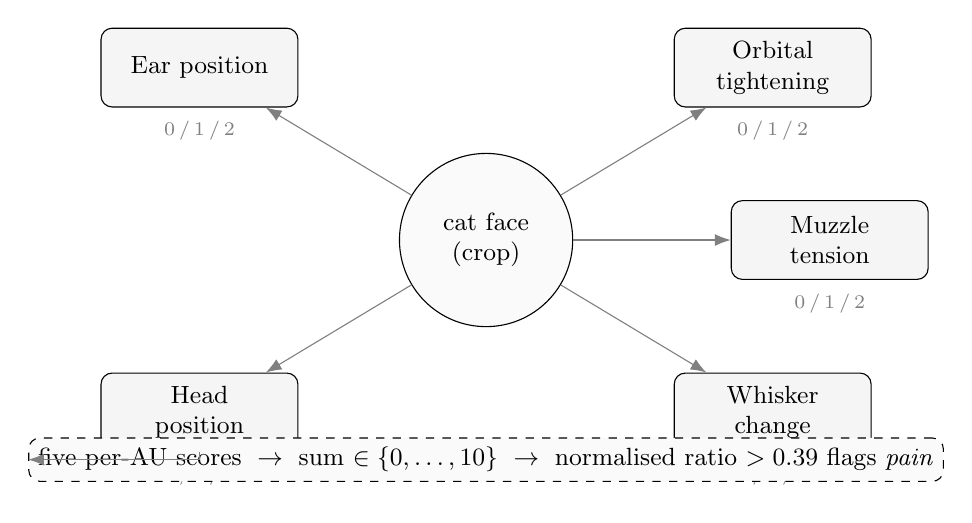
\begin{tikzpicture}[
      font=\small,
      au/.style={draw, rounded corners, minimum width=2.5cm, minimum height=1.0cm,
                 align=center, fill=gray!8},
      lvl/.style={font=\scriptsize\itshape, gray},
      every node/.style={align=center},
    ]
    % central face placeholder
    \node[draw, circle, minimum size=2.2cm, fill=gray!4] (face) {cat face\\(crop)};
    % five AUs around the face
    \node[au, above left=0.9cm and 1.6cm of face]  (ear)      {Ear position};
    \node[au, above right=0.9cm and 1.6cm of face] (orbital)  {Orbital\\tightening};
    \node[au, right=2.0cm of face]                 (muzzle)   {Muzzle\\tension};
    \node[au, below right=0.9cm and 1.6cm of face] (whisker)  {Whisker\\change};
    \node[au, below left=0.9cm and 1.6cm of face]  (head)     {Head\\position};
    % connectors
    \foreach \n in {ear,orbital,muzzle,whisker,head}{
      \draw[-{Latex[length=2mm]}, gray] (face) -- (\n);
    }
    % per-AU ordinal scale annotation
    \node[lvl, below=0.05cm of ear]     {$0\,/\,1\,/\,2$};
    \node[lvl, below=0.05cm of orbital] {$0\,/\,1\,/\,2$};
    \node[lvl, below=0.05cm of muzzle]  {$0\,/\,1\,/\,2$};
    \node[lvl, below=0.05cm of whisker] {$0\,/\,1\,/\,2$};
    \node[lvl, below=0.05cm of head]    {$0\,/\,1\,/\,2$};
    % aggregation note
    \node[draw, dashed, rounded corners, below=1.4cm of face, fill=gray!4,
          minimum width=8.2cm, align=center] (sum)
      {five per-AU scores $\;\rightarrow\;$ sum $\in\{0,\dots,10\}$
       $\;\rightarrow\;$ normalised ratio $>0.39$ flags \emph{pain}};
    \draw[-{Latex[length=2mm]}, gray] (head) |- (sum);
  \end{tikzpicture}
  \caption[The five FGS action units]{Schematic of the Feline Grimace Scale
    \autocite{evangelista2019}. Each of the five action units is scored on a
    three-level ordinal scale ($0/1/2$); the five scores are summed to a $0$--$10$
    composite and converted to a normalised ratio, with $>0.39$ flagging pain.
    This diagram fixes the target ontology used throughout the thesis; it is a
    structural schematic, not an example annotation. (Placeholder figure.)}
  \label{fig:fgs-five-au}
\end{figure}

A recent wave of machine-learning work has sought to automate this pipeline.
Two methodological families dominate. The first is \emph{landmark-then-geometry}:
a facial-landmark detector locates anatomical points, hand-engineered geometric
features are derived, and a classifier (frequently a gradient-boosted tree)
predicts pain or grimace score. Representative of this family,
\textcite{steagall2023} report an automated FGS pipeline reaching $95.5\%$
agreement using a minimum-aggregation rule over the whisker and head action units,
and \textcite{feighelstein2023} report a binary cat-pain classifier in which a
landmark-based model ($\approx 77\%$) outperformed a direct deep-learning
classifier ($\approx 65\%$), alongside an explainability analysis ranking the
mouth region above the eyes and ears in feature importance. The second family
relies on facial-landmark corpora to standardise the geometry: CatFLW provides
$48$ CatFACS-aligned landmarks per face with reported normalised mean error in
the $9$--$26\%$ range at roughly seven landmark-points of cost
\autocite{martvel2024catflw}. In parallel, foundation vision encoders such as
DINOv2 \autocite{oquab2023dinov2} have made it cheap to extract strong,
general-purpose facial features without task-specific pre-training, lowering the
data and compute floor for small-corpus ordinal modelling. Most recently, a COSMIN
scoping review of feline pain instruments has begun to systematise the
measurement-quality evidence for \emph{human-rater} instruments
\autocite{leesteagall2026}; automated scoring falls outside that review's topic
scope, so the question of what \emph{measurement} guarantees an automated scorer
should carry remains open.

\section{The gap, in our terms}
\label{sec:intro-gap}

The automated-FGS and binary-cat-pain literature, summarised above, is impressive
on its own terms---but those terms are accuracy on a single-source corpus. We
identify three gaps that this prior work does not address, and which together
motivate the present thesis.

\paragraph{(G1) No transportable trustworthiness method.}
Prior automated work optimises a point accuracy (or AUC) on one corpus and reports
it. What it does not produce is a \emph{method}---a piece of released, runnable
machinery that a future investigator can carry to the next corpus and re-run to
obtain a trustworthiness measurement. The headline number in
\textcite{steagall2023} or \textcite{feighelstein2023} is a fact about
\emph{their} dataset; it is not an instrument that travels. Because no open,
graded cat-FGS dataset exists, a contribution that is merely ``high accuracy on
corpus $X$'' is, for a feline-pain scorer, dead on arrival under independent
replication: a reviewer can dismiss it as a backbone swap on inaccessible data.
The portable artefact---the reusable measurement protocol---is the missing
deliverable.

\paragraph{(G2) No audit of capture-condition confounds.}
A facial-pain corpus is acquired under conditions (lighting, camera, restraint,
clinical context) that may correlate with the pain label itself. If brightness,
blur, aspect ratio, or background can predict the pain label, then a classifier
can score well by reading acquisition context rather than facial expression, and
the reported accuracy is an artefact of capture rather than evidence of pain
detection. Prior work does not systematically audit this entanglement, and---more
importantly---does not ship the audit as a protocol that the next corpus can run.

\paragraph{(G3) Low-prevalence measurement-error propagation is ignored.}
Acute clinical pain is a low-prevalence event in many realistic deployment
settings. At low prevalence, even small per-sample labelling and classification
errors propagate non-linearly into the operating characteristics that a clinician
actually relies upon. \textcite{chavoshi2025} make this concrete: at a $10\%$
prevalence, an instrument whose raw error looks benign can collapse to roughly
$53\%$ effective sensitivity once measurement error is propagated through the base
rate. A scorer reported only as a single accuracy figure, with no confidence
interval and no prevalence-aware operating point, silently hides this failure
mode.

These three gaps share a common root: the field reports \emph{performance} but not
\emph{trustworthiness}, and it reports both as corpus-bound numbers rather than
transportable methods. The present thesis is organised around closing that gap
without pretending to data we do not have.

\section{Objectives}
\label{sec:intro-objectives}

The thesis pursues four numbered objectives, ordered from the headline
\emph{portable method} down to the conceded engineering substrate.

\begin{enumerate}
  \item \textbf{Build a portable, power-aware confound-attribution protocol.}
    Construct a reusable, one-directional capture-condition audit (the
    FGS--BG--Gap, the per-AU energy-based pointing-game read as
    saliency-as-confound-evidence, EBPG, and a VLM judge-bias probe) that any
    future facial-pain-scorer corpus can run, at a pre-registered power, to
    detect---never to ``rule out''---entanglement between the pain label and
    acquisition context. Reporting is one-directional at this
    power~\autocite{adebayo2022posthoc}: the only honest conclusion is ``no
    confound detected at this power.'' This is the headline contribution, and it
    is validated today on planted positive and negative controls.
  \item \textbf{Provide a guarded VLM-as-AU-rater reliability check.} As a
    subordinate, inspected-not-validated reliability check, determine whether
    a frozen vision--language model (VLM) can weak-label the five FGS action units
    at \emph{human-rater agreement}---a $\kappa$ that measures weak-labelling
    capability only when the vet anchor is independent and the rubric handed to
    the VLM differs from the rubric the vet scored from, and otherwise measures
    rubric-following, so each run must state which it measures---quantified as a per-AU quadratic-weighted
    Cohen's $\kappa$ against a veterinary anchor, reported with a confidence-interval
    lower bound. The CI-lower-bound gate is textbook clinimetrics and the
    rubric-paraphrase guard is published practice; neither is claimed as novel.
    This check is retained as kill-tree insurance---the sole-survivor headline
    should the confound leg degrade---not as a co-equal second pillar.
  \item \textbf{Ship a welfare-asymmetric binary-plus-abstention decision floor.}
    Deliver a calibrated binary pain decision at a \emph{fixed} high-sensitivity
    operating point (pain-recall $\geq 0.90$, anchored to
    \textcite{evangelista2019}; never a symmetric Youden-$J$/$F_1$ knee), made
    visible through a welfare-asymmetric decision curve, with a defer-to-vet
    abstention boundary reported as a one-sided $95\%$ negative-predictive-value
    lower bound.
  \item \textbf{Build---but only inspect, not validate---a $0$--$10$ ordinal
    engine.} Implement a frozen DINOv2 encoder feeding five per-AU ordinal heads
    and a distributional decode to a $0$--$10$ composite, and ship it as an
    \emph{inspected-not-validated} exploratory layer. This engine is conceded as
    plumbing; it is never advanced as a validated graded claim.
\end{enumerate}

Objective~1 is the headline transportable contribution; Objective~2 is the
guarded reliability check that rides below it and serves as kill-tree insurance;
Objective~3 is the cited trustworthiness wrapper, an honest decision floor that
stands on its own even if the graded layer is dropped, but is supporting
evidence rather than a headline contribution; Objective~4 is built for
completeness and future extension but is firewalled out of every validated
results table. The contribution map is summarised in
Figure~\ref{fig:contribution-map}.

% ---------------------------------------------------------------------------
% Figure 1.2 — Thesis contribution map (TikZ).
% ---------------------------------------------------------------------------
\begin{figure}[t]
  \centering
  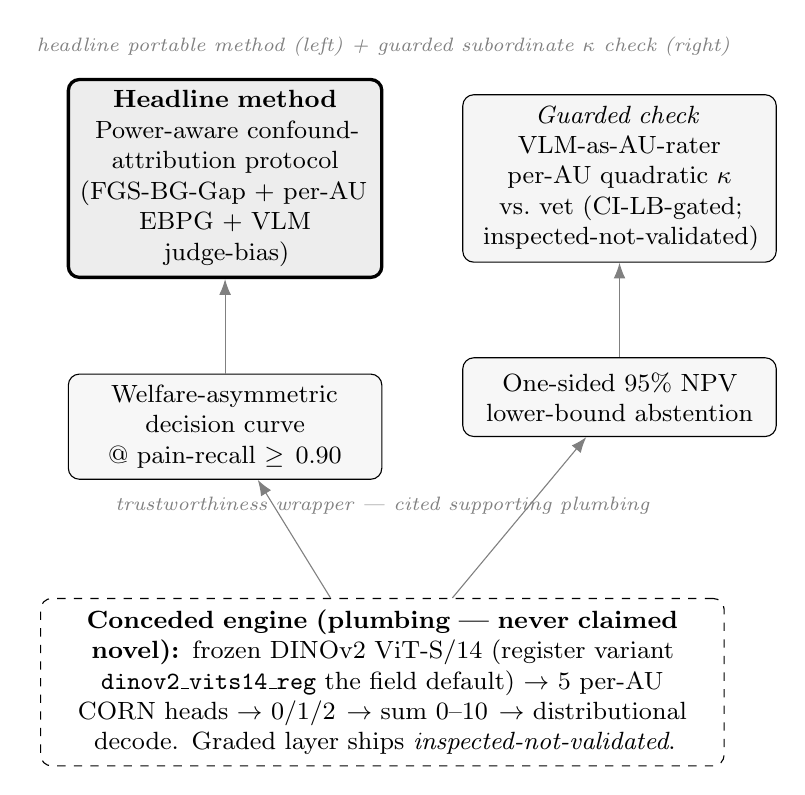
\begin{tikzpicture}[
      font=\small,
      box/.style={draw, rounded corners, minimum height=1.0cm, align=center,
                  text width=3.7cm, inner sep=4pt},
      head/.style={box, fill=gray!14, very thick},
      guard/.style={box, fill=gray!8},
      frame/.style={box, fill=gray!6},
      engine/.style={box, dashed, fill=white},
      lbl/.style={font=\scriptsize\itshape, gray},
    ]
    % headline portable method (left) + guarded subordinate check (right)
    \node[head] (m1) {\textbf{Headline method}\\Power-aware confound-\\attribution protocol\\(FGS-BG-Gap + per-AU\\EBPG + VLM judge-bias)};
    \node[guard, right=1.0cm of m1] (m2) {\emph{Guarded check}\\VLM-as-AU-rater\\per-AU quadratic $\kappa$\\vs.\ vet (CI-LB-gated;\\inspected-not-validated)};
    \node[lbl, above=0.15cm of m1.north east] {headline portable method (left) + guarded subordinate $\kappa$ check (right)};
    % the wrapper frame underneath
    \node[frame, below=1.2cm of m1, text width=3.7cm] (op)
      {Welfare-asymmetric decision curve\\@ pain-recall $\geq 0.90$};
    \node[frame, below=1.2cm of m2, text width=3.7cm] (ab)
      {One-sided $95\%$ NPV\\lower-bound abstention};
    \node[lbl, below=0.1cm of op.south east] {trustworthiness wrapper --- cited supporting plumbing};
    % conceded engine at the base, centred under the two wrapper frames
    \node[engine, below=1.5cm of op.south east, anchor=north, text width=8.4cm] (eng)
      {\textbf{Conceded engine (plumbing --- never claimed novel):}
       frozen DINOv2 ViT-S/14 (register variant \texttt{dinov2\_vits14\_reg} the
       field default) $\rightarrow$ 5 per-AU CORN heads $\rightarrow$
       $0/1/2 \rightarrow$ sum $0$--$10 \rightarrow$ distributional decode.
       Graded layer ships \emph{inspected-not-validated}.};
    % connectors
    \draw[-{Latex[length=2mm]}, gray] (eng) -- (op);
    \draw[-{Latex[length=2mm]}, gray] (eng) -- (ab);
    \draw[-{Latex[length=2mm]}, gray] (op) -- (m1);
    \draw[-{Latex[length=2mm]}, gray] (ab) -- (m2);
  \end{tikzpicture}
  \caption[Thesis contribution map]{Contribution map. The single headline
    deliverable is a portable, power-aware capture-condition
    confound-attribution protocol (top left). The VLM-as-AU-rater per-AU
    $\kappa$ protocol (top right) is a guarded, inspected-not-validated
    reliability check that rides below it as kill-tree insurance, not a co-equal
    second pillar. The trustworthiness wrapper (middle) supplies the
    welfare-asymmetric operating point and the abstention floor and is cited
    supporting plumbing rather than a headline. The DINOv2$+$CORN engine
    (bottom) is conceded plumbing and is never claimed as a contribution; its
    graded output ships inspected-not-validated. (Placeholder schematic.)}
  \label{fig:contribution-map}
\end{figure}

\section{Scope and honesty boundary}
\label{sec:intro-scope}

This thesis is, at the time of writing, a \emph{research proposal and methodology}
backed by a build specification; it reports an evaluation protocol, gate-conditioned
expected outcomes, and decision rules, rather than completed experimental results.
No accuracy, $\kappa$, or calibration number reported as ``ours'' appears in this
document, because no such experiment has yet been run. Literature numbers
(e.g.\ those of \textcite{evangelista2019}, \textcite{steagall2023},
\textcite{feighelstein2023}, \textcite{martvel2024catflw}, and
\textcite{chavoshi2025}) are reproduced only as background and are explicitly
attributed to their sources.

Several scope boundaries follow from honesty about what the project can and cannot
deliver, and are held as hard constraints throughout:

\begin{itemize}
  \item \textbf{Single corpus, single anchor.} The empirical substrate is a single
    forked Roboflow cat-pain corpus (binary pain / no\_pain boxes,
    $\sim 2040$ records / $\sim 1547$ distinct images, $\sim 12$--$13\%$
    prevalence, with a leaky shipped split that is discarded) plus one veterinary
    anchor whose size is fixed by an up-front power calculation. No open, graded
    cat-FGS dataset exists; CatFLW \autocite{martvel2024catflw} is used for
    eye-alignment landmarks only, not as a graded anchor, and an open
    horse-grimace set is used solely as a decode unit-test fixture (no horse
    number ever appears in a results table).
  \item \textbf{Solo compute.} The work is built by a single developer on an Apple
    M4 / MPS machine (no local CUDA); detector training alone is offloaded to a
    cloud T4, and the frozen encoder plus the ordinal heads run locally on cached
    features.
  \item \textbf{Decision-support framing only.} The output is a triage
    recommendation---``grimace consistent with pain, $X/10$; recommend veterinary
    assessment''---and \emph{never} an autonomous analgesia trigger. The negative
    class is documented as an unknown mixture (possibly sedated or post-operative
    animals), not as a clean ``no-pain'' reference.
  \item \textbf{Engine conceded.} The DINOv2$+$CORN engine is treated as plumbing
    throughout and is never claimed as a novel contribution; the word
    ``graded'' is struck from every validated-claim sentence, and the thesis
    abstract holds with the graded output dropped.
  \item \textbf{Anti-benchmark discipline.} The thesis never claims to ``beat''
    the $77\%$ / $79\%$ / $95\%$ figures of prior work. Every reported rate is
    accompanied by its distinct-pain-cat denominator and a Clopper--Pearson or
    bootstrap confidence interval, and accuracy is treated as an anti-benchmark
    rather than the objective.
\end{itemize}

\section{Research procedure}
\label{sec:intro-procedure}

The work is executed as a strict, blocking \emph{gate order}: each gate writes an
auditable artefact and blocks all downstream quantitative work until it passes.
The order is risk-first---the cheapest checks that can kill or reframe the project
run before any veterinary hour or GPU spend. The eight gates are summarised below
and depicted in Figure~\ref{fig:gate-flow}.

\begin{enumerate}
  \item \textbf{G0 --- Power calculations and vet-budget pre-registration.}
    Fix the single integer (how many faces the vet scores) by three zero-data
    power calculations: the faces needed for a per-AU $\kappa$ half-width
    $\leq 0.15$; the faces needed to certify a useful negative-predictive-value
    band at an acceptable abstention rate; and whether the $>0.39$ operating-point
    interval is reportable at the budgeted $n$. Blocks everything quantitative.
  \item \textbf{G1 --- Per-cat merge.} Collapse clips to true individuals,
    validated against trusted camera ids, so that no individual straddles a fold
    and the honest distinct-pain-cat denominator can be printed.
  \item \textbf{G2 --- Capture-condition confound audit.} Run the one-directional
    portable audit (Objective~2) before any spend; it can kill or reframe the
    corpus, and it publishes either way.
  \item \textbf{G3 --- Frozen, hashed, cat-disjoint hold-out.} Freeze and hash the
    test manifest so that a continuous-integration check aborts any run that can
    read it---structurally defeating post-hoc goalpost moves.
  \item \textbf{G4 --- MPS compute-correctness pre-checks (blocking).} Assert
    MPS-versus-CPU encoder logit parity and pass a synthetic ordinal
    decode-to-sum-to-threshold unit test, so that no number from silently-wrong
    hardware logits is ever believed.
  \item \textbf{G5 --- Alignment / normalised-mean-error gate.} Check that the
    detector crop is geometrically clean enough to feed the ordinal heads, adding
    a two-point eye-similarity alignment if not, so that ``calibration'' never
    silently measures crop quality.
  \item \textbf{G1-B --- Weak-label reliability $\kappa$ pilot.} Score the per-AU
    VLM-versus-vet quadratic $\kappa$ on the anchor (Objective~1); the pilot itself
    selects the VLM, and the gate fires on the $\kappa$ confidence-interval
    \emph{lower bound}, not the point estimate.
  \item \textbf{G6 --- Severity-cell count gate.} If the anchor yields only
    single-digit AU$=2$ (severe) cells, collapse the high end of the scale by a
    pre-committed rule rather than printing an uninformative per-cell number.
\end{enumerate}

% ---------------------------------------------------------------------------
% Figure 1.3 — Gate flow (TikZ).
% ---------------------------------------------------------------------------
\begin{figure}[t]
  \centering
  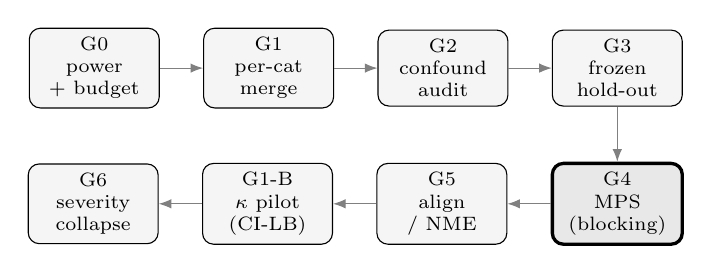
\begin{tikzpicture}[
      font=\scriptsize,
      gate/.style={draw, rounded corners, minimum width=1.65cm, minimum height=0.85cm,
                   align=center, fill=gray!8},
      block/.style={gate, fill=gray!18, very thick},
      flow/.style={-{Latex[length=1.6mm]}, gray},
    ]
    \node[gate] (g0) {G0\\power\\+ budget};
    \node[gate, right=0.55cm of g0] (g1) {G1\\per-cat\\merge};
    \node[gate, right=0.55cm of g1] (g2) {G2\\confound\\audit};
    \node[gate, right=0.55cm of g2] (g3) {G3\\frozen\\hold-out};
    \node[block, below=0.7cm of g3] (g4) {G4\\MPS\\(blocking)};
    \node[gate, left=0.55cm of g4] (g5) {G5\\align\\/ NME};
    \node[gate, left=0.55cm of g5] (g1b) {G1-B\\$\kappa$ pilot\\(CI-LB)};
    \node[gate, left=0.55cm of g1b] (g6) {G6\\severity\\collapse};
    \draw[flow] (g0) -- (g1);
    \draw[flow] (g1) -- (g2);
    \draw[flow] (g2) -- (g3);
    \draw[flow] (g3) -- (g4);
    \draw[flow] (g4) -- (g5);
    \draw[flow] (g5) -- (g1b);
    \draw[flow] (g1b) -- (g6);
  \end{tikzpicture}
  \caption[Gate run-order]{The blocking gate run-order
    (G0 $\rightarrow$ G1 $\rightarrow$ G2 $\rightarrow$ G3 $\rightarrow$ G4
    $\rightarrow$ G5 $\rightarrow$ G1-B $\rightarrow$ G6). Each gate emits an
    auditable artefact and blocks downstream quantitative work; G4 (MPS
    compute-correctness) is hard-blocking. The order is risk-first: the cheapest
    kill-or-reframe checks run before any veterinary or GPU spend.}
  \label{fig:gate-flow}
\end{figure}

A kill/pivot rule is attached to the gate order: if the orbital, ear, or head
$\kappa$ lower bound at G1-B falls below its pre-registered floor, the graded
layer is dropped entirely and the project ships the calibrated
binary-plus-abstention floor with the confound protocol; the headline confound
protocol still stands, because it is validated independently of the $\kappa$
result. Conversely, the $\kappa$ check is retained as kill-tree insurance: should
the confound leg itself degrade, the $\kappa$ check---once the independent per-AU
vet anchor exists---becomes the sole-survivor headline, because it measures a
real fact whether the result is strong or mediocre.

\section{Expected benefits and contributions}
\label{sec:intro-contributions}

The thesis is designed so that its value does not depend on any single experiment
firing favourably. Its expected contributions are one headline released,
dataset-agnostic method, a guarded reliability check below it, and a cited
supporting wrapper:

\begin{enumerate}
  \item \textbf{A portable, power-aware capture-condition confound-attribution
    protocol (the headline).} The one-directional FGS--BG--Gap plus per-AU
    EBPG-as-confound-evidence audit, augmented by a VLM judge-bias probe and run
    at a pre-registered power, runnable on any future facial-pain-scorer corpus,
    whose deliverable is the protocol itself rather than a verdict about one
    dataset. It is validated today on planted positive and negative controls and
    reports one-directionally at this power~\autocite{adebayo2022posthoc}. The
    claimed novelty is the assembly, the per-AU
    EBPG-as-confound-evidence reading, and the instantiation of
    equivalence-style audit hygiene---never any individual primitive or the
    underlying statistics.
  \item \textbf{A guarded VLM-as-AU-rater $\kappa$ reliability check (subordinate;
    result pending the independent vet anchor).} Released code that
    scores any face corpus's per-AU VLM labels against a veterinary anchor and
    reports five quadratic-weighted $\kappa$ values with confidence-interval lower
    bounds. The forked corpus's numbers merely \emph{instantiate} the check;
    the deliverable is the reusable machinery; the number it will
    eventually produce---whether a frozen VLM weak-labels feline FGS action
    units at human-rater agreement---remains pending the independent per-AU
    vet anchor (Gate 0), since the current binary corpus cannot yield $0/1/2$
    AU ground truth. The CI-lower-bound gate is textbook clinimetrics and the
    rubric-paraphrase guard is published; neither is a novel increment. This check
    is kill-tree insurance, not a co-equal headline.
  \item \textbf{A welfare-asymmetric decision-curve and abstention floor (cited
    supporting plumbing).} An
    operating point fixed at high sensitivity with the undertreat-to-overtreat
    harm ratio swept as a range, plus a defer-to-vet boundary reported with
    finite-sample one-sided lower bounds. This is the clinical-decision
    component that distinguishes the trustworthiness wrapper from generic
    calibration, and it makes the low-prevalence error-propagation concern of
    \textcite{chavoshi2025} an explicit, reported quantity rather than a hidden
    failure mode. It is supporting evidence, not a headline contribution.
\end{enumerate}

Taken together these artefacts answer the three gaps of
Section~\ref{sec:intro-gap} without overclaiming: they supply the transportable
trustworthiness method (G1), the capture-condition audit (G2), and the
prevalence-aware operating point (G3) that the prior automated-FGS literature
leaves open. The remainder of the thesis develops each in turn---the FGS and
automated-scoring background and the measurement-quality literature
(Chapter~2), the methodology and gate-bound evaluation protocol, and the
gate-conditioned expected outcomes and decision rules---always under the standing
constraint that the DINOv2$+$CORN engine is conceded plumbing and that no graded
claim is ever validated.

%====================================================================
% Chapter 2 — Background and Related Work
% Self-contained section file: no preamble, no \documentclass.
% Requires (provided by main.tex preamble): booktabs, tikz, amsmath,
% biblatex/natbib. TikZ libraries used: positioning, arrows.meta, fit.
%====================================================================
\chapter{Background and Related Work}
\label{ch:background}

This chapter follows the two-part recipe of a conventional literature review: a
concise technical primer that fixes the vocabulary used throughout the rest of
this document (Section~\ref{sec:bg-primer}), and a per-paper survey of the
feline and animal facial-pain literature that situates our work
(Section~\ref{sec:bg-related}). It closes with a synthesis
(Section~\ref{sec:bg-synthesis}) that contrasts prior work against the two
\emph{portable methods} this project headlines, and makes the
\enquote{not-a-replicate} argument explicit by enumerating the replication
traps a single-corpus cat-pain study must avoid.

A framing rule governs the whole chapter and is stated once here so it need not
be repeated: the modelling \emph{engine} of this project---a frozen DINOv2
backbone feeding rank-consistent ordinal heads---is treated as conceded
\emph{plumbing} and is never claimed as a novel contribution. The primer
therefore describes these components only to the depth needed to read the
method, not as from-scratch tutorials, and the synthesis is careful to locate
novelty exclusively in the two measurement protocols, not in the architecture.

\section{Technical background}
\label{sec:bg-primer}

\subsection{The Feline Grimace Scale and its action-unit rubric}
\label{subsec:bg-fgs}

The Feline Grimace Scale (FGS) is an observational pain instrument that scores a
cat's facial expression along five \emph{action units} (AUs): ear position,
orbital tightening, muzzle tension, whisker change, and head position. Each AU
is scored on a three-point ordinal scale ($0$~=~action unit absent,
$1$~=~moderately present or uncertain, $2$~=~obviously present), and the five
scores are summed and rescaled to a $0$--$10$ index; a normalised ratio
$\geq 0.39$ is the published decision boundary indicating that analgesia should
be considered \cite{evangelista2019}. The rubric wording adopted by the VLM
weak-labeller in this project is taken verbatim from this scale, so that the
labelling target is the same construct the validation study certified rather
than a paraphrase. Figure~\ref{fig:fgs-schematic} shows the AU-to-score
schematic that the rest of this document refers to.

Two properties of the scale matter for the methods that follow. First, the AU
scores are \emph{ordinal, not nominal}: a confusion of $0$ with $2$ is a larger
error than a confusion of $0$ with $1$, which is why every agreement and
calibration metric in this work is ordinal-aware rather than treating the three
levels as unordered classes. Second, the summed index is a
\emph{convolution of five low-cardinality variables}; the resulting $0$--$10$
sum has only eleven atoms, a fact that later forbids drawing a binned
reliability diagram over the sum (Section~\ref{subsec:bg-calibration}).

\begin{figure}[t]
  \centering
  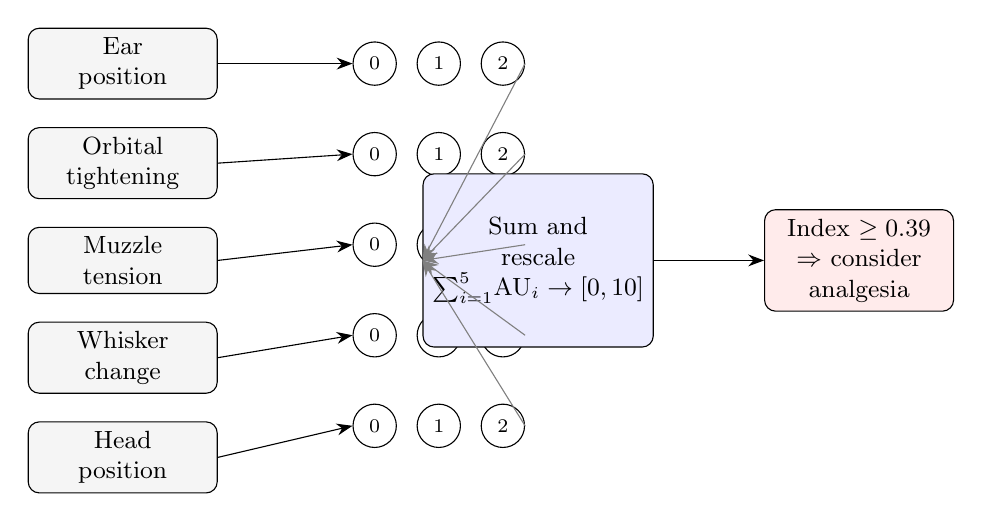
\begin{tikzpicture}[
      font=\small,
      au/.style={draw, rounded corners, minimum width=2.4cm,
                 minimum height=0.8cm, align=center, fill=gray!8},
      lvl/.style={draw, circle, minimum size=0.55cm, inner sep=0pt,
                  font=\scriptsize},
      node distance=0.35cm and 1.4cm,
      >={Stealth[length=2mm]}
    ]
    % five AUs
    \node[au] (ear)  {Ear\\position};
    \node[au, below=of ear]    (orb) {Orbital\\tightening};
    \node[au, below=of orb]    (muz) {Muzzle\\tension};
    \node[au, below=of muz]    (whk) {Whisker\\change};
    \node[au, below=of whk]    (hed) {Head\\position};

    % per-AU ordinal levels
    \foreach \n/\y in {ear/0, orb/-1.15, muz/-2.3, whk/-3.45, hed/-4.6} {
      \node[lvl] (\n0) at (3.2,\y) {0};
      \node[lvl, right=0.25cm of \n0] (\n1) {1};
      \node[lvl, right=0.25cm of \n1] (\n2) {2};
      \draw[->] (\n.east) -- (\n0.west);
    }

    % aggregation node
    \node[au, fill=blue!8, minimum height=2.2cm, right=2.6cm of muz]
      (sum) {Sum and\\rescale\\$\sum_{i=1}^{5}\!\mathrm{AU}_i \to [0,10]$};
    \foreach \n in {ear,orb,muz,whk,hed} {
      \draw[->, gray] (\n2.east) -- (sum.west);
    }

    % decision
    \node[au, fill=red!8, right=1.4cm of sum] (dec)
      {Index $\geq 0.39$\\$\Rightarrow$ consider\\analgesia};
    \draw[->] (sum.east) -- (dec.west);
  \end{tikzpicture}
  \caption[FGS action-unit to score schematic]{The Feline Grimace Scale maps
    five facial action units, each scored ordinally on $\{0,1,2\}$, to a summed
    $0$--$10$ index, with a published decision threshold at the normalised ratio
    $0.39$ \cite{evangelista2019}. In this project the per-AU rubric is the
    weak-labelling target; summation and the $0.39$ flag are computed in code,
    never elicited from the rater.}
  \label{fig:fgs-schematic}
\end{figure}

\subsection{Ordinal regression and rank consistency}
\label{subsec:bg-ordinal}

Because each AU is an ordered three-level variable, predicting it with a plain
softmax classifier discards the ordering and admits rank-inconsistent
probability estimates (e.g.\ assigning high mass to $\Pr(\mathrm{AU}\geq 2)$
while assigning low mass to $\Pr(\mathrm{AU}\geq 1)$). The CORAL framework
\cite{cao2020coral} reformulates a $K$-level ordinal problem as $K-1$ binary
\enquote{is the label greater than rank $k$?} sub-tasks that share a single
feature projection plus per-rank biases, which guarantees the predicted
cumulative probabilities are monotone and hence rank-consistent. CORN
\cite{shi2023corn} relaxes the weight-sharing constraint of CORAL by conditioning
each rank's probability on the previous one through the chain rule, recovering
rank consistency without sacrificing the flexibility of independent rank
classifiers; it is the head we adopt for each AU. The relevant output is the set
of soft cumulative probabilities $\Pr(\mathrm{rank} > k)$, from which a per-AU
probability mass function over $\{0,1,2\}$ is read off. A captioned placeholder
for this head is shown in Figure~\ref{fig:corn-placeholder}; the convolution of
the five per-AU PMFs into a distribution over the $0$--$10$ sum is the
\emph{distributional decode} used for the calibration metrics below.

\begin{figure}[t]
  \centering
  \fbox{\parbox{0.86\linewidth}{\centering\vspace{0.4cm}
    \textbf{[Schematic placeholder --- to be produced]}\\[0.3cm]
    \small CORN rank-consistent ordinal head: a frozen feature vector feeds a
    shallow projection producing $K-1=2$ conditional rank logits per action
    unit; $\Pr(\mathrm{rank}>0)$ and $\Pr(\mathrm{rank}>1)$ are chained into a
    monotone cumulative profile and decoded to a PMF over $\{0,1,2\}$. Five such
    heads are convolved into a PMF over the $0$--$10$ sum.\vspace{0.4cm}}}
  \caption[CORN ordinal head schematic (placeholder)]{Captioned placeholder for
    the per-AU CORN head \cite{shi2023corn,cao2020coral}. No results are
    depicted; this is a structural diagram to be rendered in the methods
    chapter.}
  \label{fig:corn-placeholder}
\end{figure}

\subsection{Self-supervised frozen vision features}
\label{subsec:bg-dinov2}

DINOv2 \cite{oquab2023dinov2} is a self-supervised vision transformer trained
without labels on a large curated image corpus, producing general-purpose
features that transfer to downstream tasks without fine-tuning. We use a frozen
DINOv2 ViT-S/14 encoder purely as a fixed feature extractor: the backbone is
never updated, its pooled features are cached to disk once, and only the shallow
CORN heads are trained on the cache. This is the appropriate low-data choice on
the available hardware---fully fine-tuning a transformer on a few hundred faces
would overfit catastrophically---and it is deliberately unremarkable. The
backbone is part of the conceded engine; we make no claim that the choice of
self-supervised features is itself a contribution.

\subsection{Vision--language models as structured raters}
\label{subsec:bg-vlm}

A vision--language model (VLM) can be prompted to read an image and emit a
structured answer. We use this capability narrowly: the VLM is constrained by a
forced tool-use schema to return five ordinal AU scores, each a closed
enumeration over $\{0,1,2\}$, with a rationale produced before each score. The
VLM is therefore a \emph{weak labeller} that proposes per-AU FGS scores at
scale and cheaply, which a veterinarian then accepts or corrects. The central
empirical question this raises---and the first headline of this work---is
whether such a frozen VLM can weak-label feline FGS action units at
human-rater agreement, measured against a veterinary anchor. That measurement,
not the act of prompting a VLM, is the contribution; the rater is selected by
its measured agreement rather than asserted to be adequate.

\subsection{Calibration and the expected calibration error}
\label{subsec:bg-calibration}

A model is \emph{calibrated} when its stated probabilities match empirical
frequencies. The expected calibration error (ECE) summarises miscalibration by
binning predictions and comparing confidence to accuracy within each bin;
temperature scaling \cite{guo2017calibration} is a one-parameter post-hoc fix
that rescales logits to reduce ECE without changing the ranking of predictions.
For the ordinal AUs we report a \emph{per-AU classwise} ECE so that
miscalibration is attributable to a specific action unit, and we calibrate each
CORN head with a single temperature scalar fit on training folds. A deliberate
restriction follows from Section~\ref{subsec:bg-fgs}: because the $0$--$10$ sum
has only eleven atoms, a binned reliability diagram on the sum is degenerate at
this sample size, so the distributional path reports a ranked probability score
on the sum plus per-AU classwise ECE, and \emph{no} binned reliability diagram
on the sum is ever drawn. Calibration is supporting hygiene in this work, not a
headline.

\subsection{Decision curve analysis and net benefit}
\label{subsec:bg-dca}

Generic accuracy and calibration metrics ignore that the two error types of a
welfare instrument are not equally costly: failing to flag a painful cat is far
worse than over-flagging a comfortable one. Decision curve analysis
\cite{vickers2006dca} addresses this by plotting \emph{net benefit} against a
threshold probability that encodes the clinician's relative weighting of the two
errors, allowing a model to be judged across a \emph{range} of harm ratios
rather than at a single symmetric-cost operating point. Because we have no
veterinarian-elicited undertreat:overtreat ratio, we sweep the ratio as a range
along the threshold-probability axis. This welfare-asymmetric decision curve is
the headline artifact of the trustworthiness wrapper---a clinical-decision
contribution that distinguishes the wrapper from generic calibration---and the
operating point itself is selected at a fixed pain-recall $\geq 0.90$ anchored
to the FGS validation study, never at a symmetric Youden-$J$ or $F_1$ knee.

\subsection{Conformal risk control: Learn-Then-Test}
\label{subsec:bg-ltt}

Learn-Then-Test (LTT) \cite{angelopoulos2021ltt} is a distribution-free,
finite-sample procedure for choosing model thresholds so that a user-specified
risk is controlled with high probability. We use it for the defer-to-vet
abstention rule: two thresholds bracket the $0.39$ point so that confident
negatives and confident positives are returned while the uncertain middle is
deferred, and LTT certifies a one-sided lower bound on the negative predictive
value (NPV, i.e.\ control of missed pain) at each abstention rate. The output is
reported strictly as a \emph{lower bound}; the word \enquote{guaranteed} is
banned, and if the available label budget cannot certify a useful band the
abstention curve is reported as exploratory rather than as a controlled claim.

\subsection{Inter-rater agreement: weighted kappa and Krippendorff's alpha}
\label{subsec:bg-agreement}

Agreement between two raters on an ordinal scale is measured with the
quadratically weighted kappa \cite{cohen1968kappa}, which penalises
disagreements by the squared distance between levels and is therefore the
correct statistic for the three-level AUs (a nominal kappa over
$\{0,1,2\}$ without weights is a bug to avoid). The headline measurement of this
project is exactly such a per-AU quadratic weighted kappa between the VLM and
the veterinary anchor, gated on its confidence-interval \emph{lower bound}
rather than the point estimate, because at the small anchor sizes available a
point estimate of $0.6$ is statistically indistinguishable from a true value of
$0.47$. Separately, Krippendorff's alpha \cite{krippendorff2004} in its ordinal
form measures the self-consistency of the VLM across repeated runs at non-zero
temperature; this is a vet-free reliability pre-screen and an abstention signal,
and it complements but never substitutes for the vs-vet kappa.

\subsection{Confident learning for label triage}
\label{subsec:bg-confident}

Confident learning \cite{cleanlab2021} estimates which labels in a noisy dataset
are likely wrong by analysing the joint distribution of given and predicted
labels. We use it not to clean labels automatically but to \emph{triage} the
scarce veterinary review budget: images that confident learning flags as likely
mislabelled, together with VLM disagreements and near-threshold cases, are sent
to the veterinarian first, maximising label corrections per review minute.

\subsection{Background robustness and saliency faithfulness}
\label{subsec:bg-robustness}

A face-pain classifier can appear accurate while reading the wrong signal---
lighting, background, or capture conditions correlated with the pain label
rather than the face itself. The backgrounds-challenge line of work
\cite{xiao2021background} demonstrates that models routinely exploit such
spurious foreground/background cues and provides the conceptual basis for our
\emph{capture-condition confound audit}: a trivial classifier built on
brightness, blur, aspect ratio, and generic embedding features is trained to
predict pain, and if it beats chance the label is entangled with acquisition
context. Complementarily, the energy-based pointing game from the Score-CAM line
\cite{wang2020scorecam} quantifies saliency \emph{faithfulness}---how much of a
saliency map's energy falls inside the relevant region---and underlies the
per-AU energy-based pointing game (EBPG) we report alongside the
foreground/background gap (FGS-BG-Gap). Crucially this audit is
\emph{one-directional}: it is well powered to \emph{detect} confounding but
underpowered to rule it out, so its only honest conclusion is \enquote{no
confound detected at this power,} never \enquote{no confound.} The
\emph{protocol}---FGS-BG-Gap plus per-AU EBPG, runnable on any future
facial-pain corpus---is the second headline contribution, distinct from any
verdict about a particular dataset.

\section{Related feline and animal pain work}
\label{sec:bg-related}

Each entry below follows the same recipe: aim, method, the key reliability
statistic the authors report, and the limitation that bears on our design. The
reported numbers belong to the cited studies and are quoted here as background;
this project has not yet run experiments and reports no results of its own.

\subsection{FGS validation (Evangelista et al.)}
The aim was to construct and validate the Feline Grimace Scale as an
observational acute-pain instrument \cite{evangelista2019}. The method paired
human raters scoring the five AUs against established pain references, with
psychometric validation of reliability, criterion validity, and a decision
threshold. The headline reliability statistics are an area under the curve of
approximately $0.94$ with sensitivity around $90.7\%$ and specificity around
$86.6\%$ at the normalised-ratio threshold of $0.39$. The limitation for us is
that this is a \emph{human-rater} instrument: it certifies that trained people
scoring the rubric recover pain, not that any automated pipeline does, and it
fixes the construct and the operating anchor (pain-recall $\geq 0.90$) we
inherit rather than a model to compare against.

\subsection{Automated landmark FGS (Steagall et al.)}
The aim was to automate FGS scoring from images \cite{steagall2023}. The method
detected facial landmarks, derived geometric features from them, and classified
with a gradient-boosted model (XGBoost), with a minimum-aggregation rule across
whisker and head regions. The reported headline accuracy is about $95.5\%$. Two
limitations shape our positioning: the pipeline is a \emph{landmark-geometry}
approach that we deliberately do not replicate (it is one of the replication
traps in Section~\ref{sec:bg-synthesis}), and a single bare accuracy figure on
its own corpus is precisely the anti-benchmark we refuse to compete against on
headline terms.

\subsection{Explainable binary cat-pain detection (Feighelstein et al.)}
The aim was binary cat-pain detection with explanation \cite{feighelstein2023}.
The method compared a landmark-based classifier (reported around $77\%$) against
a deep-learning classifier (reported around $65\%$), with an explainability
analysis indicating the mouth region contributed more than the eyes, which
contributed more than the ears, and a two-source pain ground-truth rule
(a composite pain-scale threshold together with a charted clinical reason). The
limitation is that this is a \emph{binary} detector on a related corpus; without
the firewall and per-cat grouping we adopt, the natural next paper is a
backbone-swapped re-run of exactly this, which is the study we are explicitly
trying not to write.

\subsection{CatFLW landmarks (Martvel et al.)}
The aim was a cat facial-landmark dataset and detector \cite{martvel2024catflw}.
The method provided CatFACS-aligned facial landmarks with reported normalised
mean error in roughly the $9$--$26\%$ range at a modest landmark count. The
limitation, and the reason it is preprocessing rather than an anchor in our
pipeline, is that it carries landmarks and bounding boxes but \emph{no pain or
AU labels}; treating it as a graded FGS anchor would be a category error.
We use it only for an eye-alignment / NME audit to confirm crops are
geometrically clean enough to feed the ordinal heads.

\subsection{COSMIN scoping review of human-rater instruments (Lee \& Steagall)}
The aim was a COSMIN-style scoping review of the measurement properties of
feline pain instruments \cite{leesteagall2026}. The method screened and
appraised \emph{human-rater} pain-assessment instruments against measurement-
property criteria. The limitation that governs how we cite it is one of scope:
the review covers human-rater instruments only, and automated/AI scoring is
outside its topical remit. We therefore do not claim the review named
calibration or confidence intervals as gaps, nor that it excluded automated
scorers as a finding---it simply did not address them.

\subsection{Low-prevalence measurement-error propagation (Chavoshi et al.)}
The aim was to characterise how measurement error propagates at low disease
prevalence \cite{chavoshi2025}. The method analysed how imperfect labels and
classifiers degrade effective performance as prevalence falls, with a worked
illustration in which a nominally strong classifier collapses to roughly $53\%$
effective sensitivity around $10\%$ prevalence. The implication for us is direct
and sobering: our corpus sits near $12$--$13\%$ pain prevalence, so headline
accuracy is the wrong target, confidence intervals and a fixed-high-sensitivity
operating point are mandatory, and any single-number boast would be misleading
in exactly the regime this paper formalises.

\section{Synthesis and positioning}
\label{sec:bg-synthesis}

\subsection{What is new here, and what is conceded}
The prior work above clusters into two families: detectors that report a single
accuracy figure on their own corpus
\cite{steagall2023,feighelstein2023}, and the instrument/measurement context
that frames them \cite{evangelista2019,leesteagall2026,chavoshi2025} plus the
landmark scaffolding \cite{martvel2024catflw}. Our contribution is deliberately
\emph{not} a better detector. It is two transportable measurement protocols that
no prior feline-pain study produced: (i) a measurement of whether a frozen VLM
can weak-label FGS action units at human-rater agreement, expressed as five
per-AU quadratic weighted kappas against a veterinary anchor and gated on the
confidence-interval lower bound; and (ii) a reusable capture-condition
confound-attribution protocol (FGS-BG-Gap plus per-AU EBPG), one-directional by
construction. The DINOv2-plus-CORN engine carrying these methods is conceded as
plumbing and is never claimed as novel; the binary-plus-wrapper spine ships with
a welfare-asymmetric decision curve and a one-sided NPV lower-bound abstention
curve, while the $0$--$10$ ordinal layer ships inspected-but-not-validated.
Table~\ref{tab:positioning} contrasts the prior work with this positioning, with
accuracy treated explicitly as an anti-benchmark and a column marking whether a
contribution is a \emph{portable method}.

\begin{table}[t]
  \centering
  \caption[Prior work versus this work positioning matrix]{Positioning matrix.
    Accuracy figures are quoted from the cited studies as background and are
    treated as an \emph{anti-benchmark}: this work does not compete on a single
    corpus accuracy. The final column marks whether the contribution is a
    dataset-agnostic \emph{portable method}. Quoted statistics are the original
    authors'; this project reports no results.}
  \label{tab:positioning}
  \small
  \begin{tabular}{@{}p{3.0cm}p{3.1cm}p{3.3cm}cc@{}}
    \toprule
    \textbf{Work} & \textbf{Method} & \textbf{Reported reliability stat
      (theirs)} & \textbf{Task} & \textbf{Portable method?} \\
    \midrule
    Evangelista et al.\ \cite{evangelista2019}
      & Human-rater FGS, validated
      & AUC $\approx 0.94$; sens.\ $90.7\%$; spec.\ $86.6\%$ at $0.39$
      & Graded (human) & No (instrument) \\
    Steagall et al.\ \cite{steagall2023}
      & Landmark geometry $\to$ XGBoost
      & Acc.\ $\approx 95.5\%$
      & Graded (auto) & No \\
    Feighelstein et al.\ \cite{feighelstein2023}
      & Landmark vs.\ deep, with XAI
      & Acc.\ $\approx 77\%$ (landmark) / $65\%$ (DL)
      & Binary & No \\
    Martvel et al.\ \cite{martvel2024catflw}
      & CatFACS landmark detector
      & NME $\approx 9$--$26\%$
      & Landmarks & No (no pain labels) \\
    Lee \& Steagall \cite{leesteagall2026}
      & COSMIN scoping review
      & Measurement-property appraisal (human raters only)
      & Review & No \\
    Chavoshi et al.\ \cite{chavoshi2025}
      & Error-propagation analysis
      & $\sim 53\%$ eff.\ sens.\ at $10\%$ prevalence
      & Theory & Yes (transfers) \\
    \midrule
    \textbf{This work (i)}
      & VLM-as-AU-rater, vs.-vet kappa
      & \emph{CI-lower-bound-gated per-AU QWK (to be measured)}
      & AU rating & \textbf{Yes} \\
    \textbf{This work (ii)}
      & Confound-attribution protocol
      & \emph{FGS-BG-Gap + per-AU EBPG (one-directional)}
      & Audit & \textbf{Yes} \\
    \textbf{This work (frame)}
      & Welfare-asymmetric DCA + LB-abstention
      & \emph{net benefit (range); one-sided 95\% NPV LB}
      & Binary wrapper & \textbf{Yes} \\
    \bottomrule
  \end{tabular}
\end{table}

\subsection{The not-a-replicate case and eight replication traps}
\label{subsec:bg-traps}

Because this project is instantiated on a single in-domain corpus, the most
likely way it could collapse into \enquote{another cat-pain detector} is by
falling into one of a small set of replication traps. We name them here so the
methods chapter can be read as a list of deliberate avoidances:

\begin{enumerate}
  \item \textbf{Landmark-geometry replication.} Re-implementing the Steagall
    landmark-to-XGBoost pipeline \cite{steagall2023}; we use frozen features and
    ordinal heads precisely to not retread it.
  \item \textbf{Binary-detector replication.} Producing a backbone-swapped
    re-run of the Feighelstein binary detector \cite{feighelstein2023}; the
    portable methods, not the detector, are the headline.
  \item \textbf{Video/temporal replication.} Borrowing temporal landmark-track
    machinery; out of scope and not what the corpus supports.
  \item \textbf{External-cohort overclaim.} Asserting cross-cohort
    generalisation from a corpus dominated by a single known camera identity.
  \item \textbf{Single-rater ICC overclaim.} Reporting multi-rater agreement
    statistics when only one veterinary anchor exists.
  \item \textbf{Accuracy-as-benchmark.} Writing \enquote{we beat $77/79/95\%$};
    we always print the distinct-pain-cat denominator with Clopper--Pearson or
    bootstrap intervals, and never compete on a single corpus accuracy.
  \item \textbf{Cross-species headline.} Carrying a horse-grimace number into
    the abstract, results, or any transfer table; the horse set is decode
    scaffolding for a unit test only.
  \item \textbf{Validated-graded overclaim.} Reporting the $0$--$10$ graded
    layer as a validated instrument; it ships inspected-but-not-validated, and
    the word \enquote{graded} is struck from every validated-claim sentence.
\end{enumerate}

Avoiding these eight traps is what converts a single-corpus study into a
contribution that survives the obvious \enquote{swap the backbone and add
metrics} critique: the two surviving claims are facts about the world (a
measured VLM-vs-vet agreement) and a reusable audit protocol, both portable to
the next dataset, riding on an explicitly conceded engine.

% !TEX root = ../main.tex
% Chapter 3 --- Data and Materials
% Self-contained section file: no preamble, no \documentclass.
% Requires the document preamble to load: booktabs, tikz, biblatex/natbib.
% TikZ libraries assumed available: positioning, arrows.meta, shapes.geometric, fit, backgrounds, calc.

\chapter{Data and Materials}
\label{ch:data}

This chapter documents every data source the project touches, the role each
plays, and the data-hygiene facts that constrain what can honestly be claimed
from them. It deliberately mirrors the template's data-acquisition chapter
(collection flow, inclusion/exclusion, expert re-check) but adapts that
structure to a \emph{multi-source} reality in which a single in-domain binary
corpus is surrounded by scaffolding, preprocessing, and unit-test fixtures that
must never be allowed to co-mingle. Two framing rules govern the entire
chapter and are stated once here so that they need not be re-litigated at every
table. First, the only source of trustworthy graded (per-action-unit, $0/1/2$)
labels is a vet anchor that is \emph{produced}, not downloaded
(Section~\ref{sec:vet-anchor}); this anchor powers only the subordinate, guarded
reliability check and the cited welfare-wrapper plumbing, \emph{not} the
chapter's headline contribution, which is the confound-attribution protocol of
Chapter~\ref{ch:vlm-wrapper} and is validated on planted synthetic controls
without any vet labels. Second, this is a methodology document and we have run
no experiments, so the chapter reports the data \emph{contract} rather than
results. Crucially, the corpus has not yet been forked: the project's
\texttt{data/} substrate is empty at the time of writing, so every corpus count
below --- the $\approx 2040$ records, the $\approx 1547$ distinct images, the
$493$ duplicate filenames, the $\approx 12.7\%$ prevalence, the $336$ source
clips, and the $84$ \texttt{CAT\_01} clips --- is a \emph{projected pre-fork
target} read off the unforked Roboflow source, not a measured or audited
quantity. The figures fix the data contract and the planning targets; they are
never invented results, but neither are they yet measurements.

\section{The forked Roboflow cat-pain corpus --- the binary spine}
\label{sec:roboflow-spine}

\subsection{Purpose and provenance}

The single in-domain corpus is a public Roboflow detection project
(\texttt{lia-k4jkv/cat-pain-ul7lu}) that the project \emph{plans} to fork and
re-host in the workspace as
\texttt{mingraths-workspace/cat-pain-ul7lu-p3rtl}; that fork has not yet been
executed, so the description here is of the intended binary spine rather than an
in-hand corpus. Once forked it will be the only set that lives in the cat-pain
namespace, carrying the full weight of the binary spine: it is to train the
binary pain detector and supply the tight head crops that feed the frozen image
encoder. The unforked source is projected to comprise roughly $2040$ records
that resolve to approximately $1547$ distinct images after de-duplication
(Section~\ref{subsec:hygiene}); these are pre-fork targets, not measured counts. Its upstream provenance is the Zhang/Sun/Tang
2008 Flickr cat-head family of photographs; this is an important honesty point,
because the negative class is therefore a heterogeneous collection of generic
internet cat photographs rather than a clinically curated control group. The
corpus is released under CC~BY~4.0 according to its project metadata, which
makes a derived release possible \emph{provided} it is kept walled from the
non-commercial CatFLW images discussed in
Section~\ref{subsec:catflw} (the license-co-mingling firewall of
Section~\ref{sec:datasheet}).

\subsection{What labels it carries, and what it does not}

The corpus carries binary \texttt{pain}\,/\,\texttt{no\_pain} bounding boxes and
nothing else: there are \emph{zero} per-action-unit, $0$--$10$, or
Feline Grimace Scale (FGS) labels anywhere in it. This is the structural reason
the project cannot derive a graded FGS instrument from this corpus alone, and
it motivates the validated framework of the published FGS literature
\citep{evangelista2019} being used only as background rather than as a label
source. Equally load-bearing is the composition of the negative class: it is an
\emph{unknown mixture} that may include sedated or post-operative animals, and
it is documented as such throughout. The pain labels themselves are best read as
\emph{unvalidated pseudo-labels on generic photographs} until the downstream
confound audit and weak-label reliability pilot have run; nothing in this
chapter treats them as ground truth.

\subsection{Load-bearing data-hygiene facts}
\label{subsec:hygiene}

Table~\ref{tab:hygiene} records the projected hygiene facts that will constrain
every downstream split, count, and claim once the corpus is forked. Each is read
off the unforked Roboflow source rather than measured against a forked export,
and is reproduced from the repository's pre-fork data-contract notes; because
\texttt{data/} is empty at the time of writing, every figure in the table is a
projected pre-fork target, not a measured or audited count. The prevalence
figure deserves special
care: it is pinned to the metadata basis of $264$ pain boxes in $1819$
dataset-wide \texttt{no\_pain} records ($\approx 12.7\%$), with the
live-annotation discrepancy of $246/1811$ ($\approx 12.0\%$) logged rather than
hidden. Critically, the count $264$ is a pain-\emph{box} metadata count and
\emph{not} a count of distinct individuals: the number of distinct painful cats
is not computable without re-identification, which is not performed (the
denominator we report honestly is the distinct-pain-cat count discussed in
Section~\ref{sec:datasheet}). The lone known camera identifier, \texttt{CAT\_01}
(some $84$ clips), is the only handle on individual identity in the entire
corpus.

\begin{table}[t]
\centering
\caption[Load-bearing data-hygiene facts]{Load-bearing data-hygiene facts for
the Roboflow cat-pain corpus. The corpus has not yet been forked and
\texttt{data/} is empty, so every figure is a \emph{projected pre-fork target}
read off the unforked source, not a measured or audited count; each constrains a
downstream gate once the fork is executed.}
\label{tab:hygiene}
\small
\begin{tabular}{@{}p{0.30\linewidth}p{0.40\linewidth}p{0.22\linewidth}@{}}
\toprule
\textbf{Fact} & \textbf{What it means} & \textbf{Consequence} \\
\midrule
$\approx 2040$ records, $\approx 1547$ distinct &
$493$ exact-duplicate filenames projected in the source export &
De-duplicate before splitting (no duplicate may straddle the split) \\
\addlinespace
Prevalence $\approx 12.7\%$ &
$264/1819$ metadata basis; $246/1811$ ($\approx 12.0\%$) live-annotation
discrepancy logged; $1819$ is dataset-wide, not train-split &
$\approx 6.9{:}1$ imbalance; class-weighted loss and oversampling \\
\addlinespace
Leaky shipped split &
$191$ of $336$ source clips ($56.8\%$) appear in both train and valid &
Discard the shipped split entirely; re-split from scratch \\
\addlinespace
$135$ of $336$ clips class-mixed &
A clip cannot be collapsed to a single label &
Stratify at the \emph{image} level, with grouping \\
\addlinespace
\texttt{CAT\_01} lone camera id ($84$ clips) &
The only individual-identity handle in the corpus &
Per-CAT merge validated against \texttt{CAT\_} ids, not pHash/CLIP \\
\addlinespace
Stretch-to-$640$ geometry &
v1 export horizontally inflates $\sim 4{:}3$ faces, distorting AU geometry &
Re-export with Fit (reflect/white edges), augmentation empty \\
\bottomrule
\end{tabular}
\end{table}

The geometry caveat is consequential for a facial-action instrument: the
orbital, muzzle, and whisker action units are geometry-sensitive, and horizontal
stretching of $\sim\!4{:}3$ faces corrupts exactly the signal the ordinal heads
must read. The corpus is therefore re-exported as a fresh immutable version
using a \emph{Fit} (reflect/white edges) resize with no stored augmentation;
augmentation is applied only inside the training loop so that augmented copies
can never enter a reported count. Group identity for cross-validation is parsed
from the filename stem rather than from any parent folder, which neutralises a
phantom collision with an archival cat-head folder; the single numeric
filename collision (clip \texttt{00000100} resolving to two distinct groups) is
asserted explicitly during the parse.

\section{The vet anchor --- the only graded-label source}
\label{sec:vet-anchor}

\subsection{Role and why it is produced, not downloaded}

It is important to be precise about what the vet anchor does \emph{not} do
first. The chapter's headline contribution --- the portable, power-aware
confound-attribution protocol of Chapter~\ref{ch:vlm-wrapper} --- does
\emph{not} depend on the vet anchor at all: it is exercised today on planted
positive and negative synthetic controls. A deletion-safe standalone harness
(\texttt{src/protocols/standalone\_test\_corpus.py}) drives the
no-confound-at-this-power branch, and a planted-positive recovery test
(\texttt{tests/test\_confound\_recovery.py}) asserts that a known
above-threshold capture-condition shift is flagged \texttt{detected}; together
they are where the protocol's behaviour is validated. The vet anchor powers only
two subordinate quantities:
the \emph{demoted, guarded} VLM-as-AU-rater reliability check and the cited
welfare-wrapper plumbing. It is not on the critical path to the headline.

With that ordering fixed, the vet anchor is the single source of trustworthy
per-action-unit $0/1/2$ labels, and it is \emph{produced} rather than downloaded
because no open graded cat-FGS dataset exists. It powers three downstream
quantities and nothing else: the guarded per-AU quadratic weighted kappa of the
VLM-as-AU-rater reliability check (measured against this anchor, and reported
inspected-not-validated with its result pending this independent anchor); the
sensitivity and specificity of the binary decision at the literature-anchored
$0.39$ operating point of the validated FGS \citep{evangelista2019}, estimated
on \emph{these labels only}; and the defer-to-vet abstention curve's one-sided
net-predictive-value lower bound.

These three quantities are not all on equal statistical footing at the budgeted
sample size, and the committed Gate-0 power pre-registration records exactly
which are reportable. The kappa confidence-interval half-width is a budget leg
that the committed sample can meet (the Gate-0 target half-width is $0.15$),
and the abstention net-predictive-value \emph{band} is sized as a one-sided
$95\%$ lower bound and never reported as ``guaranteed''. The $0.39$
point-decision confidence interval, by contrast, is \emph{not} reportable at the
budgeted sample: at the pre-registered $n_{\text{pos}}{=}16$ pain-positive faces
the Clopper--Pearson half-width is $\approx 0.25$, and Gate-0 flags this leg
\texttt{reportable:false}. The $0.39$ sensitivity/specificity point is therefore
carried as \emph{exploratory only}, named as a limitation, and never as a
validation (Chapter~\ref{ch:eval-protocol}). The abstention band itself must be read
with equal care: its current sizing is \emph{placeholder-illustrative}, not a
certified result. The inputs are an unconfirmed placeholder vet budget of $120$
over zero forked data, so the band is reported strictly as an illustrative
one-sided lower bound and is \emph{not} yet certified --- because the budget is a
placeholder over an empty corpus, not because the arithmetic forbids a useful
floor. The size of the anchor is itself not a guess: it is the \emph{single
integer} fixed by the upstream power-calculation gate before any veterinary hour
is spent. The committed pre-gate figure is on the order of $120$ confirmed
images with at least $50$ pain-positive, matching the Gate-0 power
pre-registration; the larger ``$150$'' often quoted informally is not
power-backed and is not used here. The committed integer replaces this
placeholder once a real budget is set over real data, and only a non-placeholder
budget over measured faces can move the abstention band from illustrative to
certified.

\subsection{What it carries and how it is produced}

The anchor carries five action units --- ear, orbital, muzzle, whiskers, and
head --- each scored $0/1/2$ (absent / moderate-or-uncertain / obvious, in the
validated-instrument wording of \citealp{evangelista2019}) and confirmed by a
veterinarian. The $0$--$10$ sum and the $0.39$ decision ratio are computed in
code and are \emph{never} elicited from the labeler. The anchor is produced by a
review loop: a vision-language model pre-fills a forced-enumeration structured
output (rationale before score, one $0/1/2$ field per AU); cases are triaged to
the vet by value-per-hour (pain-positive, near-threshold, the weakest AUs, and
confident-learning flags); the vet accepts or corrects prefilled scores in a
review interface rather than labelling from scratch; and the per-AU kappa is then
computed row-paired with quadratic weights. Because correction is faster than
from-scratch labelling, the anchor is the project's binding cost in vet hours
rather than in money or compute.

\subsection{The circularity firewall}
\label{subsec:firewall}

A non-negotiable firewall governs how the anchor is used. Sensitivity and
specificity at the $0.39$ operating point are estimated \emph{only} on these
vet-confirmed labels. The kappa of the model's predictions against the VLM is
\emph{never} reported as validation, because it would measure the model
re-learning the VLM's heuristic rather than agreement with clinical ground
truth. The VLM-versus-vet kappa is a \emph{method whose result is pending} the
independent per-AU vet anchor --- it ships today as a runnable protocol for
asking whether a frozen VLM can weak-label feline FGS action units at human-rater
agreement, not as a number, since the binary corpus cannot yield the $0/1/2$
ground truth the kappa needs --- and is in no case a validation of the decision.
A high kappa would measure weak-labeling \emph{capability} only if the anchor is
independent of the rater who scored the target \emph{and} the rubric handed to
the VLM differs from the one the vet scored from; otherwise it measures
rubric-following, and a run must state which it measures
(see \texttt{src/eval/kappa.py}). The kappa check is, throughout, a
\emph{guarded subordinate reliability check} and not the contribution: its
confidence-interval lower-bound acceptance gate is standard clinimetrics rather
than anything novel here, and it serves as kill-tree insurance for the headline
protocol, not as the headline. The graded $0$--$10$ layer ships
\emph{inspected-not-validated}: the word ``graded'' is struck from every
validated-claim sentence, and the headline confound-attribution protocol holds
with both the kappa check and the graded layer dropped.

\section{Scaffolding-only sources}
\label{sec:scaffolding}

The remaining sources are scaffolding, preprocessing, or unit-test fixtures.
None of them produces a headline number; each is walled in its own namespace so
that a non-cat or non-commercial image can never reach a cat-pain loader. Their
inventory and namespacing are summarised in Table~\ref{tab:inventory} at the end
of the chapter.

\subsection{Horse-grimace --- decode unit-test fixture only}
\label{subsec:horse}

The horse-grimace region set
(\texttt{oliveirabruno01/openfarm-horse-grimace-region}, CC~BY~4.0) is the only
open AU-graded grimace set in the required $0/1/2$ shape, and it is used
\emph{exclusively} to unit-validate the decode path
(CORN-decode $\rightarrow$ per-AU $0$--$2$ $\rightarrow$ $0$--$10$ sum
$\rightarrow$ $0.39$ threshold) on real graded labels, and optionally to
warm-start three of the five heads. Its caveats are baked in: only five unique
horses and three of five AUs (no whiskers, no head), which makes it a coarse
ordinal-direction prior and \emph{never} calibrated transfer. No horse number
appears in the abstract, results, or any transfer table; the only permissible
sentence is the methods-appendix note that the decode path was unit-validated on
five-horse genuine $0/1/2$ labels.

\subsection{CatFLW --- eye-alignment landmarks only}
\label{subsec:catflw}

The CatFLW landmark set (\texttt{georgemartvel/catflw}; some $2079$ cat faces
with $48$ CatFACS-aligned landmarks and a bounding box, but no pain or AU
scores) is used solely for the alignment / normalised-mean-error audit that
decides whether a detector box crop is geometrically clean enough to feed the
ordinal heads, and to supply a two-point eye-similarity transform when it is not
\citep{martvel2024catflw}. Using it as a graded anchor would be a category
error, and it is explicitly cut from the critical path. Its license is the
binding constraint: CatFLW is CC~BY-NC~4.0, so any aligner trained on it inherits
the non-commercial restriction, and these images \emph{must not} leak into the
CC~BY release built from the spine corpus.

\subsection{Frozen encoder, fallback cropper, and archival aligner}

Three further assets are conceded plumbing. The frozen image encoder
(\texttt{facebook/dinov2-small}, Apache-2.0) is a foundation-feature backbone
\citep{oquab2023dinov2} that is never domain-adapted; its features are cached to
disk once and the ordinal heads are trained off the cache. The register variant
(\texttt{dinov2\_vits14\_reg}) is the field default --- registers suppress
attention artifacts that hurt the dense, localized features the per-AU heads read
(orbital, ear, muzzle sub-regions) --- with the plain backbone kept only as an
A/B comparator before \mbox{ViT-S/14} is locked; this remains conceded plumbing,
not a contribution. A Haar
\texttt{frontalcatface} cascade (MIT) is a zero-training fallback cropper used
only when a detector box is missing, and a detection failure is logged as an
abstention signal rather than promoted into a landmark pipeline. The Zhang-2008
archive (CC0) is namespaced \emph{outside} the cat-pain directory and serves only
as a fallback two-point eye-aligner if CatFLW access stalls. None of these
assets is claimed as a contribution, consistent with the project's standing
concession that the encoder-plus-ordinal-head engine is plumbing. This framing
also keeps the project distinct from prior landmark-and-classifier feline-pain
work that this corpus could otherwise be made to replicate
\citep{feighelstein2023}.

\section{Data-provenance datasheet and the license firewall}
\label{sec:datasheet}

The released artifact carries a provenance datasheet that is the project's
honesty layer; its co-mingling firewall and namespacing flow are shown in
Figure~\ref{fig:provenance}, and the full source inventory in
Table~\ref{tab:inventory}. The firewall has two jobs. First, it keeps each
license in its own namespace, so that the CC~BY-NC CatFLW images and any aligner
derived from them never reach a CC~BY release built from the spine corpus, and
so that horse, mouse, or archival cat-head images can never enter a cat-pain
loader. Second, it enforces the per-CAT provenance discipline: clips are merged
toward true individuals \emph{only} to assert fold disjointness and to print the
honest distinct-pain-cat denominator, never to fuse the lone \texttt{CAT\_01}
camera into a single degenerate cross-validation group. Anti-benchmark
discipline is part of the same layer: augmented copies never enter a reported
count, every reported proportion is accompanied by a distinct-pain-cat
denominator and Clopper--Pearson or bootstrap confidence intervals, and the
framing is decision-support triage --- never an autonomous analgesia trigger.

\begin{figure}[t]
\centering
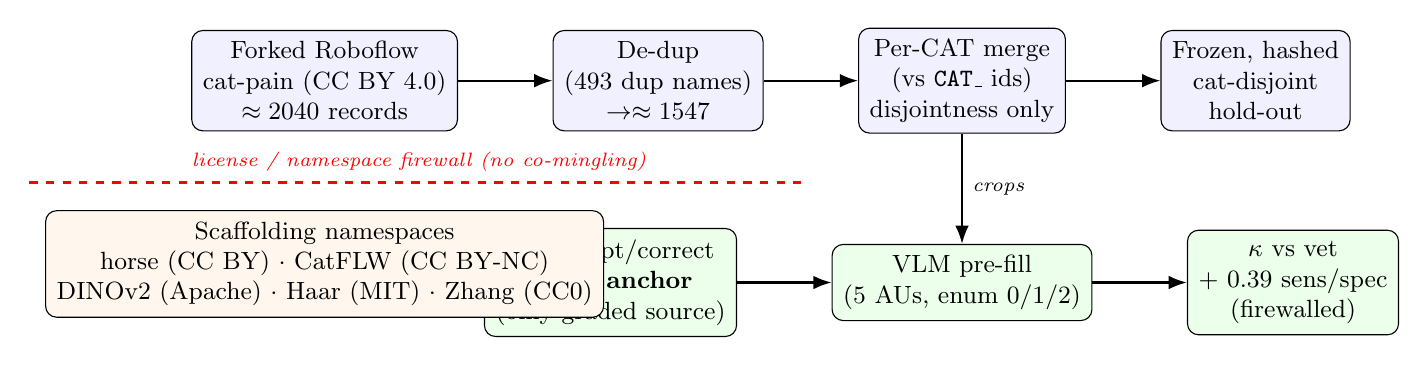
\begin{tikzpicture}[
  node distance=8mm and 12mm,
  box/.style={draw, rounded corners, align=center, font=\small,
              minimum height=8mm, inner sep=4pt, fill=black!3},
  spine/.style={box, fill=blue!6},
  anchorbox/.style={box, fill=green!8},
  scaffold/.style={box, fill=orange!7},
  flow/.style={-{Latex}, thick},
  note/.style={font=\scriptsize\itshape, align=center}
]
% spine pipeline (top row)
\node[spine] (fork)   {Forked Roboflow\\cat-pain (CC BY 4.0)\\$\approx 2040$ records};
\node[spine, right=of fork] (dedup) {De-dup\\($493$ dup names)\\$\rightarrow \approx 1547$};
\node[spine, right=of dedup] (merge) {Per-CAT merge\\(vs \texttt{CAT\_} ids)\\disjointness only};
\node[spine, right=of merge] (holdout) {Frozen, hashed\\cat-disjoint\\hold-out};
% vet anchor branch (bottom)
\node[anchorbox, below=14mm of merge] (vlm) {VLM pre-fill\\(5 AUs, enum $0/1/2$)};
\node[anchorbox, left=of vlm] (vet) {Vet accept/correct\\$=$ \textbf{vet anchor}\\(only graded source)};
\node[anchorbox, right=of vlm] (kappa) {$\kappa$ vs vet\\+ $0.39$ sens/spec\\(firewalled)};
% scaffolding (far left, walled off)
\node[scaffold, below=10mm of fork] (scaff) {Scaffolding namespaces\\
  horse (CC BY) $\cdot$ CatFLW (CC BY-NC)\\
  DINOv2 (Apache) $\cdot$ Haar (MIT) $\cdot$ Zhang (CC0)};
% spine flow
\draw[flow] (fork) -- (dedup);
\draw[flow] (dedup) -- (merge);
\draw[flow] (merge) -- (holdout);
% anchor flow
\draw[flow] (vet) -- (vlm);
\draw[flow] (vlm) -- (kappa);
\draw[flow] (merge) -- node[note, right] {crops} (vlm);
% firewall: scaffolding cannot reach spine
\draw[red, very thick, dashed] ($(scaff.north west)+(-0.2,0.35)$)
   -- ($(scaff.north east)+(2.6,0.35)$)
   node[midway, above, note, text=red] {license / namespace firewall (no co-mingling)};
\end{tikzpicture}
\caption[Data-provenance and namespacing firewall]{Data-provenance and
namespacing firewall. The spine corpus (blue) is de-duplicated, merged per CAT
\emph{only} to assert disjointness, and frozen into a hashed cat-disjoint
hold-out; the vet-anchor branch (green) is the only graded-label source and its
kappa-versus-vet and sensitivity/specificity outputs are firewalled per
Section~\ref{subsec:firewall}; scaffolding sources (orange) are walled in their
own namespaces and never reach a cat-pain loader or a CC~BY release.}
\label{fig:provenance}
\end{figure}

\begin{table}[t]
\centering
\caption[Source inventory and namespacing]{Source inventory: directory, role,
license, and whether the source carries AU labels. Only the vet anchor carries
graded ($0/1/2$) AU labels; only the spine and vet anchor are in the cat-pain
namespace.}
\label{tab:inventory}
\small
\begin{tabular}{@{}p{0.24\linewidth}p{0.21\linewidth}p{0.27\linewidth}p{0.20\linewidth}@{}}
\toprule
\textbf{Source} & \textbf{Role} & \textbf{License} & \textbf{Carries AU labels?} \\
\midrule
Forked Roboflow cat-pain & Binary spine (detector + crop source) & CC~BY~4.0 &
No (binary boxes only) \\
\addlinespace
Vet anchor (size fixed by power gate) & Only graded source (guarded $\kappa$ check; $0.39$ sens/spec estimate, non-reportable at $n_{\text{pos}}{=}16$) &
Project-original (derived) & \textbf{Yes} (per-AU $0/1/2$) \\
\addlinespace
Horse-grimace & Decode unit-test fixture & CC~BY~4.0 &
$3/5$ AUs, $5$ horses (fixture only) \\
\addlinespace
CatFLW & Eye-alignment / NME audit & CC~BY-NC~4.0 &
No ($48$ landmarks, no pain) \\
\addlinespace
\texttt{dinov2-small} & Frozen encoder (plumbing) & Apache-2.0 & n/a \\
\addlinespace
Haar \texttt{frontalcatface} & Fallback cropper / abstention signal & MIT & n/a \\
\addlinespace
Zhang-2008 archive & Fallback aligner (if CatFLW blocked) & CC0 &
No ($9$ coarse landmarks) \\
\bottomrule
\end{tabular}
\end{table}

Finally, Figure~\ref{fig:crops} is a captioned placeholder for the qualitative
crop-acceptance illustration to be produced once the alignment audit has run; no
example images are fabricated here, consistent with the honesty rule that
governs this document.

\begin{figure}[t]
\centering
\fbox{\parbox[c][0.16\textheight][c]{0.86\linewidth}{\centering
\emph{Placeholder --- figure to be produced.}\\[2pt]
Example acceptable (frontal, eye-aligned, sufficient face-pixel resolution)
versus excluded (profile, eyes-closed, occluded, or below the
normalised-mean-error threshold) crops, drawn from the alignment / NME audit of
Section~\ref{subsec:catflw}. Excluded crops are routed to the vet and logged as
abstention signals; no crop images are fabricated in this methodology document.}}
\caption[Acceptable versus excluded crops (placeholder)]{Acceptable versus
excluded face crops (to be produced). The acceptance criterion is the geometric
quality gate of the alignment audit, not pain content.}
\label{fig:crops}
\end{figure}

% Chapter 4 -- Methodology I: Detector, Crop Pipeline, and the Conceded Ordinal Engine
% Self-contained section file: no preamble, no \documentclass.
% Mirrors the template's Chapter 3 (Sec 3.2 Data Preprocessing + Sec 3.3 Modeling).
% HONESTY: no experimental results are reported here. This chapter specifies the
% engineering of the engine and its expected/gate-conditioned behaviour only.

\chapter{Methodology~I: Detector, Crop Pipeline, and the Conceded Ordinal Engine}
\label{ch:methodology-engine}

\section{Scope and a standing concession}
\label{sec:eng-scope}

This chapter specifies the perception \emph{engine} of our system: the binary
pain detector (Phase~A), the face-crop and eye-alignment preprocessing that
feeds it forward, the frozen DINOv2 backbone, the five per-action-unit (per-AU)
ordinal heads, the distributional decode, and the training procedure that fits
the heads. It mirrors the modelling and preprocessing chapter of the reference
template, but it does so under a concession that governs every subsection below
and that we restate without euphemism: \emph{the engine is plumbing, not a
contribution}. The frozen-backbone-plus-ordinal-heads design is a standard,
defensible low-data transfer-learning recipe; we adopt it because it is correct
for our regime, not because it is novel, and we never claim otherwise. The
contribution of this work lives in a portable method built on top of the
engine's outputs: the power-aware, per-AU capture-condition
confound-attribution protocol, which is the headline and is developed in a later
chapter. Supporting it are a guarded VLM-as-AU-rater $\kappa$ reliability check
(inspected-not-validated, with its result pending an independent vet anchor) and
the cited trustworthiness wrapper, which are developed in later chapters.
Everything specified here exists only to
produce calibrated scores for those methods to interrogate.

Two framing commitments follow directly from that concession and recur
throughout the chapter. First, the \emph{validated spine of v1 is binary}: the
per-image pain decision (Section~\ref{sec:eng-detector}) is the only output of
this chapter that is later subjected to a validated sensitivity/specificity
claim, and it is validated on vet-confirmed labels only. Second, the
\emph{graded $0$--$10$ layer ships inspected-not-validated}: the five ordinal
heads, their summed score, and the distributional pmf over that sum
(Sections~\ref{sec:eng-corn}--\ref{sec:eng-decode}) are built, inspected, and
reported qualitatively, but they never enter a validated-claim sentence. The
word ``graded'' is struck from every such sentence by construction, and the
project's headline must hold with the graded layer dropped. We flag the
engineering hooks for this discipline as we reach them.

No numerical results appear in this chapter. Where we state a quantity --- an
expansion margin, an alignment tolerance, an operating point --- it is a
\emph{design value} or a \emph{gate threshold} to be confirmed against
pilot output before freezing, not a measured outcome. Literature figures
(e.g.\ the Feline Grimace Scale validation anchors) are attributed to their
sources and used only to motivate design choices.

Figure~\ref{fig:eng-pipeline} gives the end-to-end view that the remaining
sections fill in.

\begin{figure}[t]
\centering
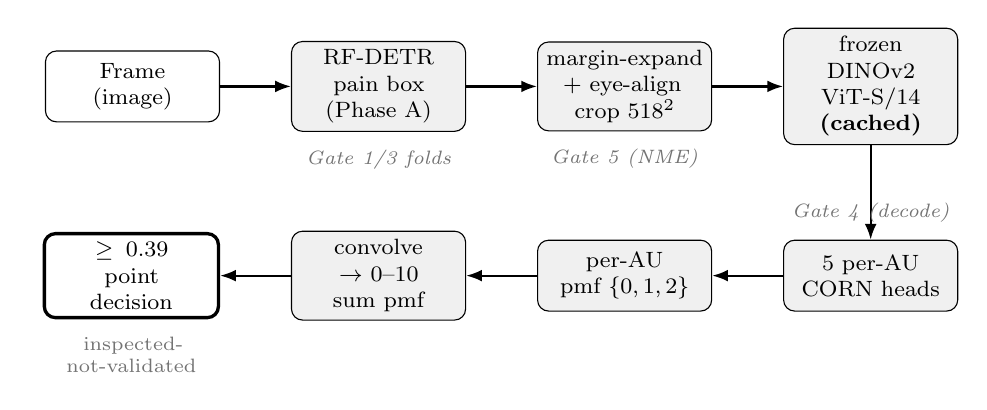
\begin{tikzpicture}[
  node distance=6mm and 9mm,
  box/.style={draw, rounded corners, align=center, minimum height=9mm,
              inner sep=3pt, font=\footnotesize, text width=20mm},
  conc/.style={box, fill=black!6},      % conceded plumbing
  val/.style={box, draw=black, very thick},
  arr/.style={-{Latex[length=2mm]}, thick},
  lbl/.style={font=\scriptsize\itshape, text=black!55}
]
\node[box] (img) {Frame\\(image)};
\node[conc, right=of img] (det) {RF-DETR\\pain box\\(Phase A)};
\node[conc, right=of det] (crop) {margin-expand\\+ eye-align\\crop $518^2$};
\node[conc, right=of crop] (bb) {frozen\\DINOv2\\ViT-S/14\\\textbf{(cached)}};
\node[conc, below=12mm of bb] (heads) {5 per-AU\\CORN heads};
\node[conc, left=of heads] (pmf) {per-AU\\pmf $\{0,1,2\}$};
\node[conc, left=of pmf] (conv) {convolve\\$\rightarrow$ 0--10\\sum pmf};
\node[val, left=of conv] (dec) {$\geq 0.39$\\point\\decision};

\draw[arr] (img) -- (det);
\draw[arr] (det) -- (crop);
\draw[arr] (crop) -- (bb);
\draw[arr] (bb) -- (heads);
\draw[arr] (heads) -- (pmf);
\draw[arr] (pmf) -- (conv);
\draw[arr] (conv) -- (dec);

\node[lbl, below=1mm of det.south] {Gate 1/3 folds};
\node[lbl, below=1mm of crop.south] {Gate 5 (NME)};
\node[lbl, above=1mm of heads.north] {Gate 4 (decode)};
\node[lbl, below=1mm of dec.south, text width=24mm, align=center]
   {\emph{inspected-not-validated}};
\end{tikzpicture}
\caption[End-to-end engine pipeline]{End-to-end engine pipeline. A frame is
localised by the Phase~A detector, the box is margin-expanded and (if Gate~5
requires) eye-aligned into a fixed $518\times518$ crop, encoded once by the
frozen DINOv2 backbone (features cached to disk), and read by five per-AU CORN
heads. Soft per-AU probability mass functions are convolved into a distribution
over the $0$--$10$ sum; a hard decode at the $0.39$ ratio yields the point
decision. Shaded blocks are \emph{conceded plumbing}; the heavy-bordered
decision block and the binary pain decision in Section~\ref{sec:eng-detector}
are the only validated outputs. The $0$--$10$ sum and its pmf ship
inspected-not-validated. Letters in italics mark the gate that governs each
stage.}
\label{fig:eng-pipeline}
\end{figure}

\section{Phase A: the binary pain detector}
\label{sec:eng-detector}

Phase~A is the binary spine of the system and the only stage that produces a
validated number. Its job is twofold: to emit a per-image \emph{pain /
no-pain} decision, and to supply a tight head box that becomes a
\emph{candidate} face crop for the rest of the engine. The decision is the
contribution-bearing output; the crop hand-off is conditional on the alignment
audit of Section~\ref{sec:eng-crop} and is treated as a risk until that audit
passes.

\subsection{Architecture choice}
\label{sec:eng-detector-arch}

We adopt an object-detection formulation rather than a crop-then-classify
pipeline, because the detector doubles as the downstream face cropper and a
separate localiser would be wasted work. The primary architecture is
\textbf{RF-DETR-Nano}, stepping up to RF-DETR-Small only if pain recall
plateaus below target; the runner-up, used as a fallback if RF-DETR training is
unstable on this small, imbalanced corpus, is \textbf{YOLOv11s}. Both are
fine-tuned from COCO-pretrained weights --- the COCO ``cat'' category makes
transfer expected, and we present it as such rather than as a benchmarked
result. The per-image binary decision is the maximum-confidence pain-box score
compared against a tuned threshold (Section~\ref{sec:eng-detector-imbalance});
the DETR-internal transformer backbone is, like the rest of the engine,
conceded plumbing.

\subsection{FGS-safe augmentation}
\label{sec:eng-detector-aug}

The subtle orbital, muzzle, and whisker cues that the Feline Grimace Scale
reads are the entire signal, and any augmentation that distorts facial geometry
poisons both the detector and the crop it produces. We therefore restrict
augmentation to label- and geometry-preserving transforms. Horizontal flip is
permitted (the face is left/right symmetric); small translation and scale and
rotations up to $\sim 10^{\circ}$ are permitted; modest saturation/value jitter
is permitted. Vertical flip is banned outright, because it inverts grimace
geometry; large rotations, heavy colour distortion, and aggressive
mixup/copy-paste \emph{blends} are banned for the same reason. Hue jitter is
held near zero, since coat colour is a capture-condition confound we do not wish
to amplify (the confound itself is audited in a later chapter). Mosaic is
enabled early and disabled for the final epochs so that the last training views
match the real distribution.

\subsection{Imbalance ladder and operating point}
\label{sec:eng-detector-imbalance}

The corpus is heavily imbalanced toward the no-pain class. On the metadata
basis we report throughout --- $264$ pain boxes against $1{,}819$ no-pain boxes,
a prevalence of $\approx 12.7\%$ and an imbalance of $\approx 6.9{:}1$ --- we
note explicitly that these are \emph{box counts, not individual cats}, and that
the live-annotation basis ($246/1{,}811$, $\approx 12.0\%$) is logged as a
discrepancy rather than silently reconciled. We address imbalance with data and
loss before architecture, climbing a fixed ladder and changing one lever per
run, with the decision threshold tuned \emph{last}
(Table~\ref{tab:eng-imbalance}).

\begin{table}[t]
\centering
\footnotesize
\caption[Imbalance ladder for the Phase~A detector]{Imbalance ladder, climbed
cheapest-first; one lever changed per run; the decision threshold moved only
after the data/loss rungs are exhausted. The $\mathrm{pos\_weight}\approx 2.6$
basis is the metadata box ratio $\sqrt{1819/264}$ (box counts, not
individuals); the live-annotation alternative ($\approx 2.7$) is acceptable when
labelled by basis. Values are design defaults, not measured results.}
\label{tab:eng-imbalance}
\begin{tabular}{@{}clll@{}}
\toprule
Rung & Lever & Setting & Fires when \\
\midrule
1 & Class weight / $\mathrm{pos\_weight}$
  & $\sqrt{1819/264}\approx 2.6$ (cap $\sim 3$)
  & always (baseline) \\
2 & Oversample + object copy-paste
  & duplicate pain images; paste pain crops
  & rung-1 recall below target \\
3 & Focal loss
  & $\gamma=1.5,\ \alpha=0.25$
  & rungs 1--2 insufficient \\
4 & Threshold tuning (last)
  & lowest threshold meeting recall $\geq 0.90$
  & only after 1--3 \\
\bottomrule
\end{tabular}
\end{table}

The operating point is fixed at \textbf{pain recall $\geq 0.90$}, selected
inside training folds on the validation precision--recall curve --- explicitly
\emph{not} a Youden-$J$ or $F_1$ knee. A symmetric-cost operating point is the
wrong loss for a welfare instrument in which undertreatment is far costlier than
overtreatment; the welfare-asymmetric decision curve that exploits this choice
is the wrapper's headline artifact and is developed later. The $\geq 0.90$ floor
is justified against the $90.7\%$ reference sensitivity of the Feline Grimace
Scale validation \citep{evangelista2019}, not against prior automated work, and
the specificity it buys is reported with bootstrap confidence intervals across
the five cat-grouped folds. Throughout, augmented and oversampled copies never
enter any reported $N$; every rate is accompanied by the distinct-pain-cat
denominator and Clopper--Pearson or bootstrap intervals, and accuracy and
ROC-AUC are never used as the ranking metric. The primary detection metric is
the precision--recall AUC (average precision) with pain as the positive class.

\subsection{The circularity firewall at the operating point}
\label{sec:eng-detector-firewall}

Phase~A is where the project's central methodological guard first bites. The
sensitivity and specificity reported at the operating point are estimated
\emph{only} on vet-confirmed binary labels. Agreement of any model output
against the VLM-derived weak labels is never treated as validation, because it
would measure the model re-learning the VLM's heuristic rather than tracking
ground truth. This firewall is implemented as a structural constraint on which
label column the evaluation code may read, and it is the reason the binary
decision --- and not the graded sum --- carries the validated claim.

\section{Face-crop and eye-alignment preprocessing (Gate~5)}
\label{sec:eng-crop}

The detector box is a face-crop \emph{candidate}, not a validated cropper. This
section specifies the detect $\rightarrow$ quality-gate $\rightarrow$ expand
$\rightarrow$ align $\rightarrow$ resize pipeline that turns a candidate box
into the fixed crop tensor the backbone consumes, and the blocking Gate~5 audit
that decides whether the cheap box crop suffices or whether a two-point
eye-similarity aligner must be switched on. The motivation is defensive: a
misaligned crop makes any downstream ``calibration'' number a measure of crop
quality rather than of pain, so this stage exists to stop us mistaking one for
the other.

\subsection{Margin expansion}
\label{sec:eng-crop-expand}

The ear AU is read from ear tips and the whisker AU from whisker splay, both of
which sit \emph{outside} a tight head box. We therefore \emph{expand} the box
before cropping rather than shrink it: a $\sim 13.5\%$ margin (midpoint of a
$12$--$15\%$ band), applied asymmetrically with extra room above the head to
recover ear tips. A box already abutting the frame edge cannot be expanded to
recover a clipped ear or whisker; such cases are flagged and routed to the vet
queue as an abstention signal rather than scored on a silently-truncated AU.

\subsection{Frontal-pose and quality gate}
\label{sec:eng-crop-quality}

The Feline Grimace Scale assumes a near-frontal view. Profile, tilted,
occluded, and eyes-closed faces are not scored; they are routed to the vet
queue and never enter the feature cache or any reported denominator. The gate is
a deterministic, training-free, CPU-only filter over the expanded crop: a
yaw/frontality check from the eye-pair geometry, an in-plane tilt check from the
inter-ocular line (the aligner can correct up to $\sim 25^{\circ}$ of roll;
beyond that is a pose problem, not an alignment problem), an eye-aspect-ratio
check for closed eyes, a variance-of-Laplacian blur check, and a coarse Haar
\texttt{frontalcatface} detector whose failure to find a face is itself an
abstention signal. The Haar cascade is used only as a zero-training fallback
localiser and abstention signal --- never as a landmark pipeline, an explicit
avoidance of the landmark-then-geometry trap of prior automated work
\citep{steagall2023}. Each decision and its reasons are written to the crop
manifest; all thresholds are tuned once on the audit set and then frozen, so the
gate cannot be re-tuned to inflate apparent prevalence.

\subsection{The Gate~5 NME audit and the eye-alignment fallback}
\label{sec:eng-crop-gate5}

Gate~5 is blocking: no ordinal head is trained and no vet hour is spent until it
passes. On a small audit set ($30$--$50$ images) it answers two yes/no
questions, using the $48$ CatFLW facial landmarks \citep{martvel2024catflw} as
ground truth. First, is the interocular-normalised mean landmark error (NME)
inside the box crop low enough, and is the box-vs-aligned NME gap small enough,
that the box crop can feed the backbone directly? Second, is the median face
resolution after resize to the backbone's patch grid high enough that AU detail
survives? Design thresholds are a median NME $\leq 0.08$ with a box-vs-aligned
gap $\leq 0.02$, and a median interocular distance $\geq 40$\,px after resize;
these are proposed operating values calibrated to the automated-landmark NME
range of $9$--$26\%$ reported across morphologies by \citet{martvel2024catflw},
to be confirmed against the audit output before freezing. The same work reports
a roughly seven-point pain-accuracy cost from automated versus manual landmarks,
which is precisely the failure mode this gate is built to detect.

If the audit fails, a closed-form \emph{two-point eye-similarity} transform is
switched on as the production crop step: a rotate-plus-uniform-scale-plus-%
translate map taking the two detected eye centres onto fixed canonical targets.
It is a similarity transform with no learned warp and no per-image optimisation,
computed on CPU. Whichever transform Gate~5 certifies --- raw box crop or
eye-aligned crop --- is then frozen and applied once to the full corpus,
producing $518\times518$ RGB crops (with $518 = 14\times 37$ divisible by the
backbone patch size). Crops flagged for the vet queue are excluded from the
feature cache and from every sensitivity/specificity/$\kappa$ denominator,
turning ``detector or quality failure $\rightarrow$ defer to vet'' into an
explicit, counted abstention channel rather than a silent drop.

\section{The frozen DINOv2 ViT-S/14 backbone and feature caching}
\label{sec:eng-backbone}

The encoder is a frozen DINOv2 ViT-S/14 \citep{oquab2023dinov2}: hidden width
$384$, patch size $14$, forward-only. The \emph{register} variant
\texttt{dinov2\_vits14\_reg} is the field default, because registers suppress the
attention artifacts that hurt dense, localized features --- exactly the per-AU
regime (orbital, ear, muzzle); the reg variant is A/B'd against the plain variant
(kept for backwards compatibility) before ViT-S/14 is locked. We freeze it because the supervised set is
on the order of $120$--$300$ vet- and VLM-labelled faces, a regime in which
full fine-tuning of a vision transformer would be malpractice; only the light
ordinal heads are trained. Patch size and hidden width are derived from the
loaded model rather than hard-coded in load-bearing code. The default pooled
representation for the heads is the class token; the mean of the patch tokens is
cached as a second column so that the class-token-versus-mean-patch comparison
is a configuration flag rather than a re-cache.

The single most important engineering decision in this section is
\emph{feature caching}, and it is the decision that makes the whole engine
tractable on an Apple~M4 / MPS machine with no CUDA. Because the backbone is
frozen, its output for a given crop never changes; we therefore run exactly one
forward pass over every crop, write the pooled features to disk, and train the
heads off the cache with \emph{zero} backbone forwards per epoch. This turns
each head epoch from minutes into milliseconds and makes the head sweep
(pooling $\times$ loss $\times$ seeds) a matter of minutes rather than hours.
The DINOv2 commit hash, the preprocessing parameters, the device, and the torch
version are recorded alongside the cache, because the cache is an input to every
reported number. We do \emph{not} domain-adapt the backbone on any external
archive: at this label budget the risk of degrading the features for near-zero
gain is real, and the backbone's generality is what we are relying on.

\section{The five per-AU CORN ordinal heads}
\label{sec:eng-corn}

Each of the five FGS action units --- ear, orbital tightening, muzzle, whiskers,
and head position --- is an ordinal variable on the levels $\{0,1,2\}$. We model
each with a \emph{rank-consistent} ordinal regression head trained with the CORN
(Conditional Ordinal Regression for Neural networks) loss
\citep{shi2023corn}. CORN is chosen over a plain softmax classifier because the
levels are ordered, and over CORAL \citep{cao2020coral} because CORN attains
rank consistency without CORAL's shared-bias capacity restriction. With three
levels per AU, each head emits $K-1 = 2$ conditional logits, so the five AUs
together require a single $384 \rightarrow 10$ linear projection whose output is
split into five two-logit chunks --- one matmul, then a \texttt{split}. The head
is a dropout-regularised linear probe with small-variance truncated-normal
initialisation appropriate to the tiny-data linear-probe regime. The CORN loss
itself is vendored as roughly forty auditable lines (torch and functional only,
no pip dependency) so that the datasheet shows exactly what trained the heads;
it is cross-checked once against a reference implementation in the Gate~4 unit
test (Section~\ref{sec:eng-decode-gate4}) and the reference dependency is then
dropped.

A sibling binary pain head --- a $384 \rightarrow 1$ linear layer trained with a
weighted binary cross-entropy on the pain label --- shares the same cache, is
independent of the CORN heads, and is the v1 spine that the trustworthiness
wrapper actually operates on. The five-AU sum is the inspected path.

The decode contract that turns logits into a level, a sum, and a decision is the
same in this chapter, in the VLM weak-labelling pipeline, and in the wrapper:
the hard level is $\sum_k \mathbb{1}[\operatorname{cumprod}(\sigma(\text{logits}))_k > 0.5]$,
the sum is the sum of the five AU levels in $\{0,\dots,10\}$, and the decision
fires when the ratio $\text{sum}/10$ reaches the clinical cut of $0.39$
(approximately $4/10$) reported by the FGS validation \citep{evangelista2019}.
Crucially the \emph{VLM never emits the sum or the decision}: it emits the five
ordinal atoms, and the sum and the $0.39$ flag are computed in code, so that
there is a single threshold definition in the repository. Figure~\ref{fig:eng-corn}
shows the head and its two decode paths.

\begin{figure}[t]
\centering
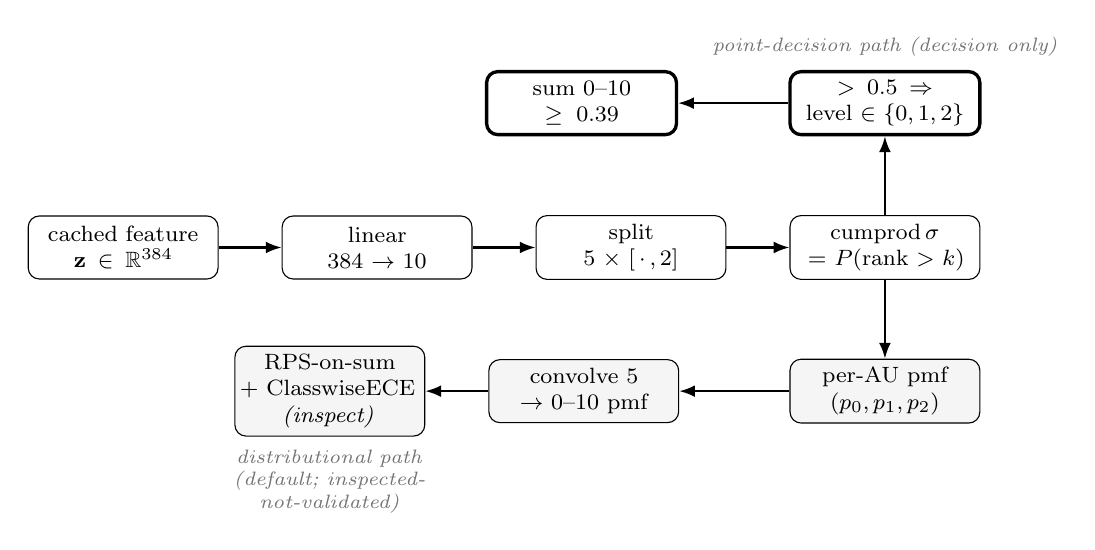
\begin{tikzpicture}[
  node distance=5mm and 8mm,
  box/.style={draw, rounded corners, align=center, minimum height=8mm,
              inner sep=3pt, font=\footnotesize, text width=22mm},
  soft/.style={box, fill=black!4},
  hard/.style={box, draw, very thick},
  arr/.style={-{Latex[length=2mm]}, thick},
  lbl/.style={font=\scriptsize\itshape, text=black!55}
]
\node[box] (feat) {cached feature\\$\mathbf{z}\in\mathbb{R}^{384}$};
\node[box, right=of feat] (proj) {linear\\$384\!\to\!10$};
\node[box, right=of proj] (split) {split\\$5\times[\,\cdot\,,2]$};
\node[box, right=of split] (cum) {$\operatorname{cumprod}\sigma$\\$=P(\text{rank}>k)$};

\node[soft, below=10mm of cum] (pmf) {per-AU pmf\\$(p_0,p_1,p_2)$};
\node[soft, left=14mm of pmf] (conv) {convolve 5\\$\to$ 0--10 pmf};
\node[soft, left=of conv] (rps) {RPS-on-sum\\+ ClasswiseECE\\\emph{(inspect)}};

\node[hard, above=10mm of cum] (thr) {$>0.5 \Rightarrow$\\level $\in\{0,1,2\}$};
\node[hard, left=14mm of thr] (sum) {sum 0--10\\$\geq 0.39$};

\draw[arr] (feat) -- (proj);
\draw[arr] (proj) -- (split);
\draw[arr] (split) -- (cum);
\draw[arr] (cum) -- (pmf);
\draw[arr] (pmf) -- (conv);
\draw[arr] (conv) -- (rps);
\draw[arr] (cum) -- (thr);
\draw[arr] (thr) -- (sum);

\node[lbl, above=0.5mm of thr.north] {point-decision path (decision only)};
\node[lbl, below=0.5mm of rps.south, text width=30mm, align=center]
  {distributional path (default; inspected-not-validated)};
\end{tikzpicture}
\caption[CORN head and distributional decode]{The rank-consistent CORN head and
its two decode paths. A cached feature is projected to five two-logit chunks;
the cumulative product of the sigmoids gives, per AU, $P(\text{rank}>k)$. The
\emph{soft} path (lower, default) turns these into a per-AU pmf and convolves
the five into a distribution over the $0$--$10$ sum, scored by the ranked
probability score and per-AU classwise ECE; this path is inspected, not
validated. The \emph{hard} path (upper) thresholds the cumulative products at
$0.5$ to a level, sums to $0$--$10$, and fires the decision at the $0.39$ ratio.
The hard path is used for the point decision only.}
\label{fig:eng-corn}
\end{figure}

\section{Distributional decode}
\label{sec:eng-decode}

The default scoring path is distributional, not argmax. From each AU's soft
cumulative probabilities $P(\text{rank}>k) = \operatorname{cumprod}(\sigma(\text{logits}))$
we form a proper probability mass function over $\{0,1,2\}$ via
$p_0 = 1 - P(\text{rank}>0)$, $p_1 = P(\text{rank}>0) - P(\text{rank}>1)$, and
$p_2 = P(\text{rank}>1)$, clamping tiny negative values from floating-point
error. The five per-AU pmfs are then \emph{convolved} into a single pmf over the
$0$--$10$ sum. From that distribution we report two things: the ranked
probability score on the sum, as a single scalar with a bootstrap confidence
interval, and a per-AU classwise expected calibration error
\citep{guo2017calibration}. The argmax / hard decode is reserved for the $0.39$
point decision alone.

One reporting decision in this path is load-bearing and we state it explicitly:
\emph{we do not draw a binned reliability diagram on the eleven-atom $0$--$10$
sum}. With only eleven atoms and the label budget we have, per-bin standard
errors are large enough ($\pm 0.18$--$0.26$) that such a diagram would launder
noise as evidence. The ranked probability score on the sum plus per-AU classwise
ECE is the statistically coherent substitute, and it is reported as
inspected-not-validated evidence about the graded layer, never as a validated
calibration claim.

\subsection{Gate~4: blocking decode correctness}
\label{sec:eng-decode-gate4}

Before any score from the engine is believed, two correctness checks must pass,
and they are blocking in continuous integration. The first is a synthetic
decode unit test: hand-verified logit configurations are asserted to decode to
known levels, the decode is asserted monotone in the logits (raising any logit
cannot lower the decoded level, the rank-consistency property), the per-AU pmf
is asserted to sum to one with no negative atoms, the convolved sum pmf is
asserted to be a distribution over $0$--$10$, and the $0.39$ point decision is
asserted at its boundary (a sum of $4$ fires, a sum of $3$ does not). The second
is an MPS-versus-CPU logit-parity check on a real aligned crop, guarding against
silently-wrong accelerator arithmetic --- a leak-proof metric computed from
wrong logits is worthless. A red Gate~4 blocks the entire engine; the vendored
decode is additionally cross-checked once against a reference CORN implementation,
and on disagreement the vendoring is fixed rather than the expected value
adjusted to match a broken decode.

\section{Training: co-teaching small-loss on VLM mass plus a clean vet anchor}
\label{sec:eng-training}

The heads are trained on a mixture of two label sources of very different
quality: a large mass of VLM weak labels covering all scored crops, and a small
clean anchor of vet-confirmed labels (on the order of $120$--$300$ faces, at
least $50$ pain-positive, with the exact integer fixed by the project's power
calculation before any vet hour is spent). Training on the clean anchor alone
gives too few examples; training naively on all labels bakes in the VLM's
under-estimation bias. We therefore use \emph{co-teaching with small-loss
selection}: two heads are trained in parallel, each selecting the small-loss
subset of each mini-batch for its partner, following the canonical Co-teaching
schedule $R(T)=1-\tau\cdot\min(T/T_k,1)$~\cite{han2018coteaching}: the keep-rate
ramps from inclusive toward selective over the first $T_k$ epochs, starting at
$1.0$ (keep all) and descending to $1-\tau$, where $\tau$ is the estimated label
noise rate --- exploiting the memorization effect, whereby networks fit clean
patterns before noisy ones, so noisy examples are pruned late rather than early.
Vet-clean rows are never
dropped from either head's selection --- they are protected anchor points that
the noisy mass is filtered against. AUs left unscored on a given image carry a
sentinel and are skipped in that image's loss, and the weakest AUs (muzzle and
whiskers) may optionally be upweighted. Figure~\ref{fig:eng-coteach} sketches the
scheme.

\begin{figure}[t]
\centering
\fbox{\begin{minipage}{0.92\linewidth}
\centering\footnotesize
\vspace{2mm}
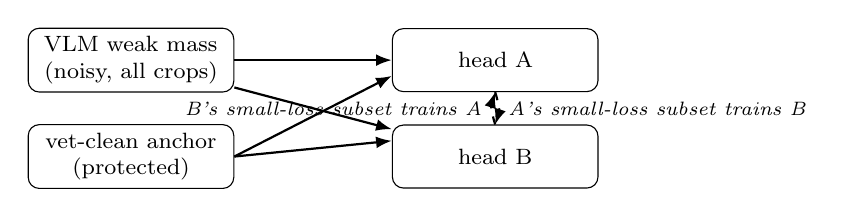
\begin{tikzpicture}[
  node distance=5mm and 10mm,
  blk/.style={draw, rounded corners, align=center, font=\footnotesize,
              minimum height=8mm, inner sep=3pt, text width=24mm},
  arr/.style={-{Latex[length=2mm]}, thick},
  dasharr/.style={-{Latex[length=2mm]}, thick, dashed}
]
\node[blk] (mass) {VLM weak mass\\(noisy, all crops)};
\node[blk, below=4mm of mass] (anchor) {vet-clean anchor\\(protected)};
\node[blk, right=20mm of mass] (A) {head A};
\node[blk, right=20mm of anchor] (B) {head B};
\draw[arr] (mass) -- (A);
\draw[arr] (mass) -- (B);
\draw[arr] (anchor.east) -- ($(A.west)+(0,-2mm)$);
\draw[arr] (anchor.east) -- ($(B.west)+(0,2mm)$);
\draw[dasharr] (A.south) to[bend left=18] node[midway, right, font=\scriptsize\itshape]
   {A's small-loss subset trains B} (B.north);
\draw[dasharr] (B.north) to[bend left=18] node[midway, left, font=\scriptsize\itshape]
   {B's small-loss subset trains A} (A.south);
\end{tikzpicture}
\vspace{1mm}

\emph{Placeholder schematic --- to be replaced by the produced training-loss /
keep-rate figure once runs exist.}
\vspace{2mm}
\end{minipage}}
\caption[Co-teaching small-loss training]{Co-teaching small-loss training. Two
heads consume the same noisy VLM mass; each selects the small-loss subset of a
mini-batch to train its partner, so each head is shielded from the other's
memorised label noise. The vet-clean anchor rows are protected and never
filtered out. Captioned placeholder; no loss curve is shown because no training
run has been performed.}
\label{fig:eng-coteach}
\end{figure}

Folds are cat-disjoint, read from the per-individual merge and the frozen,
hashed hold-out manifest, so that no individual straddles a fold and augmented
copies never enter a reported $N$. The head sweep --- class-token versus
mean-patch pooling, CORN versus CORAL loss, five seeds with mean and bootstrap
CI --- runs in minutes precisely because the backbone never re-runs.

\section{What the engine outputs, and what is and is not claimed}
\label{sec:eng-outputs}

The engine emits the artifacts in Table~\ref{tab:eng-outputs}: cached features,
trained CORN heads, a trained binary pain head, per-AU soft cumulative
probabilities on the hold-out, a convolved $0$--$10$ sum pmf, and the blocking
Gate~4 report. The claim discipline attached to each is the point of this
chapter. The binary pain decision plus abstention is the validated spine, with
sensitivity and specificity estimated downstream on vet-confirmed labels only.
The $0$--$10$ sum is inspected-not-validated: its agreement against the VLM is
never reported as validation, it is discussed qualitatively with the circularity
stated, and the project's abstract holds with it dropped. The engine is never
claimed novel --- a reviewer applying the ``swap the backbone, add some
metrics'' filing finds nothing here to kill, by design. And the kill/pivot rule
is wired in: if the per-AU agreement of the orbital, ear, and head heads against
the vet anchor (gated in a later chapter on the confidence-interval lower bound,
not the point estimate) falls below its pre-registered floor, the graded layer
is dropped entirely and the system ships as a calibrated binary detector with
abstention and the confound audit; the engine's heads still train and ship as
the inspected artifact, but no graded claim is made.

\begin{table}[t]
\centering
\footnotesize
\caption[Phase~B engine outputs and claim status]{Engine outputs and their claim
status. The binary spine is the only validated output; the graded sum and its
pmf are inspected-not-validated; everything else is intermediate plumbing. No
output in this table carries a measured result in this document.}
\label{tab:eng-outputs}
\begin{tabular}{@{}lll@{}}
\toprule
Artifact & Role & Claim status \\
\midrule
Cached frozen features        & input to all heads      & input only \\
Trained CORN heads (5 seeds)  & per-AU ordinal scores   & conceded plumbing \\
Binary pain head              & v1 spine                & \textbf{validated} (vet labels only) \\
Per-AU soft cumulative probs  & feeds wrapper           & intermediate \\
Convolved $0$--$10$ sum pmf   & graded layer            & \emph{inspected-not-validated} \\
Gate~4 decode/parity report   & correctness            & blocking pass/fail \\
\bottomrule
\end{tabular}
\end{table}

In sum, this chapter has specified a deliberately unremarkable engine ---
detector, alignment-gated crop, frozen backbone with cached features,
rank-consistent ordinal heads, distributional decode, and noise-robust training
--- whose every design choice is the conservative one for a low-data,
single-machine, single-vet regime. Its outputs feed the headline confound-attribution
protocol, the guarded VLM-as-AU-rater reliability check, and the cited
trustworthiness wrapper that carry this work's contribution. Nothing here
is offered as novel, and nothing here is reported as a result.

The portable method surface --- the headline capture-condition
confound-attribution protocol and the supporting VLM-as-AU-rater $\kappa$
reliability check --- is dataset-agnostic code in \texttt{src/protocols/}
(with thin adapters for AU override, column mapping, and generic non-FGS ordinal
mode; see \texttt{src/protocols/adapters.py} and re-exports in
\texttt{src/protocols/\_\_init\_\_.py}). The standalone test corpus
(\texttt{src/protocols/standalone\_test\_corpus.py}) exercises the surface on
synthetic arbitrary-AU data with zero torch leakage and is deletion-safe
(imports only the protocols layer); the headline confound leg is additionally
validated today on planted positive and negative controls. The engine remains
conceded plumbing. See also the evaluation protocol
chapter for the gate-enforced usage contract and \texttt{Makefile} targets
\texttt{test-portable} / \texttt{gate-e2e-synthetic}.

The protocols seam (portable pmf derives re-exported del-safe from decode for arbitrary AU via adapters/generic_ordinal_mode; N/k from len/shape, no hard 5/11 in portable path), generalized decode (engine path), DINOv3 prep, and cache schema are the
executable embodiments of portable: use \texttt{src.protocols} adapters +
\texttt{get\_au\_names(override)} + \texttt{generic\_ordinal\_mode} (no 0.39 assumption) for arbitrary ordinal corpora; point-decision
0.39 remains FGS-compat only (single-source in constants). The frozen backbone and feature cache
(\texttt{src/model/backbone.py}, \texttt{src/model/cache\_features.py}) are
DINOv3-ready (SUPPORTED\_VARIANTS includes dinov3\_*; richer patch\_std pooling
per fresh MCP context7 /facebookresearch/dinov3 for localized AU cues; explicit
\_CACHE\_SCHEMA + FEATURE\_SCHEMA with version/n\_aus/k/feature\_dim/patch\_mode
+ full PROVENANCE.json for portable repro across backbones; dinov commit/device/torch
captured). These, with the central orchestrator and standalone exerciser, make the
``portable method'' claim accurate and citable. The engine itself stays
conceded plumbing.

\chapter{Methodology II: VLM Supervision and the Trustworthiness Wrapper (the Headline)}
\label{ch:vlm-wrapper}

The preceding chapter specified the \emph{engine}: a frozen DINOv2 ViT-S/14
backbone feeding five per--action-unit (AU) CORN ordinal heads, decoded to
per-AU levels in $\{0,1,2\}$, summed to a $0$--$10$ Feline Grimace Scale (FGS)
total, and thresholded at the $0.39$ analgesia cut. That engine is conceded
throughout as \emph{plumbing}: it is assembled from standard, off-the-shelf
components and is never claimed as a novel contribution. The present chapter is
where the contribution of this work actually lives. It specifies (i) the
weak-supervision pipeline by which a vision--language model (VLM) produces the
ordinal per-AU labels that the engine consumes, and (ii) the
\emph{trustworthiness wrapper} --- the frame in which the system's outputs are
reported, audited, and gated.

Two of the components below are designated \textbf{portable methods}: they are
dataset-agnostic protocols, released as runnable code, that any future
facial-pain-scoring corpus can re-run. These are the headline deliverables of
the project:

\begin{enumerate}
  \item \textbf{Headline Method 1 --- VLM-as-AU-rater $\kappa$
  (\S\ref{sec:vlm-au-rater-kappa}).} A measurement of whether a frozen VLM can
  weak-label feline FGS action units at human-rater agreement, expressed as five
  per-AU quadratic-weighted kappas against a veterinary anchor, gated on the
  \emph{confidence-interval lower bound} (Gate~1-B).
  \item \textbf{Headline Method 2 --- capture-condition confound-attribution
  protocol (\S\ref{sec:confound-protocol}).} A one-directional audit
  (\emph{FGS-BG-Gap} plus per-AU energy-based pointing game, EBPG) that detects
  whether the scorer is reading acquisition context rather than grimace.
\end{enumerate}

Between these sit the wrapper pillars --- a welfare-asymmetric decision curve, a
fixed-high-sensitivity operating point, and a defer-to-vet abstention boundary
reported as a one-sided lower bound --- which together constitute the clinical
framing that distinguishes this work from a generic pain detector.

\paragraph{Status of this chapter.} This is a methodology and evaluation
protocol. No experiment has yet been run. Every quantitative claim in this
chapter is stated as a \emph{protocol} together with the \emph{decision rule}
(the gate) it feeds; where the literature is cited (e.g.\ Evangelista et al.\ on
human-rater FGS agreement), the numbers are attributed to that source and are
not results of this project. Figures that depend on data not yet collected are
presented as captioned schematic placeholders or as TikZ process diagrams ---
never as plots of invented measurements.

\section{The VLM weak-labeling pipeline}
\label{sec:vlm-pipeline}

The supervision problem is structural. The only in-domain corpus
(\S\ref{ch:datasets}) carries binary \texttt{pain}/\texttt{no\_pain} boxes and
\emph{zero} per-AU or $0$--$10$ FGS labels; no open graded cat-FGS dataset
exists. The five per-AU ordinal targets that the CORN engine requires must
therefore be \emph{manufactured} at low cost and then anchored against a small
veterinary gold set. The weak labeler is a frozen, hosted VLM (Claude),
prompted to emit five FGS action-unit scores per face under a strict,
machine-checkable contract.

\subsection{Forced-tool-use enum schema, rationale-before-score}
\label{sec:vlm-schema}

The VLM is constrained to a single forced tool call. Each of the five AUs is a
nested object whose ordinal level is an \texttt{enum} over $[0,1,2]$ ---
strict structured-output decoding strips numeric \texttt{min}/\texttt{max}
constraints, so an enumeration is the only reliable way to pin the three ordinal
levels. The tool is invoked with
\texttt{tool\_choice=\{"type":"tool",\dots\}} and
\texttt{disable\_parallel\_tool\_use=true} so that exactly one tool-use block is
emitted; \texttt{additionalProperties:false} and an all-\texttt{required} field
set make any contract violation a hard parse failure rather than a silent
mislabel. Within each AU object the \texttt{rationale} field is ordered
\emph{before} the \texttt{score} field, because under tool-use generation the
JSON-schema property order is the token-generation order: the model is forced to
articulate the visible feature before committing to a level. Each AU also
carries a \texttt{confidence} enum (\texttt{low}/\texttt{medium}/\texttt{high})
and an \texttt{abstain} boolean (set when the AU region is occluded, blurred,
out-of-frame, or non-frontal), and the call carries a whole-face
\texttt{image\_quality} enum
(\texttt{frontal\_clear}/\texttt{partial}/\texttt{unusable}).

Crucially, the schema contains \textbf{no \texttt{sum} field, no
\texttt{decision} field, and no \texttt{pain} field}. These quantities are
uncomputable by the VLM \emph{by construction}: the labeler emits five atoms in
$\{0,1,2\}$ and nothing else. The total and the $0.39$ flag are computed in code
(\S\ref{sec:vlm-aggregation}), so the threshold definition has a single source
of truth in the repository and the labeler cannot leak a clinical decision it
was never validated to make.

\begin{figure}[t]
\centering
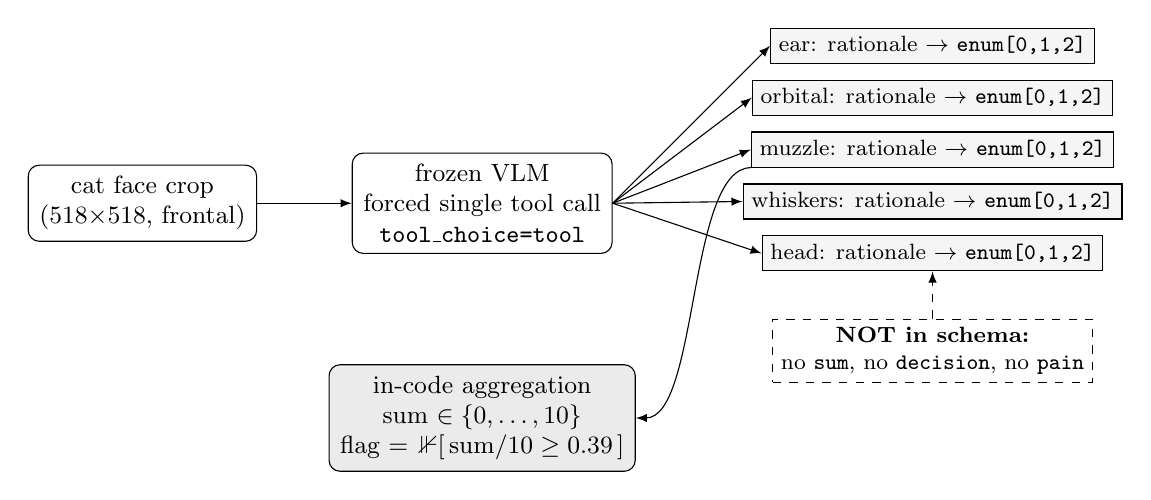
\begin{tikzpicture}[
  node distance=6mm and 12mm,
  box/.style={draw, rounded corners, align=center, inner sep=4pt, font=\small},
  au/.style={draw, align=center, inner sep=3pt, font=\footnotesize, fill=black!4},
  code/.style={draw, rounded corners, align=center, inner sep=4pt, font=\small, fill=black!8},
  ban/.style={draw, dashed, align=center, inner sep=3pt, font=\footnotesize},
  >=latex
]
\node[box] (img) {cat face crop\\(518$\times$518, frontal)};
\node[box, right=of img] (vlm) {frozen VLM\\forced single tool call\\\texttt{tool\_choice=tool}};
\node[au, right=20mm of vlm, yshift=20mm] (ear)   {ear: rationale $\to$ \texttt{enum[0,1,2]}};
\node[au, below=2mm of ear]  (orb)   {orbital: rationale $\to$ \texttt{enum[0,1,2]}};
\node[au, below=2mm of orb]  (muz)   {muzzle: rationale $\to$ \texttt{enum[0,1,2]}};
\node[au, below=2mm of muz]  (whi)   {whiskers: rationale $\to$ \texttt{enum[0,1,2]}};
\node[au, below=2mm of whi]  (hea)   {head: rationale $\to$ \texttt{enum[0,1,2]}};
\node[code, below=14mm of vlm] (agg) {in-code aggregation\\sum $\in\{0,\dots,10\}$\\flag $=\,\mathbb{1}[\,\text{sum}/10\geq 0.39\,]$};
\node[ban, below=6mm of hea] (noban) {\textbf{NOT in schema:}\\no \texttt{sum}, no \texttt{decision}, no \texttt{pain}};

\draw[->] (img) -- (vlm);
\draw[->] (vlm.east) -- (ear.west);
\draw[->] (vlm.east) -- (orb.west);
\draw[->] (vlm.east) -- (muz.west);
\draw[->] (vlm.east) -- (whi.west);
\draw[->] (vlm.east) -- (hea.west);
\draw[->] (muz.south west) .. controls +(left:8mm) and +(right:8mm) .. (agg.east);
\draw[->, dashed] (noban) -- (hea);
\end{tikzpicture}
\caption[Forced-tool-use enum schema]{The forced-tool-use enum schema. The VLM
emits five per-AU records, each \emph{rationale-before-score} over an ordinal
\texttt{enum[0,1,2]}; the $0$--$10$ sum and the $0.39$ analgesia flag are
computed \emph{in code}, never by the VLM. The schema contains no total and no
decision field by construction, so the labeler cannot emit a clinical decision.}
\label{fig:vlm-schema}
\end{figure}

\subsection{The frozen Evangelista rubric in a cached system block}
\label{sec:vlm-rubric}

The scoring rubric is a system block containing one paragraph per AU using the
verbatim Evangelista et al.\ ordinal descriptors~\cite{evangelista2019}
($0=$ absent; $1=$ moderately present or uncertain; $2=$
marked/obvious), with the AU anatomy grounded in CatFACS. The block instructs
the model to \emph{default genuine ambiguity to level~1 with low confidence},
and to set \texttt{abstain} on any occluded, blurred, or non-frontal AU region.
This block is byte-frozen and carried with \texttt{cache\_control} so that the
full corpus run pays for the rubric once; any byte change invalidates the cache,
and the cache hash is pinned in the run configuration for reproducibility (the
run logs \texttt{cache\_read\_input\_tokens}$>0$ to confirm a cache hit). The
frontal-pose and quality gate is thus \emph{inside} the schema rather than a
separate model: \texttt{image\_quality} and per-AU \texttt{abstain} route
non-frontal or occluded crops to the veterinary queue, which the abstention
curve (\S\ref{sec:abstention}) later consumes as a counted channel rather than a
silent drop.

\subsection{Bulk execution: the Message Batches API}
\label{sec:vlm-batch}

The full-corpus weak-labeling run is executed through the Message Batches API
(asynchronous, with a substantial cost discount), sharing the single cached
rubric block across all requests. One request is built per image; a
self-consistency subset is run $N\geq 3$ times at raised temperature to support
the ordinal Krippendorff $\alpha$ axis (\S\ref{sec:vlm-consistency}). The bulk
run is \emph{blocked} until the kappa pilot (Gate~1-B,
\S\ref{sec:vlm-au-rater-kappa}) returns \textsc{go}; on \textsc{no-go} the
project pivots to the binary-plus-wrapper fallback and the kappa numbers ship as
a method finding regardless. All of this section is hosted-API-only --- no local
VLM weights --- so it is identical on the Apple~M4 development machine or any
cloud worker.

\subsection{In-code aggregation: the sum and the $0.39$ flag}
\label{sec:vlm-aggregation}

The five emitted atoms are summed in code to a total $s\in\{0,\dots,10\}$, and
the analgesia flag is $\mathbb{1}[\,s/10 \geq 0.39\,]$ (the Evangelista
$\geq 4/10$ cut~\cite{evangelista2019}). \textbf{This is the identical decode
contract pinned by the engine's blocking Gate~4 unit test}
(decode $\to$ per-AU $0$--$2$ $\to$ sum $\to$ $0.39$): the VLM path and the CORN
path must produce identical sums from identical five-atom inputs, and both
import the same aggregation function, so there is exactly one threshold
definition in the repository. The flag here is \emph{decision-support triage
only}, never an autonomous analgesia trigger, and the sum it rides on is an
\emph{inspected-not-validated} quantity. Following the project-wide honesty
constraint, the word ``graded'' is struck from every validated-claim sentence.

\subsection{Vet-free self-consistency: ordinal Krippendorff $\alpha$}
\label{sec:vlm-consistency}

A vet-free reliability axis runs each image of the self-consistency subset
$N\geq 3$ times at raised temperature and computes the \emph{ordinal}
Krippendorff~$\alpha$~\cite{krippendorff2004} per AU over the
runs-$\times$-items matrix. This serves three purposes: a cheap pre-screen
before any veterinary budget is spent; an abstention signal (low-$\alpha$ AUs
route to vet); and a complement to --- never a replacement for --- the
against-vet kappa of \S\ref{sec:vlm-au-rater-kappa}. Low $\alpha$ on muzzle and
whiskers is anticipated: these are among the weakest AUs even for human experts,
and that expectation feeds both the abstention curve and the per-AU confidence
gating. Self-consistency $\alpha$ is never offered as validation of the $0.39$
flag (\S\ref{sec:firewall}).

\section{Headline Method 1: VLM-as-AU-rater kappa}
\label{sec:vlm-au-rater-kappa}

The first portable contribution is a \emph{measurement}: can a frozen VLM
weak-label feline FGS action units at human-rater agreement? The deliverable is
the \emph{protocol plus result} --- released code that scores any face corpus's
per-AU VLM labels against a veterinary anchor and reports five quadratic kappas
with confidence-interval lower bounds. The numbers obtained on the present
corpus instantiate the protocol; they are not its point. This is the one
fact-about-the-world the project produces, and it is immune to the
``routine hygiene'' critique precisely because no prior feline-pain work has
measured it.

\subsection{The veterinary anchor and the review loop}
\label{sec:vet-anchor}

The anchor is the project's single source of trustworthy per-AU $0/1/2$ labels.
It is not downloaded --- it is \emph{produced} by a prefilled review loop: the
VLM scores each crop with rationale-before-score; the cases that buy the most
information per veterinary hour are triaged to the top (pain-positive and
near-threshold cases with sum $3$--$5/10$; the weakest AUs, muzzle and whiskers;
the most-diagnostic orbital-tightening AU; confident-learning
error flags~\cite{cleanlab2021}; and multi-run VLM disagreements); and the
veterinarian \emph{accepts or corrects} the prefilled scores rather than
labeling from a blank slate. Only vet-confirmed rows enter the kappa
computation. The anchor size is not guessed: it is the single integer fixed by
the Gate~0 power calculation (a $\kappa$ CI half-width target of $\leq 0.15$ via
\texttt{kappaSize}) before any veterinary hour is spent.

\subsection{Per-AU quadratic-weighted kappa, gated on the CI lower bound}
\label{sec:kappa-gate}

For each AU, agreement is the quadratic-weighted Cohen kappa~\cite{cohen1968kappa}
between the VLM level and the vet level, computed row-paired with
\texttt{weights="quadratic"}. The quadratic weighting is what makes the statistic
\emph{ordinal} --- it penalizes a $0$-versus-$2$ disagreement four times as
heavily as a $0$-versus-$1$ disagreement --- and is the difference between a
nominal agreement number and a contribution-grade ordinal one. A one-sided
$95\%$ \emph{lower bound} on each per-AU kappa is obtained by case-resampling
bootstrap (degenerate single-class resamples are skipped).

\paragraph{Gate~1-B fires on the lower bound, not the point estimate.} At the
pilot sample size, a point estimate of $0.60$ is statistically
indistinguishable from a true value of $0.47$; a point-estimate gate is
therefore not a gate at all. The gate is evaluated against the
\emph{confidence-interval lower bound}, with floors that are themselves backed
by a power calculation. Table~\ref{tab:kappa-gate} states the pre-registered
decision rule. The floors shown are the planning defaults that the Gate~0 power
calculation may overwrite; they are never hard-coded in the gate logic.

\begin{table}[t]
\centering
\caption[Gate 1-B per-AU kappa decision rule]{Gate~1-B decision rule. The gate
is evaluated on the one-sided $95\%$ CI \emph{lower bound} of the per-AU
quadratic-weighted kappa, not the point estimate. This is a pre-registered
protocol; no result is asserted here.}
\label{tab:kappa-gate}
\begin{tabular}{@{}lll@{}}
\toprule
Action unit & Floor (gate on CI lower bound) & On failure \\
\midrule
orbital  & $\mathrm{LB} \geq 0.60$ & drop the $0$--$10$ layer; pivot to binary spine \\
ear      & $\mathrm{LB} \geq 0.60$ & (same) \\
head     & $\mathrm{LB} \geq 0.60$ & (same) \\
muzzle   & $0.40$--$0.60$ acceptable-with-caveat; $<0.40 \to$ drop this AU's head & proceed on surviving AUs \\
whiskers & $0.40$--$0.60$ acceptable-with-caveat; $<0.40 \to$ drop this AU's head & proceed on surviving AUs \\
\bottomrule
\end{tabular}
\end{table}

\paragraph{The pilot self-justifies the labeler.} The choice of VLM is settled
by this pilot --- each candidate model is run and the one with the higher per-AU
kappa lower bounds is selected --- and \emph{no external citation} is invoked to
justify the labeler. This deliberately removes a phantom-citation dependency at
the root of the headline. A \textsc{no-go} on orbital/ear/head is a
\emph{pivot}, not a kill: the project drops the $0$--$10$ layer and ships the
calibrated binary spine plus abstention plus the confound protocol, and a
mediocre-but-first per-AU kappa remains a publishable method finding in its own
right.

\section{The circularity firewall}
\label{sec:firewall}

The single most load-bearing methodological commitment of the project is a
firewall that separates \emph{validation} from \emph{agreement measurement}. It
is stated in code comments and in the paper, and it governs which numbers may
appear in which tables.

\begin{itemize}
  \item \textbf{Sensitivity and specificity at $0.39$ are estimated only on
  vet-confirmed labels.} These are the validated spine numbers, reported with
  Clopper--Pearson or bootstrap intervals and the distinct-pain-cat denominator.
  \item \textbf{Quadratic-weighted kappa against the VLM is never validation.}
  The per-AU kappa of \S\ref{sec:vlm-au-rater-kappa} measures VLM-versus-vet
  agreement --- a forward-looking method finding. It is not evidence that the
  $0.39$ flag is clinically correct.
  \item \textbf{A kappa computed against VLM-derived labels is forbidden as a
  validation metric}, because it would measure only the model re-learning the
  VLM's heuristic.
  \item \textbf{The graded-sum kappa is an internal inspection metric only.} The
  $0$--$10$ artifact ships inspected-not-validated, and no binned reliability
  diagram is ever drawn on the $11$-atom sum.
\end{itemize}

\begin{figure}[t]
\centering
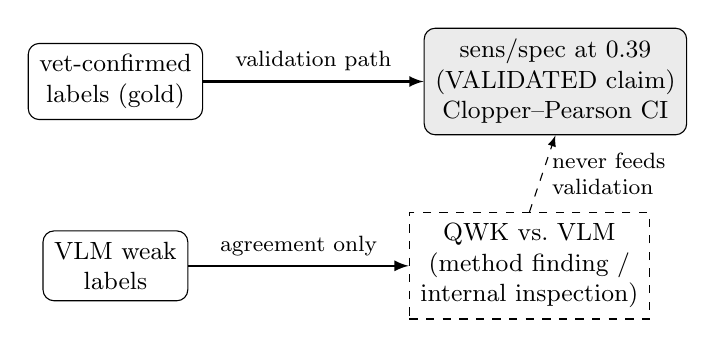
\begin{tikzpicture}[
  node distance=8mm and 16mm,
  src/.style={draw, rounded corners, align=center, inner sep=4pt, font=\small},
  valid/.style={draw, rounded corners, align=center, inner sep=4pt, font=\small, fill=black!8},
  excl/.style={draw, dashed, align=center, inner sep=4pt, font=\small},
  >=latex
]
\node[src] (vet)  {vet-confirmed\\labels (gold)};
\node[src, below=14mm of vet] (vlm)  {VLM weak\\labels};
\node[valid, right=28mm of vet] (sens) {sens/spec at $0.39$\\(VALIDATED claim)\\Clopper--Pearson CI};
\node[excl, right=28mm of vlm] (qwk)  {QWK vs.\ VLM\\(method finding /\\internal inspection)};

\draw[->, thick] (vet) -- node[above, font=\footnotesize] {validation path} (sens);
\draw[->, thick] (vlm) -- node[above, font=\footnotesize] {agreement only} (qwk);
\draw[->, dashed] (qwk.north) -- node[right, font=\footnotesize, align=left]
  {never feeds\\validation} (sens.south);
\end{tikzpicture}
\caption[Circularity firewall]{The circularity firewall. Validated sensitivity
and specificity at the $0.39$ cut are estimated \emph{only} on vet-confirmed
labels (solid path). The quadratic-weighted kappa against VLM labels is a
forward-looking method finding and an internal inspection metric; it never feeds
the validation path (dashed, excluded). This separation is what prevents the
system from validating itself on its own weak supervision.}
\label{fig:firewall}
\end{figure}

\section{Wrapper Pillar: the welfare-asymmetric decision curve}
\label{sec:decision-curve}

The wrapper's headline artifact is \emph{not} a calibration plot but a
welfare-asymmetric decision curve. Pain assessment is a cost-asymmetric
decision: failing to treat a painful cat (undertreatment) is a different and
generally heavier harm than treating a comfortable one (overtreatment). A
symmetric-cost operating point --- the Youden-$J$ knee or an $F_1$ optimum ---
is the wrong loss for a welfare instrument. Decision-curve analysis
\cite{vickers2006dca} reframes the question as net benefit across a
threshold-probability axis, where the threshold probability $p_t$ encodes the
harm ratio via $p_t = \text{overtreat} / (\text{undertreat} + \text{overtreat})$.

Because no veterinarian-elicited harm ratio is available, the undertreat-to-overtreat
ratio is never pinned to a single value: it is \emph{swept as a range} across
the threshold-probability axis. The deliverable is the curve itself, computed
with the \texttt{dcurves} implementation of net benefit, with the fixed-recall
operating point (\S\ref{sec:operating-point}) annotated on it and a
cat-grouped bootstrap ribbon for the confidence band. The claim the curve
supports is that the model's net benefit exceeds both \emph{treat-all} and
\emph{treat-none} across the welfare-relevant low-$p_t$ band; this is a
clinical-decision-theory contribution that no prior cat-pain paper has made, and
it is the floor that survives every downstream null. If the abstention power
budget fails (Gate~0), this pillar becomes the primary clinical deliverable.

\begin{figure}[t]
\centering
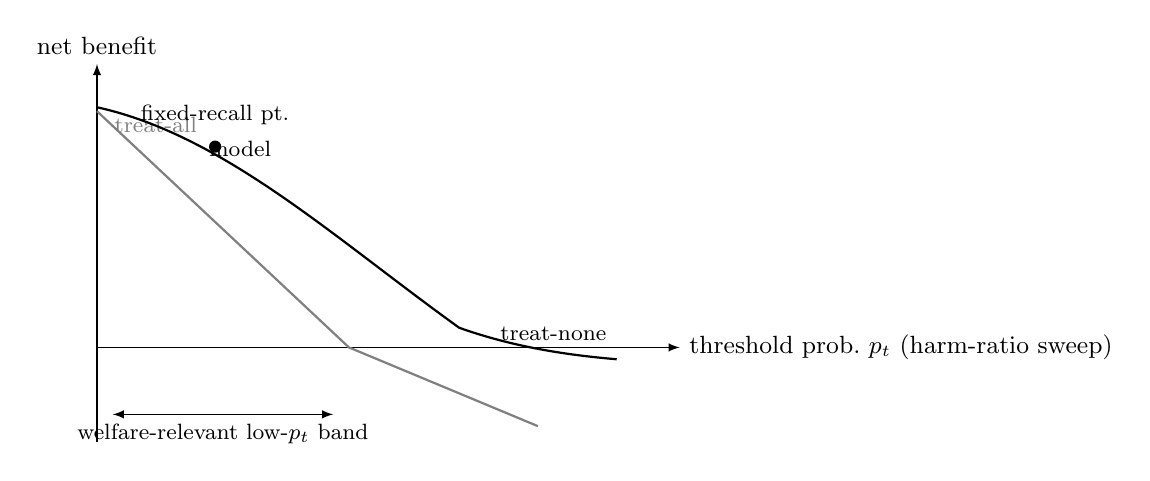
\begin{tikzpicture}[>=latex, font=\small]
% schematic axes only --- NO DATA
\draw[->] (0,0) -- (7.4,0) node[right] {threshold prob.\ $p_t$ (harm-ratio sweep)};
\draw[->] (0,-1.2) -- (0,3.6) node[above] {net benefit};
\draw[dashed] (0,0) -- (7.2,0);
% treat-none baseline (zero net benefit)
\node[font=\footnotesize, anchor=west] at (5.0,0.18) {treat-none};
% treat-all line: high at low pt, crosses to negative
\draw[thick, gray] (0,3.0) -- (3.2,0) -- (5.6,-1.0);
\node[font=\footnotesize, gray, anchor=south west] at (0.1,2.6) {treat-all};
% model curve: dominates over a low-pt band
\draw[thick] (0,3.05) .. controls (1.6,2.7) and (3.0,1.4) .. (4.6,0.25)
  .. controls (5.3,0.0) and (6.0,-0.1) .. (6.6,-0.15);
\node[font=\footnotesize, anchor=south west] at (1.3,2.3) {model};
% annotated fixed-recall point
\fill (1.5,2.55) circle (2.2pt);
\node[font=\footnotesize, anchor=south] at (1.5,2.7) {fixed-recall pt.};
% welfare-relevant band shading marker
\draw[<->] (0.2,-0.85) -- (3.0,-0.85)
  node[midway, below, font=\footnotesize] {welfare-relevant low-$p_t$ band};
\end{tikzpicture}
\caption[Welfare-asymmetric decision curve (schematic)]{\textsc{Schematic
placeholder --- axes and qualitative shape only, no data.} The welfare-asymmetric
decision curve: net benefit versus threshold probability $p_t$, where $p_t$
sweeps the undertreat\,:\,overtreat harm ratio as a range. The headline claim is
that the model curve dominates both treat-all and treat-none across the
welfare-relevant low-$p_t$ band; the fixed-recall operating point is annotated.
The actual curve is to be produced from vet-confirmed held-out scores.}
\label{fig:decision-curve}
\end{figure}

\section{Wrapper Pillar: the fixed pain-recall operating point}
\label{sec:operating-point}

The decision threshold is selected at a \emph{fixed pain-recall} of
$\geq 0.90$ --- the Evangelista sensitivity anchor~\cite{evangelista2019} ---
rather than at a Youden-$J$ or $F_1$ optimum. The selection is performed inside
the training folds only, and the specificity it buys is reported with bootstrap
confidence intervals on out-of-fold predictions. Fixing recall first is the
direct consequence of the welfare asymmetry of \S\ref{sec:decision-curve}: the
dominant cost is missed pain, so the operating point is pinned to control that
miss rate and the specificity cost is reported honestly rather than optimized
against an inappropriate symmetric criterion. This choice corrects the stale
symmetric-knee default and ties the operating point to a clinically meaningful
target. The relevance of a fixed-recall operating point in low-prevalence
settings is sharpened by measurement-error propagation analyses, which show that
modest per-rating error can collapse effective sensitivity when prevalence is
low~\cite{chavoshi2025}; this motivates both the high-recall pin and the
abstention channel of \S\ref{sec:abstention}.

\section{Wrapper Pillar: defer-to-vet abstention as a one-sided NPV lower bound}
\label{sec:abstention}

The abstention pillar reports a defer-to-vet boundary. Around the fixed $0.39$
point, two thresholds $\lambda_1 < \lambda_2$ define a band: confident
no-pain below $\lambda_1$, confident pain above $\lambda_2$, and a deferred
middle band routed to the veterinarian. The reported quantity is the
\emph{negative predictive value} (NPV) --- the dominant clinical cost is a
missed painful cat --- as a function of the abstention rate, and it is reported
as a \textbf{one-sided $95\%$ lower bound at each abstention rate}.

\paragraph{The word ``guaranteed'' is banned.} The lower bound is obtained by a
distribution-free, finite-sample risk-control procedure (Learn-then-Test
\cite{angelopoulos2021ltt}), which controls the NPV risk function at confidence
$\delta = 0.05$ for a tolerated risk $\alpha = 1 - \text{target NPV}$. Because
this is a finite-sample lower bound and not a certainty, the project reports
``NPV with a one-sided $95\%$ lower bound,'' and the word ``guaranteed'' never
appears. Whether a useful band is even certifiable is itself decided by a Gate~0
power calculation \emph{before} any veterinary spend: if the budget cannot
certify NPV $\geq 0.90$ at $\leq 40\%$ abstention, the curve ships
\emph{exploratory-only} and the clinical deliverable relocates to the decision
curve of \S\ref{sec:decision-curve}. This is a demotion, not a kill.

\begin{figure}[t]
\centering
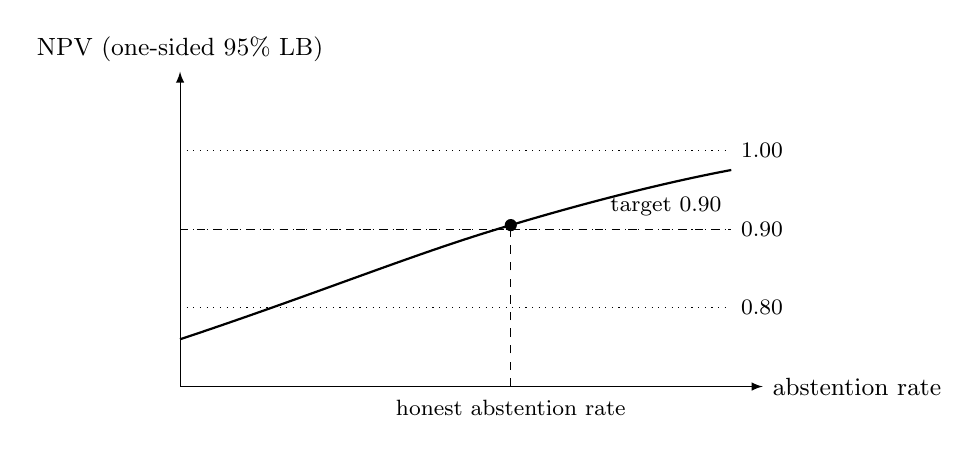
\begin{tikzpicture}[>=latex, font=\small]
% schematic axes only --- NO DATA
\draw[->] (0,0) -- (7.4,0) node[right] {abstention rate};
\draw[->] (0,0) -- (0,4.0) node[above] {NPV (one-sided $95\%$ LB)};
\foreach \y/\l in {1.0/0.80, 2.0/0.90, 3.0/1.00}
  \draw[dotted] (0,\y) -- (7.0,\y) node[right, font=\footnotesize] {\l};
% target line at 0.90
\draw[dashed] (0,2.0) -- (7.0,2.0);
\node[font=\footnotesize, anchor=south east] at (7.0,2.05) {target $0.90$};
% monotone-ish increasing LB curve crossing 0.90 at some honest abstention rate
\draw[thick] (0,0.6) .. controls (1.8,1.2) and (3.0,1.7) .. (4.2,2.05)
  .. controls (5.2,2.35) and (6.2,2.6) .. (7.0,2.75);
% crossing marker
\fill (4.2,2.05) circle (2.2pt);
\draw[dashed] (4.2,0) -- (4.2,2.05);
\node[font=\footnotesize, anchor=north] at (4.2,-0.05) {honest abstention rate};
\end{tikzpicture}
\caption[One-sided NPV lower bound vs.\ abstention rate (schematic)]{\textsc{Schematic
placeholder --- axes and qualitative shape only, no data.} The defer-to-vet
abstention curve: the one-sided $95\%$ NPV lower bound rises with the abstention
rate and clears the $0.90$ target only at an honestly-reported abstention rate.
``Guaranteed'' is never used; the bound is exploratory if the Gate~0 power
budget is unmet. The actual curve is to be produced from vet-confirmed held-out
scores.}
\label{fig:abstention}
\end{figure}

\section{Headline Method 2: the confound-attribution protocol}
\label{sec:confound-protocol}

The second portable contribution is a capture-condition confound-attribution
protocol: a reusable, one-directional audit that any future facial-pain-scorer
corpus can run to ask whether the scorer is reading acquisition context --- the
cage, the clinic, the lighting --- rather than the grimace itself. Single-source
data makes this audit essential: pain and capture condition are plausibly
entangled, and a scorer that exploits that entanglement would post strong
accuracy while learning nothing about pain. The deliverable is the
\emph{protocol}, released as code, not a verdict about this particular corpus.

\paragraph{One-directional by construction.} The audit is well-powered to
\emph{detect} confounding but underpowered to \emph{rule it out}. Every report
therefore reads ``no confound detected at this power'' --- never ``no
confound.'' This asymmetry is stated as a fixed property of the method, not a
caveat appended after the fact.

The protocol has two components, summarized in Figure~\ref{fig:confound}.

\paragraph{(a) FGS-BG-Gap --- the background counterfactual.} The cat face is
masked (training-free, via DINOv2 attention rollout, a segment-anything mask, or
grabcut) and composited onto (i) a same-condition and (ii) a \emph{swapped}
clinic background; the score shift is measured. FGS-BG-Gap is reported as the
mean $0$--$10$ shift plus the pain-flip rate, per AU, stratified by capture
condition. A large gap on a specific AU indicates that head is reading the
cage or clinic rather than the cat. This component adapts the
background-robustness counterfactual framework~\cite{xiao2021background} to the
FGS setting.

\paragraph{(b) Per-AU EBPG --- the energy-based pointing game.} Per-AU saliency
(attention rollout or Score-CAM~\cite{wang2020scorecam} on the frozen backbone)
is scored against an anatomical region of interest derived from CatFLW
landmarks: the protocol reports $\text{energy-in-ROI} / \text{energy-whole}$ per
AU, stratified by capture condition. This answers the question ``does the ear
head fire on the ear?'' --- a per-AU localization-faithfulness measurement that
no prior cat-pain work reports. Where landmark coverage is partial, EBPG is
reported only on the covered subset with the denominator stated.

\begin{figure}[t]
\centering
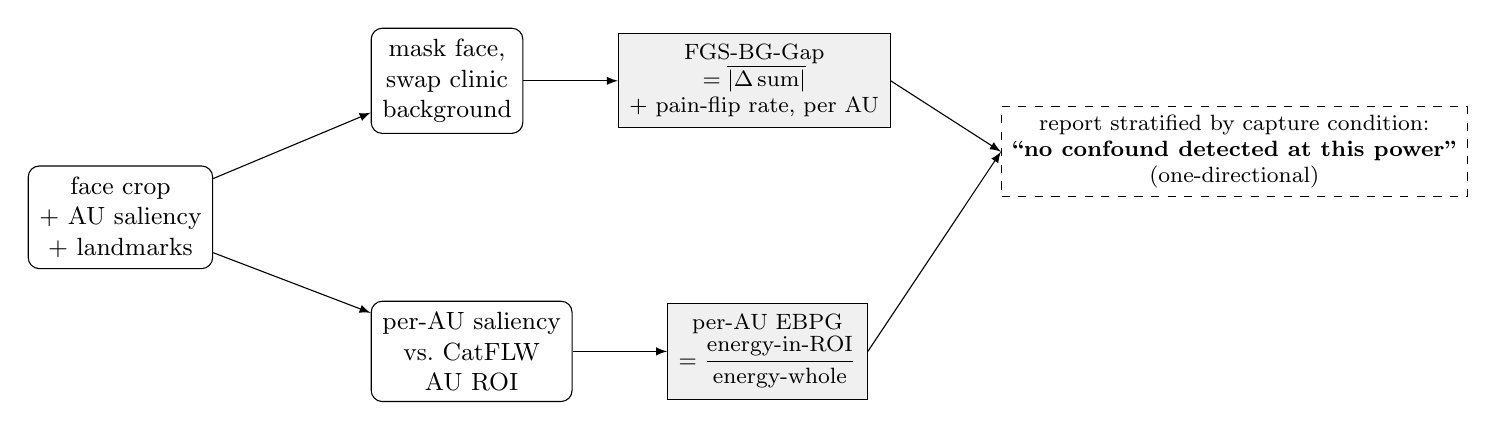
\begin{tikzpicture}[
  node distance=6mm and 12mm,
  box/.style={draw, rounded corners, align=center, inner sep=4pt, font=\small},
  outbox/.style={draw, align=center, inner sep=4pt, font=\footnotesize, fill=black!6},
  oned/.style={draw, dashed, align=center, inner sep=3pt, font=\footnotesize},
  >=latex
]
\node[box] (face) {face crop\\+ AU saliency\\+ landmarks};
% branch A
\node[box, above right=4mm and 20mm of face] (mask) {mask face,\\swap clinic\\background};
\node[outbox, right=of mask] (bggap) {FGS-BG-Gap\\$=\overline{|\Delta\,\text{sum}|}$\\+ pain-flip rate, per AU};
% branch B
\node[box, below right=4mm and 20mm of face] (sal) {per-AU saliency\\vs.\ CatFLW\\AU ROI};
\node[outbox, right=of sal] (ebpg) {per-AU EBPG\\$=\dfrac{\text{energy-in-ROI}}{\text{energy-whole}}$};
\node[oned, right=14mm of bggap, yshift=-9mm] (report)
  {report stratified by capture condition:\\\textbf{``no confound detected at this power''}\\(one-directional)};

\draw[->] (face) -- (mask);
\draw[->] (face) -- (sal);
\draw[->] (mask) -- (bggap);
\draw[->] (sal) -- (ebpg);
\draw[->] (bggap.east) -- (report.west);
\draw[->] (ebpg.east) -- (report.west);
\end{tikzpicture}
\caption[Confound-attribution protocol]{The capture-condition
confound-attribution protocol (Headline Method~2), portable and
one-directional. Branch (a) FGS-BG-Gap measures the score shift under a swapped
clinic background; branch (b) per-AU EBPG measures whether each AU head's
saliency falls inside its anatomical ROI. Both are stratified by capture
condition and reported as ``no confound detected at this power.'' The deliverable
is the protocol, not a verdict on any single corpus.}
\label{fig:confound}
\end{figure}

\section{Where calibration sits: supporting evidence, never headline}
\label{sec:calibration-supporting}

For completeness, the $0$--$10$ layer's reliability is examined through the
distributional decode path of the engine (soft cumulative probabilities $\to$
per-AU probability mass functions $\to$ convolution to a $0$--$10$ sum pmf),
yielding a ranked probability score on the sum and per-AU classwise expected
calibration error~\cite{guo2017calibration}. These calibration quantities are
\emph{supporting evidence only}. They are never a headline; no binned
reliability diagram is drawn on the degenerate $11$-atom sum; and they never
substitute for the welfare-asymmetric decision curve of
\S\ref{sec:decision-curve}, which remains the headline wrapper artifact. This
keeps the contribution clearly located in the two portable methods and the
welfare framing, with generic calibration relegated to hygiene.

\section{Summary}
\label{sec:ch5-summary}

This chapter specified the supervision and trustworthiness layers that carry the
project's contribution. The VLM weak-labeler emits five rationale-before-score
ordinal atoms under a forced-tool-use enum contract, with the sum and the $0.39$
flag computed in code so the labeler never makes a clinical decision. Headline
Method~1 measures per-AU VLM-versus-vet quadratic-weighted kappa, gated on the
CI lower bound; Headline Method~2 is a one-directional, portable
confound-attribution protocol. Between them, a welfare-asymmetric decision
curve, a fixed pain-recall operating point, and a one-sided NPV-lower-bound
abstention boundary constitute the clinical frame, while the circularity
firewall ensures that validation rides on vet-confirmed labels only and that
agreement-against-VLM is never mistaken for validation. The engine remains
conceded plumbing; the contribution lives here, and every claim in this chapter
is stated as a protocol and a decision rule, not as a result.

\chapter{Evaluation Protocol and Gate System}
\label{ch:eval-protocol}

This chapter specifies \emph{how} the system of
Chapters~\ref{ch:methodology-engine} and~\ref{ch:vlm-wrapper} will be
evaluated and \emph{in what order} its components are permitted to run. It is a protocol
chapter, not a results chapter: no experiment has been executed at the time of writing, and
consequently no accuracy, kappa, calibration, or net-benefit number from \emph{our} system
appears anywhere below. Every quantitative figure cited in this chapter is either (i) a
\emph{target} or \emph{pre-registered floor} drawn from the build plan, or (ii) a published
number from the prior literature, attributed to its source. The chapter is organised around a
single conviction inherited from the project's design debate: that the credibility of a
low-data, single-source feline-pain instrument is determined less by any headline metric than
by the \emph{discipline} of the procedure that produces it. We therefore present the
cross-validation and frozen hold-out design (\S\ref{sec:cv-holdout}), the Phase~A and Phase~B
metric definitions (\S\ref{sec:phaseA-metrics}--\S\ref{sec:phaseB-metrics}), the blocking gate
checklist $G0\ldots G6$ plus $G1\text{-}B$ (\S\ref{sec:gates}), the reproducibility contract
(\S\ref{sec:repro}), and the anti-benchmark reporting rules (\S\ref{sec:anti-benchmark}) as a
single, executable evaluation contract.

A note on terminology used throughout. The instrument's \emph{validated} claims concern the
binary pain decision and the two portable methods (the per-action-unit (AU) VLM-as-rater
$\kappa$ protocol and the capture-condition confound-attribution protocol). The graded
$0\text{--}10$ Feline Grimace Scale (FGS) sum is reported as an
\emph{inspected-not-validated} artifact; wherever a metric is computed on the graded sum, it is
labelled inspection-only and is never advanced as evidence for a validated claim.

\section{Cross-validation and the frozen hold-out}
\label{sec:cv-holdout}

\subsection{Grouped stratified cross-validation}

The corpus is the forked Roboflow \texttt{cat-pain} binary detection dataset
($\approx 2040$ records, $\approx 1547$ distinct after collapsing $493$ exact-duplicate
filenames, $336$ source clips, pain prevalence $\approx 12.7\%$). Because the dataset is
small, class-imbalanced, and contains many frames drawn from a handful of source clips and
individuals, the dominant statistical risk is \emph{subject leakage}: near-identical frames of
the same animal appearing in both a training and an evaluation partition would inflate every
reported metric. The evaluation therefore uses subject-exclusive cross-validation.

Folds are produced by \texttt{StratifiedGroupKFold} with $5$ splits, stratified on the
image-level binary pain label and grouped by \emph{individual} (\texttt{cat\_id}). Image-level
(not clip-level) stratification is mandatory because $135$ of the $336$ clips are class-mixed
and cannot be collapsed to a single label without discarding information. Grouping by the
individual---never by clip---is required for leakage safety: letting one individual's frames
straddle folds is the same-subject leakage that subject-exclusive (leave-one-animal-out)
validation exists to prevent, the named standard in this subdomain~\cite{feighelstein2023}. The
one complication is the most prolific known individual (\texttt{CAT\_01}, $84$ clips,
$\approx 605$ images, $\approx 30\%$ of the corpus): grouping it naively into the folds would
fuse a single degenerate super-group fold (\texttt{StratifiedGroupKFold} degrades to
\texttt{GroupKFold} for a dominant group). We therefore \emph{carve \texttt{CAT\_01} out as a
frozen leave-one-individual-out hold-out} and run \texttt{StratifiedGroupKFold(groups=cat\_id)}
over the remaining individuals only---leakage-safe \emph{and} balanced---reporting
\texttt{CAT\_01} performance separately via that hold-out. The splitter is shared verbatim by
Phase~A and Phase~B so that the partition boundaries never shift between the two evaluation
regimes:

\begin{verbatim}
from sklearn.model_selection import StratifiedGroupKFold
m = (cat_id != "CAT_01")            # CAT_01 -> frozen leave-one-individual-out hold-out, never in CV
sgkf = StratifiedGroupKFold(n_splits=5, shuffle=True, random_state=42)
for tr, va in sgkf.split(X=images[m], y=labels[m], groups=cat_id[m]):
    assert set(cat_id[m][tr]).isdisjoint(set(cat_id[m][va]))   # G1 disjointness (per individual)
    assert "CAT_01" not in set(cat_id[m][va])                  # dominant individual excluded from CV
    pf = labels[m][va].mean()
    assert abs(pf - 0.127) <= 0.05 and labels[m][va].sum() >= 25  # per-fold prevalence + count
\end{verbatim}

The per-fold disjointness assertion is a hard runtime check, not a comment: a violation aborts
the run. The per-fold positive counts are recomputed after carving out \texttt{CAT\_01} and
grouping by individual; the gate requires that no fold falls at zero or one positive, so that
subject-exclusive cross-validation remains feasible without empty strata. All preprocessing, threshold selection, temperature scaling, and abstention calibration
are fit \emph{inside each training fold only} (nested); the validation fold sees only frozen,
already-fit transforms. Out-of-fold predictions are pooled, and every reported rate is
accompanied by its bootstrap $95\%$ confidence interval, with the interval \emph{width} stated
up front rather than buried.

\subsection{The frozen, hashed, cat-disjoint hold-out (Gate~3)}

Cross-validation alone does not defend against post-hoc goalpost-moving --- the temptation to
re-select a test partition after seeing results. We therefore carve out a single
boundary-rich, true-prevalence ($\approx 13\%$) test set from cat-disjoint merged groups
\emph{before} cross-validation begins, and freeze it. The test manifest --- the list of test
group identifiers together with the SHA-256 of the fold CSV --- is itself hashed, and the hash
is committed to the repository:

\begin{verbatim}
manifest = {"version": "<roboflow_version>",
            "test_groups": sorted(test_group_ids),
            "fold_csv_sha256": sha256(folds.csv)}
manifest_hash = sha256(json.dumps(manifest, sort_keys=True))
\end{verbatim}

A continuous-integration (CI) guard then \emph{aborts any training, sweep, or
threshold-tuning run that can read the test manifest}, and the hold-out evaluation script
refuses to run if the working tree's fold CSV was mutated after the freeze. This converts the
discipline of ``never look at the test set during selection'' from a promise into an enforced
structural property: the only code path that may read the hold-out is the final evaluation,
executed once. This is the \emph{CI-abort} contract of Gate~3.

\subsection{Honest denominators and confidence intervals}

Three reporting rules apply to \emph{every} rate in the document and are restated here because
they are the substance of the cross-validation design, not decoration:

\begin{enumerate}
  \item \textbf{The distinct-pain-cat denominator is always printed.} A sensitivity reported
        over frames is meaningless if those frames are many views of few animals; the count of
        distinct pain-positive individuals is therefore printed alongside every pain-class rate.
  \item \textbf{Augmented copies never enter any reported $N$.} Geometric or photometric
        augmentation is a training-time device only; no augmented image contributes to a
        denominator, a numerator, or a confidence interval.
  \item \textbf{Every proportion carries an interval.} Proportions are reported with
        Clopper--Pearson exact intervals; pooled and derived statistics (PR-AUC, $\kappa$,
        RPS, net benefit) carry cat-grouped bootstrap $95\%$ intervals.
\end{enumerate}

The headline cross-validation is the multi-frame, per-cat-grouped design with honestly wide
intervals and per-clip inference aggregation. A one-frame-per-cat secondary clean hold-out is
reported \emph{only if} the merged distinct-pain-cat count remains above $50$; otherwise it is
omitted rather than reported on a denominator too small to interpret.

\section{Phase~A metrics: the binary spine}
\label{sec:phaseA-metrics}

Phase~A evaluates the binary pain detector (Chapter~\ref{ch:methodology-engine}) that constitutes
the validated spine of the instrument. The class imbalance ($\approx 13\%$ positive) makes
two conventional choices actively misleading and both are prohibited: accuracy (dominated by
the majority class) and ROC-AUC (whose specificity axis is insensitive at low prevalence) are
never used to rank models.

The \textbf{primary} ranking metric is the area under the precision--recall curve
(PR-AUC / average precision, AP) with pain as the positive class, computed on the per-image
pain score (the maximum confidence over predicted pain boxes, or zero if none). Localization
quality (\texttt{map}, \texttt{map\_50}, \texttt{map\_75}) is measured for diagnostic purposes
only and is never the headline. The \textbf{operating-point} metric is the pain-class recall
at a \emph{fixed} sensitivity target: the decision threshold is selected, inside the training
folds, as the lowest threshold achieving pain-recall $\geq 0.90$ --- anchored to the
sensitivity reported for the validated FGS by Evangelista et al.~\cite{evangelista2019}
($\approx 0.91$ at AUC~$\approx 0.94$) --- and the specificity that this fixed-recall point buys is then reported
on the held-out fold with bootstrap intervals.

This fixed-recall choice is deliberate and is itself a contribution of the wrapper: a
symmetric-cost knee (Youden's $J$ or $F_1$) optimises the wrong loss for a welfare instrument,
in which a missed painful animal (under-treatment) is far costlier than a false alarm
(over-treatment). The operating point is not tuned to a balance the data cannot justify; it is
pinned to a clinically motivated sensitivity floor, and the cost of that floor is reported
transparently. Phase~A results are reported as the mean $\pm$ standard deviation across the
five cat-grouped folds, plus pooled bootstrap intervals.

\section{Phase~B metrics: AU agreement, calibration, decision, and abstention}
\label{sec:phaseB-metrics}

Phase~B evaluates the AU-level engine output and the trustworthiness wrapper. Exactly one
Phase~B quantity is governed by a \emph{gated, validated} protocol --- the per-AU VLM-vs-vet
agreement $\kappa$ --- but that protocol yields no number until an independent per-AU vet anchor
exists ($G0$); until then method~1 ships as a runnable protocol with its result pending, not as a
delivered measurement. Everything concerning the graded $0\text{--}10$ sum is computed and reported as
inspection-only.

\subsection{Per-AU VLM-as-rater quadratic kappa (headline method~1)}

The first portable method asks whether a frozen vision-language model can weak-label the five
FGS action units at human-rater agreement. It is a protocol, and its result is pending: no per-AU
$\kappa$ can be reported until an independent per-AU veterinary anchor exists ($G0$), which the
current binary corpus does not supply, so what ships today is the runnable protocol rather than a
number. For each AU the protocol computes the quadratic-weighted
agreement \cite{cohen1968kappa} between the model's $\{0,1,2\}$ rating and a veterinary
anchor, \emph{bootstraps its confidence interval, and gates and reports on the CI lower bound}
rather than the point estimate. This lower-bound discipline is forced by the sample size: at
the budgeted anchor count, a point estimate of $0.6$ is statistically indistinguishable from a
true value of $0.47$, so a point-estimate gate would not be a gate at all. The pre-registered
floors are: orbital, ear, and head-position AUs require a CI lower bound $\geq 0.60$; the
muzzle and whisker AUs are accepted with a caveat in the $0.40\text{--}0.60$ band. Mean
absolute error, adjacent accuracy ($|\hat{y}-y|\leq 1$), and per-AU three-class macro-$F_1$ are
reported as descriptive support only and never as the gate. Where multiple repeated model votes
are available, their internal consistency is summarised with an ordinal Krippendorff
$\alpha$~\cite{krippendorff2004}; this measures rater self-consistency and is explicitly
\emph{not} validation against the vet. An interpretation guard governs any eventual number: a
high $\kappa$ measures weak-labeling \emph{capability} only if both (i) the vet anchor is
independent and (ii) the rubric handed to the VLM differs from the rubric the vet scored from;
if either fails, the same $\kappa$ measures only rubric-following, and each run must state which
of the two it measures.

\subsection{Distributional calibration of the graded sum (inspection-only)}

The graded layer is decoded distributionally rather than by hard argmax. Each AU's
rank-consistent CORN head~\cite{shi2023corn} emits cumulative rank probabilities
$P(\text{rank} > k) = \prod \sigma(\text{logit})$, which are differenced into a probability
mass function (pmf) over $\{0,1,2\}$; the five per-AU pmfs are convolved into a single pmf over
the $0\text{--}10$ sum:

\begin{verbatim}
p_gt    = cumprod(sigmoid(logits_au))          # P(rank > k), per AU
pmf_au  = to_pmf(p_gt)                          # [N, 3]
pmf_sum = reduce(np.convolve, [pmf_au_i ...])   # [N, 11] over the 0-10 sum
\end{verbatim}

Calibration of this distribution is summarised by the ranked probability score
(RPS) on the sum (a single scalar with a bootstrap interval) and by per-AU classwise expected
calibration error~\cite{guo2017calibration}. A binned reliability diagram or binned ECE on the
eleven-atom sum is \emph{deliberately not produced}: with roughly eleven atoms the per-bin
standard error is on the order of $\pm 0.18\text{--}0.26$, so such a diagram would launder noise
as a calibration finding. Argmax decoding is used \emph{only} for the $0.39$ point decision.
This entire block is labelled inspection-only and supports no validated claim.

\subsection{Clinical decision under the circularity firewall}

The binary clinical decision at the $0.39$ FGS cutoff (the validated FGS threshold of
Evangelista et al.~\cite{evangelista2019}, $\approx 4/10$) is evaluated under a strict
circularity firewall:
sensitivity and specificity at $0.39$ are estimated \emph{only on vet-confirmed labels}, and
the VLM-vs-vet $\kappa$ is \emph{never} re-used as validation of the decision. The operating
point is selected inside the training folds at the fixed pain-recall $\geq 0.90$ target above,
and the specificity it buys is reported with bootstrap intervals and with the cutoff's
fold-to-fold variance. Evangelista's published operating point is cited solely to \emph{source}
the recall target; it is prior-art context, never a head-to-head comparison.

\subsection{Welfare-asymmetric decision curve (headline wrapper artifact)}

The headline wrapper artifact is a decision-curve / net-benefit analysis~\cite{vickers2006dca}
rather than a calibration plot. Because no veterinarian-elicited under-treat:over-treat harm
ratio exists, the harm ratio is swept as a \emph{range} across the threshold-probability axis,
$p_t = \text{over}/(\text{under}+\text{over})$; under-treatment far exceeds over-treatment for a
welfare instrument, so the low-$p_t$ region ($p_t \approx 0.05\text{--}0.40$) is emphasised. The
net benefit at threshold probability $p_t$,
\[
\mathrm{NB}(p_t) \;=\; \frac{\mathrm{TP}}{n} \;-\; \frac{\mathrm{FP}}{n}\cdot\frac{p_t}{1-p_t},
\]
makes the welfare asymmetry explicit and is the contribution that distinguishes the wrapper
from generic calibration hygiene.

\subsection{Defer-to-vet abstention (one-sided NPV lower bound)}

The abstention curve reports the negative predictive value (NPV) of the ``no pain'' decision
as a function of the abstention rate, controlled by a Learn-Then-Test risk-control
procedure~\cite{angelopoulos2021ltt} fit inside the training folds. It is reported as a
\emph{one-sided $95\%$ lower bound} at each abstention rate; the word ``guaranteed'' is banned
from every sentence describing it. The motivation is statistical honesty: certifying
NPV~$\geq 0.95$ at this sample size would require so many error-free abstained-in negatives that
the abstention rate would collapse toward zero, yielding a vacuous instrument. The lower-bound
curve states exactly the NPV the budget can defend, and at what abstention cost.

Table~\ref{tab:metric-defs} consolidates every metric formula with a shared
TP/TN/FP/FN legend.

\begin{table}[t]
\centering
\caption{Metric definitions used in the evaluation protocol. Legend (per evaluation unit):
TP/FP/FN/TN are true/false positive and false/true negative counts at the operating threshold;
$n$ is the number of distinct evaluation units (never augmented copies). $\hat{p}$ denotes a
predicted probability/score, $y$ a label, $w_{ij}=(i-j)^2$ the quadratic disagreement weight.
Phase~B rows marked \emph{(insp.)} are inspection-only and support no validated claim.}
\label{tab:metric-defs}
\small
\begin{tabular}{@{}p{0.215\linewidth}p{0.43\linewidth}p{0.27\linewidth}@{}}
\toprule
\textbf{Metric} & \textbf{Definition} & \textbf{Role} \\
\midrule
PR-AUC / AP &
$\sum_k (R_k - R_{k-1})\,P_k$, with $P=\tfrac{\mathrm{TP}}{\mathrm{TP}+\mathrm{FP}}$,
$R=\tfrac{\mathrm{TP}}{\mathrm{TP}+\mathrm{FN}}$ swept over thresholds &
Phase~A primary rank \\
\addlinespace
Pain recall (sensitivity) &
$\tfrac{\mathrm{TP}}{\mathrm{TP}+\mathrm{FN}}$, fixed $\geq 0.90$ inside folds &
Phase~A operating point \\
\addlinespace
Specificity &
$\tfrac{\mathrm{TN}}{\mathrm{TN}+\mathrm{FP}}$ at the fixed-recall point &
Phase~A / decision \\
\addlinespace
Quadratic $\kappa$ \cite{cohen1968kappa} &
$1 - \dfrac{\sum_{ij} w_{ij}\,O_{ij}}{\sum_{ij} w_{ij}\,E_{ij}}$, $w_{ij}=(i-j)^2$; gate on
\textbf{bootstrap CI lower bound} &
Phase~B headline (gated) \\
\addlinespace
RPS on $0\text{--}10$ sum &
$\sum_{k=0}^{10}\big(\mathrm{CDF}_{\hat{p}}(k) - \mathrm{CDF}_{y}(k)\big)^2$ &
Phase~B calib. (insp.) \\
\addlinespace
ClasswiseECE \cite{guo2017calibration} &
$\frac{1}{C}\sum_c \sum_b \tfrac{|B_{b,c}|}{n}\,\big|\,\mathrm{acc}_{b,c}-\mathrm{conf}_{b,c}\big|$ &
Phase~B per-AU calib. (insp.) \\
\addlinespace
Net benefit \cite{vickers2006dca} &
$\tfrac{\mathrm{TP}}{n} - \tfrac{\mathrm{FP}}{n}\cdot\tfrac{p_t}{1-p_t}$, $p_t$ swept as a range &
Phase~B headline wrapper \\
\addlinespace
NPV lower bound \cite{angelopoulos2021ltt} &
one-sided $95\%$ LB on $\tfrac{\mathrm{TN}}{\mathrm{TN}+\mathrm{FN}}$ over abstained-in
negatives, per abstention rate &
Phase~B abstention \\
\bottomrule
\end{tabular}
\end{table}

\section{The blocking gate system}
\label{sec:gates}

The build is governed by a \emph{strict, total, blocking} order of gates,
$G0 \to G1 \to G2 \to G3 \to G4 \to G5 \to G1\text{-}B \to G6$. Each gate writes a
\texttt{PASS} artifact and exposes a single numeric or structural exit test; a downstream gate
may not run until its predecessor's \texttt{PASS} exists. The order is deliberately
\emph{risk-first}: the cheapest project-killers (power feasibility, confound, leakage,
compute-correctness) fire on CPU/M4 before any veterinary time or cloud-GPU spend is committed,
and the single irreplaceable veterinary engagement ($G1\text{-}B$) is scheduled exactly once,
late, against a frozen budget. $G1\text{-}B$ sits after $G5$ because the $\kappa$ pilot needs
aligned face crops to weak-label. Figure~\ref{fig:gate-dag} shows the dependency DAG with each
gate's compute tag, and Table~\ref{tab:gate-matrix} gives each gate's exit artifact, blocking
condition, and compute.

\begin{figure}[t]
\centering
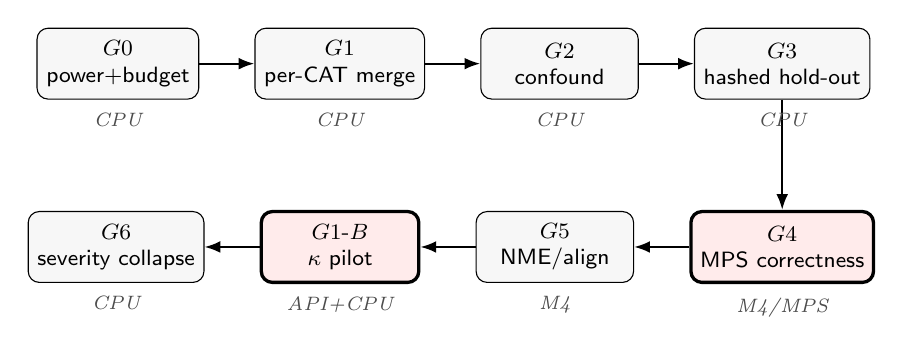
\begin{tikzpicture}[
  node distance=8mm and 7mm,
  gate/.style={draw, rounded corners, align=center, font=\footnotesize\sffamily,
               minimum height=9mm, minimum width=20mm, fill=gray!6},
  block/.style={draw, rounded corners, align=center, font=\footnotesize\sffamily,
               minimum height=9mm, minimum width=20mm, fill=red!8, very thick},
  flow/.style={-{Latex[length=2mm]}, thick},
  tag/.style={font=\scriptsize\itshape, gray!60!black}
]
\node[gate] (g0) {$G0$\\power+budget};
\node[gate, right=of g0] (g1) {$G1$\\per-CAT merge};
\node[gate, right=of g1] (g2) {$G2$\\confound};
\node[gate, right=of g2] (g3) {$G3$\\hashed hold-out};
\node[block, below=14mm of g3] (g4) {$G4$\\MPS correctness};
\node[gate, left=of g4] (g5) {$G5$\\NME/align};
\node[block, left=of g5] (g1b) {$G1\text{-}B$\\$\kappa$ pilot};
\node[gate, left=of g1b] (g6) {$G6$\\severity collapse};

\draw[flow] (g0) -- (g1);
\draw[flow] (g1) -- (g2);
\draw[flow] (g2) -- (g3);
\draw[flow] (g3) -- (g4);
\draw[flow] (g4) -- (g5);
\draw[flow] (g5) -- (g1b);
\draw[flow] (g1b) -- (g6);

\node[tag, below=0.5mm of g0] {CPU};
\node[tag, below=0.5mm of g1] {CPU};
\node[tag, below=0.5mm of g2] {CPU};
\node[tag, below=0.5mm of g3] {CPU};
\node[tag, below=0.5mm of g4] {M4/MPS};
\node[tag, below=0.5mm of g5] {M4};
\node[tag, below=0.5mm of g1b] {API+CPU};
\node[tag, below=0.5mm of g6] {CPU};
\end{tikzpicture}
\caption{Blocking gate dependency DAG. Arrows are hard predecessor constraints: a gate may not
run until its predecessor has written \texttt{PASS}. Bold nodes ($G4$, $G1\text{-}B$) are the
two gates that can block or pivot the entire spine --- $G4$ on silent compute-correctness,
$G1\text{-}B$ on the veterinary $\kappa$ pilot. Italic tags are the compute tier. $G1\text{-}B$
follows $G5$ because it needs aligned crops.}
\label{fig:gate-dag}
\end{figure}

\begin{table}[t]
\centering
\caption{Gate-by-gate exit artifact, blocking condition, and compute. Each gate writes
\texttt{artifacts/gateN/PASS}. ``Pivot'' rows can redirect the spine to the binary-plus-abstention
spine without killing the project; ``Blocking'' rows must turn green before any downstream number is
believed.}
\label{tab:gate-matrix}
\footnotesize
\begin{tabular}{@{}p{0.10\linewidth}p{0.40\linewidth}p{0.10\linewidth}p{0.30\linewidth}@{}}
\toprule
\textbf{Gate} & \textbf{Exit artifact + blocking condition} & \textbf{Compute} & \textbf{Kill / pivot} \\
\midrule
$G0$ & Committed single-integer vet budget + $\kappa$ floors + $\rho$-band decision in
\texttt{prereg.yaml}; three zero-data power calcs ($\kappa$ CI half-width $\leq 0.15$;
LTT/MAPIE NPV$\geq 0.90$ at $\leq 40\%$ abstention; $0.39$ CI reportability) &
CPU ($\tfrac{1}{2}$ day) &
If the NPV calc fails, abstention is exploratory-only (no ``guaranteed''); not a kill \\
\addlinespace
$G1$ & \texttt{folds.csv}; assert no individual straddles a fold; distinct-pain-cat
denominator printed and stored &
CPU &
Fall back to per-clip grouping with re-ID flagged as a limitation \\
\addlinespace
$G2$ & Confound result logged as ``no confound \emph{detected at this power}''; FGS-BG-Gap +
per-AU EBPG computed (one-directional) &
CPU, no vet &
Portable protocol $\Rightarrow$ proceed/co-headline; non-portable $\Rightarrow$
threat-to-validity \\
\addlinespace
$G3$ & Hashed cat-disjoint test manifest (\texttt{test\_ids.sha256}) + CI guard that aborts
any leaking run, demonstrated on a deliberate violation &
CPU &
Hard blocker: no scoring until the guard provably aborts a leak \\
\addlinespace
$G4$ & (a) MPS--CPU DINOv2 logit parity $\max|\Delta|<10^{-3}$; (b) 1-epoch CORN smoke test;
(c) synthetic decode$\to$sum$\to 0.39$ unit test &
M4/MPS &
\textbf{Blocking} --- no number believed until all three pass \\
\addlinespace
$G5$ & CatFLW-landmark NME inside crop vs eye-aligned crop + median face resolution, both
clearing \texttt{prereg.yaml} thresholds &
M4 &
\textbf{Blocking} for Phase~B; else add 2-point eye-similarity alignment and re-measure \\
\addlinespace
$G1\text{-}B$ & $\approx 120$-image ($\geq 50$ positive) per-AU quadratic $\kappa$ with CI;
GO iff orbital/ear/head $\kappa$\textbf{-LB} $\geq 0.60$ (muzzle/whiskers $0.40\text{--}0.60$
caveat) &
API + CPU &
$\kappa$-LB below floor $\Rightarrow$ \textbf{pivot to binary spine} (drop graded); not a kill \\
\addlinespace
$G6$ & Count vet-confirmed AU$=2$ cells; if any single-digit, collapse the high end
(pre-committed structural decision) &
CPU &
Expected to fire $\Rightarrow$ collapse; do \emph{not} print a per-cell severe number \\
\bottomrule
\end{tabular}
\end{table}

\paragraph{Cross-cutting kill triggers.} Two triggers cut across the gate order. First, the
Monte-Carlo robustness check of the cross-AU error correlation is run under both $\rho=0$ and a
pinned $\rho=0.3$; a GO under $\rho=0$ that becomes a NO-GO under $\rho=0.3$ declares the gate
\emph{fragile}, which is reported as such, and the build defaults to the binary-plus-abstention spine rather
than claim a GO that the correlation assumption could flip. Second, $G4$ or $G5$ failing is
absolutely blocking: no metric computed downstream of a silently-wrong MPS logit or a
misaligned crop is believed, because in that regime ``calibration'' would measure crop quality
rather than pain.

\paragraph{The modal product.} The gate system is designed so that the most probable outcome is
not a failure but a well-characterised \emph{binary-plus-wrapper} instrument:
binary pain decision $+$ the $\kappa$-as-method protocol (result pending the independent vet anchor) $+$ the confound-attribution protocol
$+$ the welfare decision curve $+$ the lower-bound abstention curve, with graded-CORN shipped as
an inspected-not-validated artifact. Every gate either advances this product or pivots cleanly
onto it.

\section{Reproducibility contract}
\label{sec:repro}

Reproducibility is treated as a gate property, not an afterthought: every gate inherits the
contract below, and two of its clauses are themselves blocking ($G3$ and $G4$).

\begin{itemize}
  \item \textbf{Single seed.} A single \texttt{seed\_everything(42)} seeds Python, NumPy,
        Torch, and MPS; no script re-seeds ad hoc.
  \item \textbf{Deterministic mode.} \texttt{torch.use\_deterministic\_algorithms(True,
        warn\_only=True)}, \texttt{PYTHONHASHSEED=42}, and \texttt{num\_workers=0} on the small
        corpus.
  \item \textbf{Provenance on every run.} The \texttt{git\_sha} and the Roboflow dataset
        version are injected into the experiment-tracker config and tags for every run, so any
        artifact is traceable to exact code and exact data.
  \item \textbf{Locked environment.} \texttt{uv.lock} and \texttt{.python-version} are
        committed; all runs go through \texttt{uv run} against the macOS MPS-capable wheels (no
        CUDA extras on the M4).
  \item \textbf{Frozen hashed test manifest (blocking, $G3$).} A CI test aborts any
        train/sweep that can read \texttt{test\_ids.sha256}.
  \item \textbf{Blocking Gate-4 unit tests.} The CORN decode$\to$sum$\to 0.39$ test and the
        MPS--CPU logit-parity test must pass in CI before any quantitative target runs; a red
        Gate~4 blocks Phase~B entirely.
  \item \textbf{Byte-frozen rubric cache.} The VLM rubric is byte-frozen and its hash pinned;
        any byte change invalidates the prompt cache, making accidental rubric drift
        detectable.
  \item \textbf{Firewall in code.} The sensitivity/specificity firewall (vet-only labels at
        $0.39$; $\kappa$ never used as validation) is enforced in the operating-point module,
        not merely described in prose.
\end{itemize}

The single deterministic-seed entry point is small enough to reproduce here:

\begin{verbatim}
def seed_everything(seed: int = 42):
    os.environ["PYTHONHASHSEED"] = str(seed)
    random.seed(seed); np.random.seed(seed); torch.manual_seed(seed)
    if torch.backends.mps.is_available(): torch.mps.manual_seed(seed)
    torch.use_deterministic_algorithms(True, warn_only=True)
\end{verbatim}

\section{Anti-benchmark reporting discipline}
\label{sec:anti-benchmark}

The instrument is framed as decision support, not as a leaderboard entry, and the reporting
discipline enforces that framing. The single hardest rule: \textbf{the document never claims to
``beat'' a prior accuracy figure} --- not the $77\%$ landmark or $65\%$ deep-learning binary
numbers, not the $79\%$, and not the $95.5\%$ automated-FGS pipeline number from the
literature. Such a comparison would be false rigor on a single-source corpus with a different
label semantics, a different prevalence, and a different evaluation unit. Prior published
numbers appear only as \emph{prior-art context} (for example, sourcing the fixed pain-recall
target from Evangelista's validated operating point), explicitly attributed and never staged as
a head-to-head win.

Concretely, the discipline requires that:

\begin{enumerate}
  \item Every rate is printed with its \textbf{distinct-pain-cat denominator} and a
        Clopper--Pearson or bootstrap interval; a bare percentage is never reported.
  \item \textbf{Augmented copies never enter any reported $N$}.
  \item The graded $0\text{--}10$ sum and its VLM-vs-vet $\kappa$ are labelled
        \textbf{internal / inspection-only}; the word ``graded'' is struck from every
        validated-claim sentence, and the abstract holds with the graded layer dropped.
  \item The confound result is phrased ``no confound \textbf{detected at this power},'' never
        ``no confound,'' reflecting that the audit is well-powered to detect entanglement and
        underpowered to rule it out.
  \item The output is always presented as triage --- ``grimace consistent with pain, $X/10$;
        recommend veterinary assessment'' --- and \textbf{never} as an autonomous analgesia
        trigger; the negative class is documented as an unknown mixture (possibly sedated or
        post-operative).
  \item The DINOv2$+$CORN engine is stated to be \textbf{conceded plumbing, not a novel
        contribution}; the claimed contributions are the two portable methods and the
        welfare-asymmetric wrapper.
\end{enumerate}

Taken together, the cross-validation design, the blocking gate order, the reproducibility
contract, and the anti-benchmark rules form a single evaluation contract whose purpose is to
make the eventual results \emph{believable in proportion to what the data can actually
support} --- and to make any overclaim structurally impossible to ship.

% !TeX root = ../main.tex
% Chapter 7 -- Expected Outcomes, Gate-Conditioned Decisions, and Risk Analysis
% Self-contained section file: no preamble, no \documentclass.
% HONESTY RULE: no experiments have been run. This chapter replaces a "Results"
% chapter with an EXPECTED / GATE-CONDITIONED OUTCOMES framing. Every quantitative
% figure that appears as a number belongs to the LITERATURE and is attributed as such.
%
% PREAMBLE REQUIREMENTS (main.tex must load these):
%   \usepackage{booktabs}
%   \usepackage{tikz}
%   \usetikzlibrary{arrows.meta,positioning}
% The TikZ gate tree uses arrows.meta (Latex tips) and positioning (below=of / right=of).

\chapter{Expected Outcomes, Gate-Conditioned Decisions, and Risk Analysis}
\label{ch:expected-outcomes}

\newcommand{\evangelistanums}{AUC~$0.94$ / sensitivity~$90.7\%$ / specificity~$86.6\%$}

\begin{quote}\small\itshape
No experiments have been run, and the no-results stance is structural rather than a
stylistic choice: the corpus has not been forked (the repository's \texttt{data/}
substrate is empty), no independent per-AU veterinary anchor exists, and the only
available source is a Roboflow \emph{binary} pain corpus with no native $0$--$10$ FGS
labels. This chapter therefore contains no measured results, no accuracies, no
$\kappa$ values, no calibration numbers, and no figures of our own curves. It states,
per gate, the \emph{decision rule} and the gate-conditioned outcome
(\textsc{go} / \textsc{pivot} / \textsc{collapse}), the modal product we plan to ship,
and the kill criteria under which we pivot. Every numeric value that appears
(e.g. \evangelistanums) is drawn from the prior literature and is explicitly
attributed to its authors as a \emph{background anchor}, never as a result of this
work. Real-cat evaluation is named throughout as future work; the present
contribution is a methods/protocol specification.
\end{quote}

This chapter deliberately departs from the template's Chapter~4
(\emph{การทดลองและผลลัพธ์}, Experiments and Results). Because the project is a
research proposal and methodology with a strict, artifact-emitting gate order
rather than a completed empirical study, a conventional results chapter would
either be empty or be forced to fabricate numbers. We therefore recast the
chapter as an \emph{expected-outcomes and risk} analysis: for each gate we
pre-register the decision rule, the pass/fail branch, and exactly what ships in
each case. The chapter is organised around the \emph{modal deliverable}
(\S\ref{sec:modal-deliverable}), the gate-conditioned decision table
(\S\ref{sec:decision-table}), the power-calculation-conditioned framing of the
abstention curve (\S\ref{sec:power-conditioned}), the expected severity-cell
collapse (\S\ref{sec:severity-collapse}), the Monte-Carlo correlation-sensitivity
band (\S\ref{sec:rho-band}), and the literature anchors we cite as background
(\S\ref{sec:lit-anchors}).

%====================================================================
\section{The Modal Deliverable as the Default Product}
\label{sec:modal-deliverable}

We plan the repository, the evaluation protocol, and the write-up for the
\emph{modal} outcome --- the product we expect to ship --- not the optimistic one.
The modal deliverable is a \textbf{binary-pain decision-support instrument with a
trustworthiness wrapper}, headlined by a power-conditioned, per-AU
confound-attribution protocol and accompanied by a guarded VLM-as-AU-rater $\kappa$
reliability check, shipped on an explicitly-conceded engine. The graded $0$--$10$ Feline Grimace Scale (FGS) layer
is present strictly as an \emph{inspected-not-validated} artifact. The single
governing rule on the prose: \textbf{the abstract must hold with the graded layer
dropped}, and the word ``graded'' is struck from every validated-claim sentence.

Concretely, the modal product comprises six named components, summarised in
Table~\ref{tab:modal-components}. Four are validated claims (Components~1--4);
Component~5 (the NPV/abstention curve) is reported only as placeholder-illustrative
sizing, never as a validated number; and the sixth (the graded CORN layer) is never
entered into a validated results table.

\begin{table}[t]
\centering
\caption[The six components of the modal deliverable]{The six components of the
modal deliverable. The abstract is required to hold with Component~6 dropped; the
DINOv2+CORN engine is conceded as plumbing and is never claimed novel. ``Validated''
means estimated against vet-confirmed labels under the circularity firewall.}
\label{tab:modal-components}
\small
\begin{tabular}{@{}clp{0.40\linewidth}c@{}}
\toprule
\# & Component & What it is & Validated? \\
\midrule
1 & Calibrated binary decision &
  Per-image pain decision at a \emph{fixed pain-recall} $\geq 0.90$ operating
  point (after \citealp{evangelista2019}); never Youden-$J$/$F_1$ & Yes \\
2 & Confound-attribution protocol &
  FGS-BG-Gap (background-swap primitive \citep{xiao2021noise,moayeri2022comprehensive})
  $+$ per-AU EBPG (Score-CAM energy-based pointing-game primitive
  \citep{wang2020scorecam}; distinct from the per-AU saliency-alignment framing of
  \citet{lencioni2025segment}), \emph{one-directional} (``no confound detected at
  this power'' \citep{adebayo2022posthoc}) & Yes (headline) \\
3 & $\kappa$ reliability check &
  Per-AU VLM-vs-vet quadratic-weighted $\kappa$ \citep{cohen1968kappa} reported on
  its \emph{CI lower bound} --- a standard clinimetric acceptance gate
  \citep{tractenberg2010kappa,donner2010kappa,rotondi2012kappa,rotondi2018kappasize,simwright2005kappa},
  not novel here; guarded, inspected-not-validated & Yes (guarded check) \\
4 & Welfare-asymmetric decision curve &
  Net-benefit decision-curve analysis \citep{vickers2006dca} with the
  undertreat:overtreat harm ratio swept as a \emph{range} & Yes \\
5 & LB-abstention curve &
  One-sided $95\%$ NPV \emph{lower bound} at each abstention rate
  \citep{angelopoulos2021ltt}; ``guaranteed'' is banned & Illustrative (placeholder sizing) \\
6 & Inspected graded-CORN &
  $5$ per-AU CORN heads \citep{shi2023corn} $\to$ $0$--$10$ sum $\to$ pmf;
  inspected-not-validated & \textbf{No} \\
\bottomrule
\end{tabular}
\end{table}

The headline contribution is Component~2 (the power-conditioned, per-AU
confound-attribution protocol); Component~3 (the VLM-as-AU-rater $\kappa$) is a
guarded reliability check held below it as kill-tree insurance, not a co-equal
second pillar. Both ship as released, runnable, dataset-agnostic code. Novelty is
claimed for the \emph{assembly} and the per-AU EBPG-as-confound-evidence
instantiation of equivalence-style audit hygiene, never for any individual primitive
or the one-directional / power-conditioned statistics themselves
\citep{huanghooker2026fairness,singh2023samplesize}. The calibration, RPS,
ClasswiseECE, and conformal machinery are \emph{cited supporting evidence}, never
headlines. The engine (frozen DINOv2 ViT-S/14 --- with the \texttt{\_reg}
register variant (\texttt{dinov2\_vits14\_reg}) the field default, A/B'd before
locking ViT-S/14 because registers suppress attention artifacts that hurt the
dense, localized per-AU features
\citep{oquab2023dinov2} feeding the CORN ordinal heads \citep{shi2023corn}) is
conceded as plumbing and is never presented as novel.

%====================================================================
\section{The Gate-Conditioned Decision Table}
\label{sec:decision-table}

The project executes a strict, blocking gate order: \textbf{G0}
(power calcs and vet-budget pre-registration) $\to$ \textbf{G1} (per-CAT merge)
$\to$ \textbf{G2} (capture-condition confound audit) $\to$ \textbf{G3} (frozen
hashed cat-disjoint hold-out) $\to$ \textbf{G4} (MPS compute-correctness, blocking)
$\to$ \textbf{G5} (alignment/NME) $\to$ \textbf{G1-B} (weak-label reliability
$\kappa$ pilot) $\to$ \textbf{G6} (severity-cell collapse). Each gate carries a
\emph{pre-registered} decision rule; passing a gate is a precondition for the work
downstream of it, and failing a gate routes to a pre-committed branch rather than
to an improvised fix. Figure~\ref{fig:gate-tree} renders the gate order as a
decision tree terminating in the modal product, and Table~\ref{tab:kill-crosswalk}
gives the kill/pivot crosswalk in full.

\begin{figure}[t]
\centering
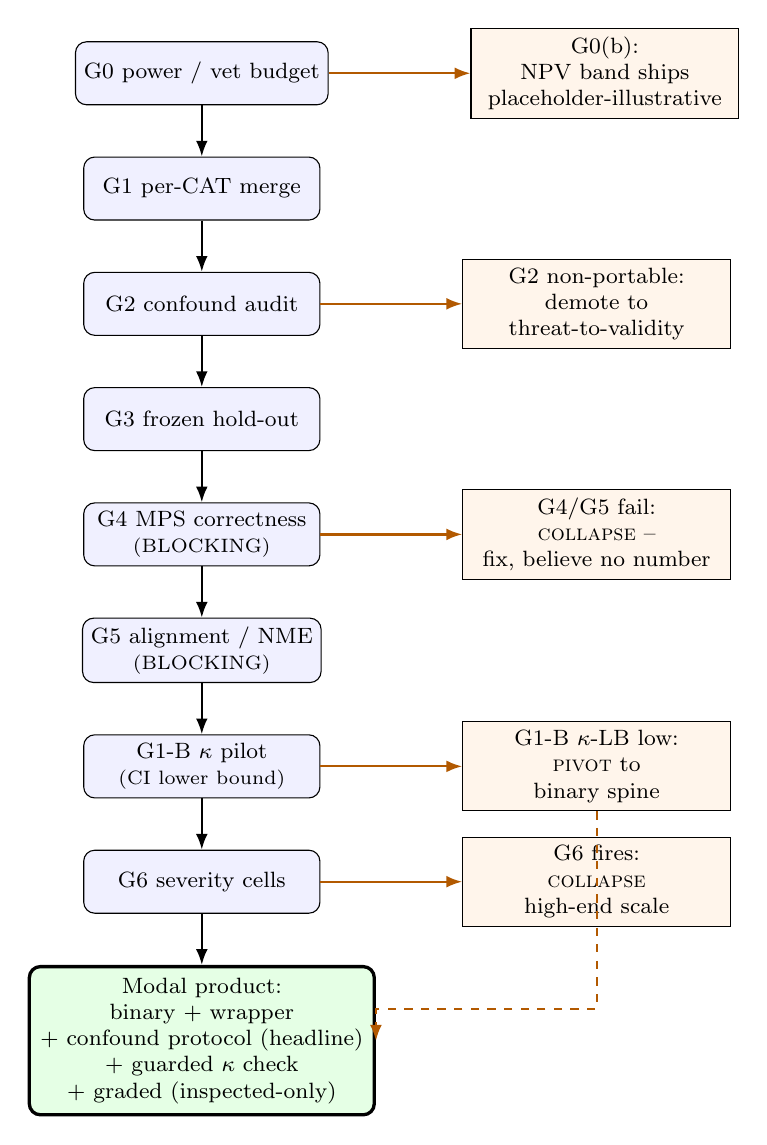
\begin{tikzpicture}[
  node distance=6.5mm and 9mm,
  every node/.style={font=\footnotesize},
  gate/.style={rectangle, rounded corners, draw, fill=blue!6, align=center,
               minimum width=30mm, minimum height=8mm, inner sep=3pt},
  branch/.style={rectangle, draw, fill=orange!8, align=center,
                 minimum width=34mm, inner sep=3pt},
  ship/.style={rectangle, rounded corners, draw, very thick, fill=green!10,
               align=center, minimum width=42mm, inner sep=4pt},
  flow/.style={-{Latex[length=2mm]}, thick},
  sidelab/.style={font=\scriptsize\itshape}
]
% main spine
\node[gate] (g0) {G0 power / vet budget};
\node[gate, below=of g0] (g1) {G1 per-CAT merge};
\node[gate, below=of g1] (g2) {G2 confound audit};
\node[gate, below=of g2] (g3) {G3 frozen hold-out};
\node[gate, below=of g3] (g4) {G4 MPS correctness\\\scriptsize(BLOCKING)};
\node[gate, below=of g4] (g5) {G5 alignment / NME\\\scriptsize(BLOCKING)};
\node[gate, below=of g5] (g1b) {G1-B $\kappa$ pilot\\\scriptsize(CI lower bound)};
\node[gate, below=of g1b] (g6) {G6 severity cells};
\node[ship, below=of g6] (modal) {Modal product:\\binary $+$ wrapper\\$+$ confound protocol (headline)\\$+$ guarded $\kappa$ check\\$+$ graded (inspected-only)};

\foreach \a/\b in {g0/g1, g1/g2, g2/g3, g3/g4, g4/g5, g5/g1b, g1b/g6, g6/modal}
  \draw[flow] (\a) -- (\b);

% branch outcomes on the right
\node[branch, right=18mm of g0] (g0b) {G0(b):\\NPV band ships\\placeholder-illustrative};
\node[branch, right=18mm of g2] (g2b) {G2 non-portable:\\demote to\\threat-to-validity};
\node[branch, right=18mm of g4] (g4b) {G4/G5 fail:\\\textsc{collapse} --\\fix, believe no number};
\node[branch, right=18mm of g1b] (g1bb) {G1-B $\kappa$-LB low:\\\textsc{pivot} to\\binary spine};
\node[branch, right=18mm of g6] (g6b) {G6 fires:\\\textsc{collapse}\\high-end scale};

\draw[flow, orange!70!black] (g0) -- (g0b);
\draw[flow, orange!70!black] (g2) -- (g2b);
\draw[flow, orange!70!black] (g4) -- (g4b);
\draw[flow, orange!70!black] (g1b) -- (g1bb);
\draw[flow, orange!70!black] (g6) -- (g6b);

% pivots still terminate in a publishable product
\draw[flow, dashed, orange!70!black] (g1bb.south) |- ([yshift=4mm]modal.east) -- (modal.east);
\end{tikzpicture}
\caption[Gate-conditioned decision tree]{Gate-conditioned decision tree. The left
spine is the \textsc{go} path through gates G0$\to$G6 terminating in the modal
product. The right column shows the pre-registered branch at each gate. Note that
no branch is a project-killing null: a G1-B \textsc{pivot} drops the graded layer
but still ships the calibrated binary spine, the headline confound protocol, and
the guarded $\kappa$ check (dashed arrow). G4/G5 are blocking correctness gates --- a
failure halts reporting until fixed, never silently degrades a number.}
\label{fig:gate-tree}
\end{figure}

\begin{table}[t]
\centering
\caption[Kill/pivot crosswalk]{Kill/pivot crosswalk (gate $\to$ branch $\to$ what
ships), after the kill criteria of the finalised direction. Every branch remains
publishable; the only ``hard stop'' branches are the blocking correctness gates
G4/G5, which halt reporting until the defect is fixed rather than ending the
project.}
\label{tab:kill-crosswalk}
\footnotesize
\begin{tabular}{@{}p{0.13\linewidth}p{0.36\linewidth}p{0.42\linewidth}@{}}
\toprule
Gate & Failing branch (trigger) & What ships on that branch \\
\midrule
G0(b) &
  NPV sizing rests on a placeholder budget over zero data (not yet certifiable) &
  \textsc{proceed}; the abstention curve (Component~5) is reported as
  \emph{placeholder-illustrative} with a one-sided $95\%$ lower bound;
  ``guaranteed'' never appears. Not a kill --- relocates the deliverable onto the
  welfare decision curve. \\[2pt]
G2 &
  Audit damning but yields only ``CAT\_01 is confounded'' (non-portable) &
  Demote the audit to a threat-to-validity paragraph; the guarded $\kappa$ check
  becomes the sole-survivor headline (kill-tree insurance). If G1-B \emph{also}
  fails, the honest paper is a confound/audit note (venue pre-registered now). \\[2pt]
G2 &
  Confounding detected as a \emph{transportable protocol} &
  \textsc{proceed} --- this is the headline leg, publishable even if everything
  downstream is null \citep{xiao2021noise,moayeri2022comprehensive}. \\[2pt]
G1-B &
  $\kappa$ CI lower bound below floor on orbital/ear/head &
  \textsc{pivot} to binary spine: \emph{drop graded entirely}; ship calibrated
  binary $+$ abstention $+$ the headline confound protocol. The guarded $\kappa$
  check and the cited wrapper still stand (the $\kappa$ protocol remains runnable,
  with its result pending the independent vet anchor). \\[2pt]
G1-B &
  Passes orbital/ear/head; fails muzzle/whiskers &
  \textsc{proceed} on the surviving AUs; state how dropping $2$ of $5$ heads
  shifts the achievable $0$--$10$ range and whether $0.39$ ($\approx 4/10$) is
  even reachable. \\[2pt]
G4 / G5 &
  MPS logit parity / decode unit test / NME audit fails &
  \textsc{blocking}: fix before any metric is believed. No number from
  silently-wrong logits or misaligned crops is reported. \\[2pt]
G6 &
  AU=2 (severe) cells single-digit &
  \textsc{collapse} the high-end scale (pre-committed); do \emph{not} print a
  per-cell severe calibration number. Expected to fire (see
  \S\ref{sec:severity-collapse}). \\[2pt]
$\rho$-band &
  Monte-Carlo \textsc{go} under $\rho=0$ but \textsc{no-go} under $\rho=0.3$ &
  Declare the gate \emph{fragile}; default to the binary fallback rather than
  claim a \textsc{go} the correlation could flip (\S\ref{sec:rho-band}). \\
\bottomrule
\end{tabular}
\end{table}

The structural property we want from Table~\ref{tab:kill-crosswalk} is that
\emph{no branch is a project-killing null}. The headline confound-attribution
protocol is designed to be independently publishable: a confounding signal detected
as a transportable, power-conditioned protocol stands regardless of downstream
outcomes. Below it, the guarded per-AU $\kappa$ check is a runnable protocol for
measuring whether a frozen vision-language model can weak-label feline FGS action
units at human-rater agreement (the result is pending an independent per-AU vet
anchor, and is only a weak-labeling-capability measurement if that anchor is
independent and the VLM's rubric differs from the vet's --- otherwise it measures
rubric-following); it is retained as kill-tree insurance, becoming the
sole-survivor headline only if the confound leg degrades. The binary-plus-wrapper
spine is the floor that stands today --- the likely v1 ship --- with the graded
layer as upside conditional on the Gate-1-B $\kappa$ pilot passing.

%====================================================================
\section{Power-Calculation-Conditioned Framing of Abstention}
\label{sec:power-conditioned}

The abstention curve (Component~5) is the component most exposed to the project's
single binding constraint: every quantitative claim ultimately draws on the same
modest vet-confirmed anchor (a Gate-0 placeholder of $120$ confirmed images,
$\geq 50$ pain-positive, echoed from \texttt{configs/power.yaml} and to be replaced
before any quantitative claim; this integer is an unconfirmed placeholder over
zero data, not a power-backed figure). Gate~0 runs three zero-data power
calculations: (a) the number of faces needed for a per-AU $\kappa$ CI half-width
$\leq 0.15$ (the committed budget meets this floor); (b) the number needed for a
Learn-Then-Test / conformal NPV $\geq 0.90$ at an abstention rate $\leq 40\%$
\citep{angelopoulos2021ltt}; and (c) whether the $0.39$-threshold operating-point
CI is reportable at the budgeted $n$.

\textbf{The committed Gate-0 verdict on (c) is negative.} At the budgeted anchor the
$0.39$ per-class sensitivity/specificity operating point rests on only $n_{\text{pos}}
= 16$ positives, giving a Clopper--Pearson half-width of $\approx 0.25$; the power
calculation accordingly flags it \texttt{reportable:false}. We therefore do
\emph{not} treat the $0.39$ point as a result of this work: it is carried as an
exploratory, future-work quantity and named as a limitation, not as an open question
to be settled at the present budget.

The Gate-0(b) NPV sizing is, at the present budget, a \emph{placeholder-illustrative}
calculation, not a settled certification. Its inputs are exploratory --- a
placeholder \texttt{vet\_budget} of $120$, a worked total of $84$ faces, and a
target NPV of $0.90$ over zero measured data --- so although the calculation marks
the band as nominally meeting the target, we do \emph{not} report that band as
``certified'' or ``guaranteed.'' The band is not yet certified because the budget is
an unconfirmed placeholder over an empty corpus, not because any arithmetic forbids
it; whether a real, non-placeholder budget can certify a useful NPV floor on
measured data is future work. The decision rule we pre-register is one of
\emph{reporting discipline}: the word ``guaranteed'' never appears anywhere in the
paper, and the abstention curve is reported only as ``NPV with a one-sided $95\%$
lower bound at each abstention rate'' --- a finite-sample statement. The $0.95$
arithmetic is retained for one purpose only: to make the ban concrete. Certifying
NPV~$\geq 0.95$ would, at this scale, demand on the order of $60$ zero-error
abstained-in negatives out of ${\sim}70$ total, which is exactly the kind of
fragile, near-vacuous claim a point ``guarantee'' would smuggle in --- hence the
one-sided lower bound and the placeholder framing rather than a deliverable
certificate. Should the placeholder sizing not survive a real budget, the headline
weight of the wrapper relocates onto the welfare-asymmetric decision curve
(Component~4), the more robust artifact at small $n$; this is a relocation, not a
kill.

%====================================================================
\section{Expected Severity-Cell Collapse (Gate 6)}
\label{sec:severity-collapse}

Gate~6 is a pure-counting gate applied after the vet anchor exists: it counts the
number of vet-confirmed AU=2 (severe) cells per action unit. The pre-registered
rule is that if any AU's $=2$ cell count is single-digit, the high end of the
scale is \emph{collapsed} (merge the $1$ and $2$ levels, or report only
painful/not-above-threshold). This is a structural decision, not a caveat: a
caveat would leave an anchoring number in a table, whereas an AU=2 sensitivity
estimate at single-digit $n$ carries a confidence interval spanning roughly
$[0.35, 0.97]$ --- that is no information.

\textbf{We expect Gate~6 to fire.} Given the ${\sim}12$--$13\%$ pain prevalence of
the source corpus and the further rarity of \emph{severe} grimace within the pain
class, the budgeted anchor is very unlikely to deliver double-digit AU=2 cells.
Planning for the collapse in advance --- rather than treating it as a surprise ---
is what keeps the graded layer honest: no per-cell severe calibration number is
printed, and the graded layer remains an inspected-not-validated artifact. This is
the operational reason the word ``graded'' is struck from every validated-claim
sentence; the low-prevalence measurement-error dynamics that make such tail cells
untrustworthy are exactly those characterised by \citet{chavoshi2025}, whose
analysis shows how a high apparent agreement can coexist with a badly degraded
operating sensitivity once prevalence is low.

%====================================================================
\section{Monte-Carlo Correlation-Sensitivity Band}
\label{sec:rho-band}

A naive plan would estimate a full $5\times5$ cross-AU error-correlation matrix
from the anchor and feed it into the error-propagation Monte-Carlo. At the
budgeted $n$ this is false rigor: a ten-off-diagonal matrix has per-entry
confidence intervals on the order of $[-0.4, +0.6]$, may not even be
positive-definite, and launders sampling noise as data-driven structure. We
therefore replace it with a \textbf{two-point $\rho$-sensitivity band}: the
error-propagation Monte-Carlo is run twice, once under independence ($\rho = 0$)
and once under a pinned uniform correlation ($\rho = 0.3$), and the gate returns
\textsc{go} \emph{only if the decision holds under both}.

The decision rule is pre-registered (Table~\ref{tab:kill-crosswalk}, final row):
if the Monte-Carlo is \textsc{go} under $\rho = 0$ but \textsc{no-go} under
$\rho = 0.3$, we declare the gate \emph{fragile}, say so explicitly, and default to
the binary fallback rather than claim a \textsc{go} that a plausible correlation
could flip. A pinned $\rho$ is an honest sensitivity analysis; a noisily-fit
matrix would be a false claim of empirical precision. The two-point band is the
conservative substitute that we can defend at this sample size; the full matrix is
explicitly deferred (re-added only when $n$ reaches the low hundreds of vet rows
with non-single-digit cells).

%====================================================================
\section{Literature Anchors as Background, Never as Our Results}
\label{sec:lit-anchors}

The numbers in Table~\ref{tab:lit-anchors} are the prior literature's, cited as
\emph{background anchors} that motivate our design choices --- chiefly the
fixed-recall operating point and the anti-benchmark reporting discipline. \textbf{None
of these figures is a result of this work}, and the paper never makes a
``we beat $77/79/95\%$'' claim. We report against the distinct-pain-cat
denominator with Clopper--Pearson / bootstrap confidence intervals, and the
literature figures appear only as prior-art context, never as a head-to-head
comparison.

\begin{table}[t]
\centering
\caption[Literature background anchors]{Literature background anchors. Every figure
below belongs to the cited authors and is reproduced here as background context for
our design --- \emph{not} as a result of this work. We do not benchmark against
these numbers; they motivate the fixed pain-recall $\geq 0.90$ operating point and
the decision-support framing.}
\label{tab:lit-anchors}
\footnotesize
\begin{tabular}{@{}p{0.20\linewidth}p{0.34\linewidth}p{0.36\linewidth}@{}}
\toprule
Source (theirs) & Their reported figure & How we use it (background only) \\
\midrule
\citet{evangelista2019} &
  FGS validation: \evangelistanums{}; pain at a $>0.39$ ($\approx 4/10$) threshold &
  Sources our fixed pain-recall $\geq 0.90$ \emph{target} and the $0.39$ decision
  cutoff; never a comparison baseline. \\[2pt]
\citet{steagall2023} &
  Automated FGS via landmark$\to$geometry$\to$XGBoost, $95.5\%$ accuracy &
  Names a method family (landmark$+$XGBoost) we deliberately do \emph{not}
  replicate; cited to position our conceded-engine choice. \\[2pt]
\citet{feighelstein2023} &
  Binary cat-pain: landmark $77\%$ vs.\ deep-learning $65\%$; XAI mouth $>$ eyes
  $>$ ears &
  Background for the binary spine and for AU saliency expectations; not a target
  to beat. \\[2pt]
\citet{chavoshi2025} &
  Low-prevalence measurement-error propagation (e.g.\ ${\sim}10\%$ prevalence
  $\to$ ${\sim}53\%$ effective sensitivity) &
  Motivates the severity-cell collapse (\S\ref{sec:severity-collapse}) and the
  low-prevalence CI discipline. \\
\bottomrule
\end{tabular}
\end{table}

\paragraph{Restatement of the honesty contract.}
To close the chapter, we restate its governing constraint without hedging.
\emph{No experiments have been run.} This chapter contains no measured results.
The gate-conditioned outcomes above are pre-registered decision rules and the
products that ship on each branch, not observations. The only numbers presented
are the literature anchors of Table~\ref{tab:lit-anchors}, each attributed to its
authors. When the project executes, every reported figure will carry its
distinct-pain-cat denominator and a Clopper--Pearson or bootstrap confidence
interval, sensitivity and specificity at the $0.39$ cutoff --- a quantity the
Gate-0 power calc flags \texttt{reportable:false} at the budgeted
$n_{\text{pos}} = 16$, hence exploratory pending a future enlarged vet anchor ---
will be estimated on vet-confirmed labels only (the circularity firewall), and the
agreement between the model and the weak-labeling VLM will never be presented as
validation. The
modal product --- the binary-plus-wrapper instrument headlined by the
confound-attribution protocol, with the guarded $\kappa$ check below it and an
inspected-not-validated graded layer --- is the outcome we plan for, and it
stands even if the graded layer is dropped entirely.

% Chapter 8 -- Ethics, Welfare Framing, and Limitations
% Self-contained section file: no preamble, no \documentclass.
% Mirrors the template's Chapter 5, Sec. 5.3 (Limitations, itemized, each tied to a concrete cause),
% expanded to the project's welfare/ethics stance.
% HONESTY RULE: this is a methodology / research-proposal chapter. No experiments have been run
% and no result numbers of ours are reported. Literature anchors are attributed as background.

\chapter{Ethics, Welfare Framing, and Limitations}
\label{ch:ethics-welfare-limitations}

This chapter states the ethical and welfare commitments that govern how the
instrument may be used, and then enumerates --- candidly, in the itemized style
of the template's limitations section --- the constraints that bound every claim
this work makes. It is written in the same self-honesty register as the rest of
the document: because no experiments have yet been conducted, the chapter
reports no outcomes of our own. What it fixes instead is the framing under which
any future outcome would be permitted to circulate, the measurement-error
consequences we already know our data will impose, and the descope triggers that
convert each limitation into a pre-committed decision rather than a post-hoc
excuse.

\section{Decision-Support Triage Framing Only}
\label{sec:triage-framing}

The instrument is a \emph{decision-support triage} tool and nothing more. Its
permitted output is a single sentence of the form \emph{``grimace consistent
with pain, $X/10$; recommend veterinary assessment''}, and the role of that
sentence is to surface a candidate for human attention, not to take any action
on the animal. The system is \textbf{never} an autonomous analgesia trigger:
under no configuration does a score, a threshold crossing, or an abstention
cause a drug to be administered, withheld, or dosed without a clinician in the
loop. This is a hard design boundary, not a deployment recommendation, and it is
restated in the released model card and datasheet so that a downstream
integrator cannot quietly repurpose the output as a control signal.

This framing follows directly from the welfare-asymmetric loss that motivates
the entire wrapper. The two error directions are not symmetric in their
consequences: a missed painful cat (a false negative) leaves an animal in
untreated pain, whereas a false alarm (a false positive) costs a clinician's
review and, at worst, an unnecessary examination. Because the harms are
asymmetric, the operating point is fixed at a high pain-recall target
($\geq 0.90$, anchored to the FGS validation level reported
by~\cite{evangelista2019}) rather than at a symmetric-cost Youden-J or $F_1$
knee, and the headline wrapper artifact is a harm-ratio-weighted decision curve
that sweeps the undertreat-to-overtreat asymmetry as a \emph{range} (we have no
vet-elicited point ratio, so we report the range and let the reader locate their
own loss on it). The triage framing is the ethical counterpart of that loss:
precisely because we tune the instrument to over-refer rather than under-refer,
the output must terminate at a recommendation for human assessment and may not
short-circuit into autonomous treatment. An instrument calibrated to flag
generously is safe only if a human adjudicates each flag.

\begin{figure}[t]
  \centering
  \fbox{\begin{minipage}{0.82\linewidth}
    \vspace{0.4em}
    \centering
    \textbf{[Captioned placeholder --- triage-output card mock]}\\[0.6em]
    \begin{flushleft}
    \small
    \texttt{------------------------------------------}\\
    \texttt{ FELINE PAIN TRIAGE (decision support)}\\
    \texttt{------------------------------------------}\\
    \texttt{ Grimace consistent with pain.}\\
    \texttt{ Estimated FGS-style score:  X / 10}\\
    \texttt{ Recommendation: REFER FOR}\\
    \texttt{   VETERINARY ASSESSMENT.}\\[0.4em]
    \texttt{ This is NOT a diagnosis and NOT an}\\
    \texttt{ analgesia trigger. A clinician must}\\
    \texttt{ adjudicate. [defer / abstain shown}\\
    \texttt{ when below NPV lower-bound floor]}\\
    \texttt{------------------------------------------}
    \end{flushleft}
    \vspace{0.2em}
  \end{minipage}}
  \caption[Triage-output card mock]{Captioned placeholder for the triage-output
  card the instrument is permitted to emit. The card surfaces a candidate for
  human review and explicitly disclaims diagnosis and autonomous analgesia. The
  $X/10$ figure is shown for inspection only; per Chapter~\ref{ch:ethics-welfare-limitations}
  the $0$--$10$ ordinal layer is inspected-not-validated and is never a validated
  claim. This is a design mock, not a screenshot of a built system.}
  \label{fig:triage-card}
\end{figure}

\section{Negative-Class Ambiguity and Low-Prevalence Measurement Error}
\label{sec:negative-class}

The corpus carries only binary \texttt{pain}/\texttt{no\_pain} boxes, and the
negative class is best understood as an \emph{unknown mixture}. The images
labelled \texttt{no\_pain} are not guaranteed to be cats in a clean baseline
state; the class plausibly contains sedated, post-operative, or
post-recovery animals whose facial expression is suppressed for reasons
unrelated to the absence of pain. We document this in the datasheet as a known
property of the labels rather than treating ``no pain'' as a clean physiological
ground truth. The pain labels themselves are, until the confound audit and the
weak-label kappa pilot pass, unvalidated pseudo-labels on a generic photo
corpus, and we treat them as such.

This ambiguity has a concrete statistical consequence that we do not get to wish
away, because it interacts with the corpus's low pain prevalence. At a
prevalence near $13\%$, even a label channel with seemingly modest error
propagates into a severely degraded effective sensitivity once the base rate is
folded in; the measurement-error analysis of~\cite{chavoshi2025} makes this
quantitative, showing how a low-prevalence regime can drive an apparently
acceptable instrument down to roughly half its nominal sensitivity once
label noise is accounted for. We therefore treat negative-class ambiguity not as
a footnote but as a first-order threat to every quantitative claim, and we
respond to it structurally: the sensitivity and specificity of the $0.39$
decision are estimated \emph{only} on vet-confirmed labels (the circularity
firewall), the prevalence is always reported on a fixed metadata basis with its
discrepancy logged, and every reported count carries its distinct-pain-cat
denominator together with Clopper--Pearson or bootstrap confidence intervals so
that the reader can see the finite-sample uncertainty rather than a bare point
estimate.

\section{Limitations}
\label{sec:limitations}

Mirroring the template's itemized limitations section, we enumerate the binding
constraints of this work, each tied to a concrete cause and, where one exists,
to a pre-committed mitigation or descope trigger. None of these is hidden in
prose elsewhere; they are collected here so a reader can audit the gap between
what the instrument could in principle claim and what its data and budget
actually license. Table~\ref{tab:limitations} summarizes the mapping from
limitation to cause to mitigation.

\paragraph{Single-source corpus and a lone camera identity.}
The entire spine is instantiated on one forked corpus, and the only known camera
identity in it is a single label (\texttt{CAT\_01}, the lone known camera id).
There is no second cohort, no second site, and no external validation set.
Consequently we make \textbf{no external-cohort or cross-site generalization
claim} of any kind: every reported number characterizes behaviour on this
corpus only, and the portability we do claim lives in the \emph{methods} ---
chiefly the headline confound-attribution protocol, supported by the guarded
VLM-as-AU-rater kappa reliability check --- which are released as runnable code
that the next corpus can re-run --- not in any number
this corpus produces.

\paragraph{The vet-anchor budget wall.}
Every quantitative claim that requires trustworthy graded labels --- the per-AU
kappa, the $0.39$ sensitivity/specificity, the abstention NPV lower bound, the
severity cells --- draws on the \emph{same} small veterinary anchor, on the
order of fifty pain-positive images, whose exact size is fixed by the Gate-0
power calculation. This single budget is the project's dominant constraint. At
this $n$ the severity tail is essentially unestimable, a ``guaranteed'' NPV is
arithmetically undeliverable, and a data-fitted cross-AU error-correlation
matrix would launder noise as rigor. We respond by budgeting the anchor up front
and by demoting any claim the budget cannot support \emph{on paper now} rather
than discovering its weakness later.

\paragraph{Synthetic-and-planted-control validation; no real-cat run yet.}
At the time of writing the released evidence is the protocol exercised on
\emph{synthetic data with planted positive and negative controls}
(\texttt{src/protocols/standalone\_test\_corpus.py}): the confound-attribution
protocol is validated by showing it fires on a deliberately planted confound and
stays silent on a deliberately clean control, not yet on real feline imagery. The
data directory (\texttt{data/}) ships empty, no per-AU veterinary anchor exists, the
corpus is Roboflow binary-only, and the $0.39$ operating point is currently a
\texttt{reportable:false} placeholder at $n_{\text{pos}}{=}16$ --- below the
pre-registered reportability floor. We therefore present this work as a
methods/protocol paper on synthetic and planted controls; \textbf{application to a
real-cat corpus is named explicitly as future work}, and no real-data number is
claimed here.

\paragraph{The graded layer is inspected-not-validated.}
The $0$--$10$ ordinal CORN layer is built, but it ships as an internally
consistent, VLM-anchored, qualitatively inspected exploratory artifact. The word
``graded'' is struck from every validated-claim sentence, and the abstract and
every results claim are written to hold with this layer dropped. There is no
independent per-AU $0/1/2$ gold held-out set on the solo timeline, so a validated
graded instrument is explicitly out of scope; the gold-set chase was cut from
the critical path precisely because the only candidate sets are either a category
error as a graded anchor (landmarks, not AU scores) or carry unbounded
request-only access dependencies.

\paragraph{Muzzle and whiskers kappa fragility.}
We expect the per-AU agreement to be strongest on the orbital, ear, and head
units and weakest on the muzzle and whiskers, in line with the relative
difficulty of those units reported in prior feline-pain
work~\cite{feighelstein2023}. The Gate-1-B floors reflect this asymmetry
(higher floor for orbital/ear/head, a lower acceptable-with-caveat band for
muzzle/whiskers), and the gate fires on the confidence-interval \emph{lower
bound} rather than the point estimate. If the orbital/ear/head floor is not
cleared, the graded layer is dropped entirely and the project pivots to the
calibrated binary-plus-abstention spine; if only muzzle/whiskers fail, we
proceed on the surviving units and state how dropping two of five heads narrows
the achievable $0$--$10$ range.

\paragraph{CatFLW licensing blocks commercial deployment.}
The landmark set used for the alignment and NME audit, CatFLW, is licensed
CC~BY-NC~4.0~\cite{martvel2024catflw}; it is non-commercial, the aligner trained
on it inherits that restriction, and it therefore blocks any commercial
deployment of a derived model. We keep it strictly walled from the CC~BY corpus
so a derived release stays CC~BY, and we use CatFLW for alignment and NME only,
never as a graded anchor.

\paragraph{The confound audit is one-directional.}
The capture-condition confound-attribution protocol --- the work's headline
contribution --- is well powered to \emph{detect} confounding but underpowered to
\emph{rule it out} at the available $n$. We therefore report ``no confound detected
at this power'' and never ``no confound,'' an audit-power discipline drawn from the
fairness-audit literature~\cite{huanghooker2026fairness,singh2023samplesize} and
consistent with the demonstrated limits of post-hoc explanations for ruling out
unknown spurious correlations~\cite{adebayo2022posthoc}. The protocol can raise an
alarm; it cannot certify the absence of an alarm, and the released artifact is the
portable protocol itself rather than any verdict about this specific corpus.

\paragraph{MPS-correctness dependency.}
All local scoring runs on Apple-silicon MPS, where a silently incorrect kernel
would render a leak-proof metric worthless. We therefore make the MPS-versus-CPU
logit-parity and decode-path unit checks a \emph{blocking} gate: no number
derived from MPS logits is believed until that gate is green. This is a genuine
dependency --- a regression in the accelerator's numerics would invalidate
downstream numbers --- and we surface it rather than assume correctness.

\paragraph{Background instrument context.}
The scoping review of human-rater feline pain instruments~\cite{leesteagall2026}
situates our background but covers only human-rater instruments; automated
scoring is out of its topic scope, and we do not attribute to it any claim about
calibration, confidence intervals, or the exclusion of automated scorers. It
frames the human-instrument landscape; it does not license a claim about ours.

\begin{table}[t]
  \centering
  \caption[Limitations, causes, and mitigations]{Limitations of this work, each
  tied to a concrete cause and to a pre-committed mitigation or descope trigger.
  Mirrors the template's itemized limitations table. ``Descope trigger'' names
  the pre-registered condition under which the corresponding claim is demoted or
  dropped rather than rescued post hoc.}
  \label{tab:limitations}
  \small
  \begin{tabular}{@{}p{0.27\linewidth} p{0.30\linewidth} p{0.33\linewidth}@{}}
    \toprule
    \textbf{Limitation} & \textbf{Cause} & \textbf{Mitigation / descope trigger} \\
    \midrule
    Single-source corpus; lone \texttt{CAT\_01} camera id &
    One forked corpus, no second cohort/site &
    No external-cohort claim; portability lives in released methods, not numbers \\
    \addlinespace
    $\sim$50-positive vet-anchor budget &
    One small anchor shared across every graded claim &
    Gate-0 power calc fixes $n$ up front; unsupported claims demoted on paper now \\
    \addlinespace
    Synthetic + planted-control evidence only &
    Empty \texttt{data/}, no vet anchor, Roboflow binary-only; $0.39$ point is
    \texttt{reportable:false} at $n_{\text{pos}}{=}16$ &
    Ship as a methods paper validated on planted positive/negative controls;
    real-cat application named as future work \\
    \addlinespace
    Graded $0$--$10$ layer not validated &
    No independent per-AU gold set on the solo timeline &
    Ships inspected-not-validated; ``graded'' struck from validated sentences \\
    \addlinespace
    Muzzle/whiskers kappa fragility &
    Hardest AUs~\cite{feighelstein2023}, small $n$ &
    Gate-1-B fires on CI lower bound; pivot to binary spine if orbital/ear/head fail \\
    \addlinespace
    Negative class = unknown mixture &
    Possible sedated/post-op cats in \texttt{no\_pain} &
    Documented in datasheet; firewall + low-prevalence error noted~\cite{chavoshi2025} \\
    \addlinespace
    CatFLW CC~BY-NC blocks commercial use &
    Non-commercial license~\cite{martvel2024catflw} &
    Walled from CC~BY corpus; alignment/NME use only \\
    \addlinespace
    Confound audit one-directional &
    Powered to detect, not to rule out &
    Report ``no confound detected at this power''; release the protocol, not a verdict \\
    \addlinespace
    MPS-correctness dependency &
    Apple-silicon accelerator numerics &
    Blocking MPS$\leftrightarrow$CPU parity + decode unit tests before any number \\
    \bottomrule
  \end{tabular}
\end{table}

\section{License Co-Mingling Firewall and Data-Release Ethics}
\label{sec:license-firewall}

The released bundle must remain honestly licensed, which requires a strict
\emph{license co-mingling firewall}. Each external source lives in its own
namespace with a one-line license stamp, so that a CC0, CC~BY-NC, horse, or
mouse image can never leak into a cat-pain loader or into a release that claims a
more permissive license than its most restrictive ingredient allows. Concretely,
the forked Roboflow corpus is CC~BY~4.0 and releasable, the vet-anchor labels are
project-original and releasable, the horse-grimace fixture is CC~BY~4.0 and used
for decode unit-testing only, CatFLW is CC~BY-NC~4.0 and kept
walled~\cite{martvel2024catflw}, the DINOv2 backbone is Apache-2.0, and the
fallback aligner archive is CC0 and namespaced outside the pain corpus. Because
the CatFLW-derived aligner inherits the non-commercial restriction, any release
that includes it is non-commercial; we keep the alignment artifact separable so a
CC~BY release path remains available.

The data-release ethics extend beyond licensing. The released annotation bundle
flags vet-confirmed rows distinctly from VLM-only rows, so a downstream user is
never misled about which labels carry veterinary confirmation. The datasheet
documents pseudo-label provenance, the unknown-mixture nature of the negative
class, the discarded leaky shipped split, the frozen hashed cat-disjoint test
manifest, and the explicit concession that the DINOv2+CORN engine is plumbing and
not claimed novel. Augmented copies never enter any reported $N$, and no
accuracy comparison is framed as ``beating'' a prior number; the corpus is
instantiation, not benchmark.

\section{The Eight Replication Traps as Self-Imposed Limitations}
\label{sec:replication-traps}

Finally, we record as self-imposed limitations the replication-trap discipline
that keeps this work from collapsing into a re-implementation of prior detectors.
These are constraints we accept voluntarily, each foreclosing a tempting move
that would either overclaim or quietly reproduce existing work:

\begin{enumerate}
  \item \textbf{No landmark-plus-XGBoost geometry pipeline.} We do not reproduce
  the landmark-and-geometry detector lineage~\cite{steagall2023}; the engine is a
  frozen-feature plus ordinal-head path, conceded as plumbing.
  \item \textbf{No video or temporal modelling.} We score still crops only and
  make no temporal-aggregation claim.
  \item \textbf{No external-cohort claim on a single camera identity.} With one
  known camera id, generalization across cohorts is not asserted.
  \item \textbf{No multi-rater ICC with one veterinarian.} A single anchor rater
  cannot support an inter-rater reliability coefficient across raters; we report
  agreement against the anchor, not a multi-rater ICC.
  \item \textbf{Horse data is decode scaffolding only.} The horse-grimace set
  unit-validates the decode$\rightarrow$sum$\rightarrow$threshold path on genuine
  $0/1/2$ labels and never contributes a number to the abstract, results, or any
  transfer table.
  \item \textbf{No engine-novelty claim.} The DINOv2+CORN engine is conceded as
  plumbing permanently; a swap-the-backbone delta is harmless only because it is
  never sold as the contribution.
  \item \textbf{No phantom weak-label citation.} The labeler is justified by the
  kappa protocol --- whose result is pending an independent per-AU vet anchor that
  does not yet exist, since the current binary \texttt{pain}/\texttt{no\_pain}
  corpus cannot yield $0/1/2$ AU ground truth --- and we invoke no unretrievable
  ``only this model is acceptable'' citation to justify the choice. A high kappa
  measures weak-labeling capability only if the anchor is independent and the
  rubric handed to the VLM differs from the one the vet scored from; otherwise it
  measures rubric-following, and a run must state which it measures.
  \item \textbf{No symmetric-cost operating point and no ``guaranteed'' NPV.} The
  operating point is welfare-asymmetric at fixed high recall, and the abstention
  curve is a one-sided $95\%$ NPV lower bound with the word ``guaranteed'' banned.
\end{enumerate}

Taken together, these eight traps function as a pre-registered boundary on what
the work is allowed to assert. They are limitations in the strict sense --- each
removes a capability the instrument might otherwise appear to have --- but they
are the limitations that make the remaining claims honest, portable, and
solo-deliverable, and they are the reason the modal product is a
binary-plus-wrapper triage instrument headlined by a released, portable
confound-attribution protocol (with a guarded VLM-as-AU-rater kappa check below it)
rather than another cat-pain detector.

% !TeX root = ../main.tex
% Chapter 9 -- Conclusion and Future Work
% Self-contained section file: no preamble, no \documentclass.
% HONESTY RULE: no experiments have been run. This is a proposal / methodology
% document. This chapter restates the (planned) contribution, reaffirms the
% honesty boundary, and lays out future work / re-add triggers. It contains NO
% measured results of our own. Any number it mentions belongs to the prior
% literature and is attributed as such.
% Mirrors the template's Chapter 5: \S5.1 conclusion + \S5.4 recommendations.

\chapter{Conclusion and Future Work}
\label{ch:conclusion}

\begin{quote}\small\itshape
No experiments have been run. This chapter draws no empirical conclusions about
the performance of our instrument; it has none to draw. It restates what the
project \emph{proposes} to deliver, reaffirms the boundary between a proposal and
a validated study, and pre-registers the conditions under which descoped work
would be re-added. Every quantitative value it mentions belongs to the cited prior
literature and is attributed to its authors as a background anchor.
\end{quote}

This chapter mirrors the template's concluding chapter: a restatement of the
contribution (\S\ref{sec:concl-contribution}, in the spirit of the template's
\S5.1 conclusion), a reaffirmation of the honesty boundary
(\S\ref{sec:concl-honesty}), and a future-work and re-add-trigger schedule
(\S\ref{sec:concl-future}, in the spirit of the template's \S5.4 recommendations
for further study). It is deliberately short: a proposal earns its conclusion not
by summarising findings but by stating precisely what it would take to convert the
proposal into a validated claim.

%====================================================================
\section{Restatement of the Contribution}
\label{sec:concl-contribution}

This work set out under a single discipline: \emph{not to build another cat-pain
detector}. The danger was never that such a detector is hard --- the literature
already reports strong numbers, including the validated Feline Grimace Scale (FGS)
anchor of Evangelista et al.\ \cite{evangelista2019} and the landmark-to-geometry
automated pipeline of Steagall et al.\ \cite{steagall2023} --- but that a frozen
backbone with a binary pain head and a handful of standard reliability metrics
would be \emph{indistinguishable} from prior work once a reviewer mentally swapped
the backbone and added an extra metric. We therefore relocated the contribution
away from the engine and onto two transportable methods and one welfare-aware
operating discipline, and we conceded the engine in writing.

The thesis the document defends is stated in
Chapter~\ref{ch:introduction} and recapitulated here in its load-bearing form:
this is not another cat-pain detector because its headline deliverables are
\textbf{two transportable methods that no prior feline-pain work produced} ---

\begin{enumerate}
  \item a \textbf{per-AU \mbox{VLM-as-AU-rater} agreement protocol}: a protocol for
  measuring whether a frozen vision--language model can weak-label FGS action units at
  human-rater agreement (the result is pending an independent per-AU veterinary anchor,
  and measures weak-labeling capability only if that anchor is independent and the VLM
  rubric differs from the vet's --- otherwise it measures rubric-following), reported as
  five per-AU quadratic $\kappa$ values
  \emph{gated on the confidence-interval lower bound} against a veterinary anchor,
  with released code that runs the same comparison on any face corpus; and
  \item a \textbf{capture-condition confound-attribution protocol}
  (FGS-BG-Gap plus per-AU energy-based pointing-game faithfulness), framed
  one-directionally --- well-powered to \emph{detect} a capture-condition confound,
  explicitly under-powered to \emph{rule one out} --- and reusable on the next
  dataset rather than a verdict about this one ---
\end{enumerate}

\noindent shipped on an \textbf{explicitly-conceded \mbox{DINOv2$+$CORN} engine}
\cite{oquab2023dinov2,shi2023corn} that we never claim as novel, and wrapped in an
\textbf{honest binary-plus-abstention floor}: a welfare-asymmetric operating point
selected at a fixed pain-recall $\geq 0.90$ (anchored to
Evangelista et al.\ \cite{evangelista2019}) with the undertreat-to-overtreat harm
ratio swept as a range over a decision curve, and a defer-to-vet boundary reported
as a one-sided $95\%$ negative-predictive-value lower bound. The instrument is
framed throughout as decision-support triage --- ``grimace consistent with pain,
$X/10$; recommend veterinary assessment'' --- never as an autonomous analgesia
trigger.

Two consequences of this framing are themselves part of the contribution. First,
the engine concession is permanent and deliberate: a conceded
swap-the-backbone delta is harmless, whereas an oversold one is the reviewer's
favourite kill. Second --- and this is the strongest honesty commitment in the
project --- the \textbf{graded $0$--$10$ FGS layer ships as an
inspected-not-validated artifact}. The CORN ordinal heads are trained, decoded
distributionally, and inspected qualitatively, but the word ``graded'' is struck
from every validated-claim sentence in the document, and the abstract is required
to hold with the graded layer dropped entirely. The thing we cannot validate at
the available sample size, we do not assert. What survives that subtraction --- a
calibrated binary decision-support instrument, two portable methods, and a
welfare-aware operating discipline --- is the contribution, and it is not another
cat-pain detector.

%====================================================================
\section{Reaffirmation of the Honesty Boundary}
\label{sec:concl-honesty}

The single most important sentence in this document is that \textbf{no experiments
have been run}. This is a research proposal and a methodology, not a completed
empirical study. The document contains no measured accuracies, no $\kappa$ values
of our own, no calibration numbers, no abstention curves with our data on them,
and no figures of our own curves. Where a number appears --- the FGS validation
figures of Evangelista et al.\ (AUC~$0.94$, sensitivity~$90.7\%$,
specificity~$86.6\%$, threshold $>0.39$) \cite{evangelista2019}, the
$95.5\%$ landmark-geometry classification accuracy of Steagall et al.\
\cite{steagall2023}, or the landmark normalised-mean-error range of the CatFLW
benchmark \cite{martvel2024catflw} --- it belongs to the cited prior literature
and is presented strictly as a background anchor, never as a result of this work.

The boundary is enforced structurally rather than rhetorically. Chapter~\ref{ch:expected-outcomes}
replaces a results chapter with an \emph{expected-outcomes and gate-conditioned}
analysis: for each gate $G_0$ through $G_6$ (plus the weak-label reliability pilot
$G_{1\text{-}B}$) the document pre-registers the decision rule and the
\textsc{go}/\textsc{pivot}/\textsc{collapse} branch \emph{before} any datum is
seen, so that the eventual study cannot move its own goalposts. Three further
firewalls make the proposal falsifiable in advance: sensitivity and specificity at
the $0.39$ decision boundary are to be estimated \emph{only} on vet-confirmed
labels (the $\kappa$-against-VLM number is never treated as validation); the
cat-disjoint test split is frozen and hashed so that no individual straddles a
fold and the distinct-pain-cat denominator is always printed with
Clopper--Pearson or bootstrap intervals; and the word ``guaranteed'' is banned
from the abstention curve, which is reported only as a finite-sample lower bound.

Read correctly, then, the conclusions of this document are conditional and
methodological. They are claims about \emph{what would be measured, by what rule,
and what would ship in each branch} --- not claims about what was measured. The
abstract holds with the graded layer dropped; the contribution holds even if the
weak-label reliability pilot forces the planned pivot to the binary spine; and no
sentence in the document asserts a performance number that the project has not yet
earned the right to assert.

%====================================================================
\section{Future Work and Re-Add Triggers}
\label{sec:concl-future}

A proposal that descopes aggressively owes the reader an explicit account of
\emph{what was cut and what would bring it back}. The project's critical path was
narrowed to what is solo-deliverable on a single Apple-silicon machine with one
veterinary annotator; several capabilities were removed not because they are
undesirable but because the available sample size cannot support them honestly. We
therefore record each descoped item as a future-work line paired with a
pre-registered re-add trigger, so that a successor (a v2 effort, a larger team, or
a follow-on with a richer data agreement) inherits a schedule rather than a wish.
Table~\ref{tab:concl-readd} states the triggers; the prose below names the four
most consequential.

\begin{table}[t]
\centering
\caption[Descoped capabilities and their pre-registered re-add triggers]{Descoped
capabilities and the pre-registered conditions under which each would re-enter the
critical path. None is on the solo, single-vet timeline of v1; each is a v2
candidate gated on a concrete, measurable condition rather than on optimism. ``AU''
denotes a Feline Grimace Scale action unit; ``NPV'' denotes negative predictive
value.}
\label{tab:concl-readd}
\small
\begin{tabular}{@{}p{0.42\linewidth} p{0.52\linewidth}@{}}
\toprule
\textbf{Descoped capability} & \textbf{Re-add trigger (pre-registered)} \\
\midrule
Validated graded $0$--$10$ FGS claim
  & An \emph{independent} per-AU $0/1/2$ gold held-out set arrives \emph{and} the
    severe ($\mathrm{AU}{=}2$) cells reach double-digit counts. \\
\addlinespace
External request-only FGS dataset as a graded anchor
  & A request-only set clears a Data Use Agreement with a bounded turnaround;
    treated as a v2 windfall, never a v1 blocker. \\
\addlinespace
``Guaranteed'' NPV language on the abstention curve
  & A power calculation shows the budgeted veterinary $n$ certifies
    $\mathrm{NPV} \geq 0.90$ at an abstention rate $\leq 40\%$ (a larger vet
    account). \\
\addlinespace
Empirical $5\times 5$ cross-AU error-correlation matrix
  & The vet-labelled $n$ reaches the low hundreds with non-single-digit cells;
    until then a two-point $\rho$ sensitivity band stands in. \\
\addlinespace
Per-cell severe ($\mathrm{AU}{=}2$) calibration number
  & The anchor yields double-digit $\mathrm{AU}{=}2$ cells; until then the high
    end of the scale is collapsed. \\
\addlinespace
Engine novelty claim (\mbox{DINOv2$+$CORN})
  & Never --- conceded as plumbing permanently. \\
\bottomrule
\end{tabular}
\end{table}

\paragraph{Validating the graded layer.}
The graded $0$--$10$ regression is the natural next step, and converting it from
an inspected artifact into a validated claim is the project's principal future
work --- a move that mirrors the template's own recommendation to extend a binary
classifier toward a validated graded scale. Two conditions must both hold: an
\emph{independent} per-AU $0/1/2$ gold held-out set must exist (CatFLW
\cite{martvel2024catflw} cannot serve this role, being a landmark and
bounding-box resource rather than a graded-severity anchor), and the severe
$\mathrm{AU}{=}2$ cells must reach double-digit counts so that per-cell sensitivity
is estimable rather than spanning the whole unit interval. Only when both are met
does the project move from a binary spine to a validated graded regression with
the welfare-aware operating point carried forward onto the ordinal output.

\paragraph{A bounded data agreement as a v2 windfall.}
The richest accelerant would be a request-only feline-FGS dataset clearing a Data
Use Agreement with a bounded turnaround. Because such agreements carry unbounded
schedule risk on a solo timeline, the v1 plan deliberately keeps them off the
critical path; in v2 a cleared agreement is a windfall that simultaneously
supplies an external cohort for the confound-attribution protocol and a candidate
graded anchor. It is a re-add trigger, never a blocker.

\paragraph{Certifying the abstention floor.}
The defer-to-vet boundary currently ships as a one-sided $95\%$ NPV lower-bound
curve precisely because the budgeted veterinary sample cannot certify a useful
$\mathrm{NPV}$ floor at a tolerable abstention rate; certifying
$\mathrm{NPV} \geq 0.95$ would collapse the abstention rate toward zero and yield a
vacuous instrument. A larger veterinary account --- enough to certify
$\mathrm{NPV} \geq 0.90$ at an abstention rate of at most $40\%$ --- is the
re-add trigger that would let the abstention curve be reported as a certified floor
rather than an exploratory lower bound, and the word ``guaranteed'' remains banned
until that power calculation succeeds.

\paragraph{An empirical cross-AU correlation matrix.}
The propagation of per-AU error into the $0$--$10$ sum is currently handled by a
two-point $\rho$ sensitivity band (a \textsc{go} is declared only if the decision
holds under both $\rho{=}0$ and a pinned $\rho{=}0.3$), because a noisily fit
$5\times 5$ correlation matrix at the available $n$ launders sampling noise as
data-driven rigor and need not even be positive-definite. Once the vet-labelled
sample reaches the low hundreds with non-single-digit cells, the pinned band is
replaced by an empirical cross-AU error-correlation matrix --- a strictly more
honest input that requires only more data, not a new method.

\bigskip
\noindent In sum, the modal product this proposal plans to ship --- a calibrated
binary decision-support instrument with a welfare-asymmetric decision curve and a
one-sided-$95\%$-NPV abstention curve, two portable methods, and an
inspected-not-validated graded layer on a conceded engine --- is solo-deliverable
and stands on its own. The future work above is not a list of things missing from
that product but a schedule of well-defined, sample-size-gated upgrades, each of
which converts an honestly-deferred claim into a validated one the moment its
pre-registered trigger fires.


% --------------------------- Back matter -----------------------------
% 10-references.tex provides \chapter{References} and \printbibliography[heading=none].
% !TeX root = ../main.tex
% Chapter 10 — References
% Self-contained section file: no preamble, no \documentclass.
% Mirrors the template's บรรณานุกรม (Bibliography) divider + numbered reference list.
%
% PURPOSE: this file is the BIBLIOGRAPHY SLOT only. It emits the reference list via
% biblatex's \printbibliography. The companion references.bib holds every \cite key
% used across the document; this chapter adds no prose claims of its own.
%
% PREAMBLE REQUIREMENTS (main.tex loads exactly one bibliography backend):
%   biblatex with the bibtex backend (see main.tex:69), numeric/IEEE-style to mirror
%   the template's numbered list:
%       \usepackage[backend=bibtex,style=numeric-comp,sorting=nyt,maxbibnames=99,natbib=true]{biblatex}
%       \addbibresource{references.bib}
%   Rationale: tectonic runs bibtex internally, avoiding the biber<->biblatex version
%   coupling; \textcite/\autocite/\citep all work under this configuration. A natbib-only
%   fallback is shown in the commented block below should the backend ever change.
%
% HONESTY RULE: a bibliography contains no results and no prose claims; nothing to fabricate.
% Numbers attributed to the literature live in the citing chapters, never here.

\chapter{References}
\label{ch:references}

% The reference list below is generated automatically from references.bib. Entries are
% sorted name–year–title and rendered as a numbered list to mirror the template's
% บรรณานุกรม slot.

% ---------------------------------------------------------------------------
% biblatex backend (see main.tex:69). Heading is suppressed because the \chapter
% title above already provides the divider; switch heading=bibintoc if a separate
% table-of-contents entry independent of the chapter line is desired.
% ---------------------------------------------------------------------------
\printbibliography[heading=none]

% ---------------------------------------------------------------------------
% natbib/bibtex fallback. If main.tex ever switches to natbib instead of biblatex,
% comment out the \printbibliography line above and uncomment the two lines below.
% ---------------------------------------------------------------------------
% \renewcommand{\bibname}{References}
% \bibliography{references}


\end{document}
